% Options for packages loaded elsewhere
\PassOptionsToPackage{unicode}{hyperref}
\PassOptionsToPackage{hyphens}{url}
%
\documentclass[
  12pt,
  oneside]{book}
\usepackage{amsmath,amssymb}
\usepackage{lmodern}
\usepackage{ifxetex,ifluatex}
\ifnum 0\ifxetex 1\fi\ifluatex 1\fi=0 % if pdftex
  \usepackage[T1]{fontenc}
  \usepackage[utf8]{inputenc}
  \usepackage{textcomp} % provide euro and other symbols
\else % if luatex or xetex
  \usepackage{unicode-math}
  \defaultfontfeatures{Scale=MatchLowercase}
  \defaultfontfeatures[\rmfamily]{Ligatures=TeX,Scale=1}
\fi
% Use upquote if available, for straight quotes in verbatim environments
\IfFileExists{upquote.sty}{\usepackage{upquote}}{}
\IfFileExists{microtype.sty}{% use microtype if available
  \usepackage[]{microtype}
  \UseMicrotypeSet[protrusion]{basicmath} % disable protrusion for tt fonts
}{}
\makeatletter
\@ifundefined{KOMAClassName}{% if non-KOMA class
  \IfFileExists{parskip.sty}{%
    \usepackage{parskip}
  }{% else
    \setlength{\parindent}{0pt}
    \setlength{\parskip}{6pt plus 2pt minus 1pt}}
}{% if KOMA class
  \KOMAoptions{parskip=half}}
\makeatother
\usepackage{xcolor}
\IfFileExists{xurl.sty}{\usepackage{xurl}}{} % add URL line breaks if available
\IfFileExists{bookmark.sty}{\usepackage{bookmark}}{\usepackage{hyperref}}
\hypersetup{
  pdftitle={Lecture notes - Maths A - Foundation year},
  pdfauthor={Ján Špakula},
  hidelinks,
  pdfcreator={LaTeX via pandoc}}
\urlstyle{same} % disable monospaced font for URLs
\usepackage[a4paper,margin=1in]{geometry}
\usepackage{longtable,booktabs,array}
\usepackage{calc} % for calculating minipage widths
% Correct order of tables after \paragraph or \subparagraph
\usepackage{etoolbox}
\makeatletter
\patchcmd\longtable{\par}{\if@noskipsec\mbox{}\fi\par}{}{}
\makeatother
% Allow footnotes in longtable head/foot
\IfFileExists{footnotehyper.sty}{\usepackage{footnotehyper}}{\usepackage{footnote}}
\makesavenoteenv{longtable}
\usepackage{graphicx}
\makeatletter
\def\maxwidth{\ifdim\Gin@nat@width>\linewidth\linewidth\else\Gin@nat@width\fi}
\def\maxheight{\ifdim\Gin@nat@height>\textheight\textheight\else\Gin@nat@height\fi}
\makeatother
% Scale images if necessary, so that they will not overflow the page
% margins by default, and it is still possible to overwrite the defaults
% using explicit options in \includegraphics[width, height, ...]{}
\setkeys{Gin}{width=\maxwidth,height=\maxheight,keepaspectratio}
% Set default figure placement to htbp
\makeatletter
\def\fps@figure{htbp}
\makeatother
\setlength{\emergencystretch}{3em} % prevent overfull lines
\providecommand{\tightlist}{%
  \setlength{\itemsep}{0pt}\setlength{\parskip}{0pt}}
\setcounter{secnumdepth}{5}
\usepackage{booktabs}
\usepackage{libertine}
%\usepackage{unicode-math}
%\setmathfont[Scale=MatchUppercase]{Libertinus Math}
\ifluatex
  \usepackage{selnolig}  % disable illegal ligatures
\fi

\title{Lecture notes - Maths A - Foundation year}
\author{Ján Špakula}
\date{2021-01-05}

\usepackage{amsthm}
\newtheorem{theorem}{Theorem}[chapter]
\newtheorem{lemma}{Lemma}[chapter]
\newtheorem{corollary}{Corollary}[chapter]
\newtheorem{proposition}{Proposition}[chapter]
\newtheorem{conjecture}{Conjecture}[chapter]
\theoremstyle{definition}
\newtheorem{definition}{Definition}[chapter]
\theoremstyle{definition}
\newtheorem{example}{Example}[chapter]
\theoremstyle{definition}
\newtheorem{exercise}{Exercise}[chapter]
\theoremstyle{remark}
\newtheorem*{remark}{Remark}
\newtheorem*{solution}{Solution}
\begin{document}
\maketitle

{
\setcounter{tocdepth}{1}
\tableofcontents
}
\hypertarget{front-matter}{%
\chapter*{Front Matter}\label{front-matter}}
\addcontentsline{toc}{chapter}{Front Matter}

These lecture notes are based on original design by Dr.~Bernhard Koeck, building on previous iterations by Prof.~Anna Barney and Dr.~Vesna Perišić. The exercises were designed by Prof.~Anna Barney.

Please let the author know if you find any errors, misprints and/or inconsistencies.

\hypertarget{simeq}{%
\chapter{Simultaneous equations}\label{simeq}}

\hypertarget{linear-equations}{%
\section{Linear equations}\label{linear-equations}}

A \textbf{linear equation in one variable (or unknown)} is an equation of the form
\[ax=b,\]
where \(a\) and \(b\) are constants and \(a\neq 0\).

\begin{example}
\protect\hypertarget{exm:unnamed-chunk-3}{}{\label{exm:unnamed-chunk-3} }\[9x=12\]\\
\end{example}
To solve it (meaning to find all numbers which, if substituted for \(x\), yield a true statement), we divide both sides by \(9\): \(x = \frac{12}{9} = \frac{4}{3} = 1.\overline{3} \approx 1.33\) (2 d.p.).

In general, the \textbf{solution} of the equation \(ax=b\) is \fbox{\(x=\frac{b}{a}\)}.

\begin{center}\rule{0.5\linewidth}{0.5pt}\end{center}

A \textbf{linear equation in two variables \(x\) and \(y\)} is an equation of the form
\[ax+by=c,\]
where \(a,b\) and \(c\) are constants, and both \(a\) and \(b\) are not zero. (Note that if one of them would be zero, then the equation has effectively only one variable.). If \(c=0\), then the equation is called \textbf{homogeneous}.

\begin{example}
\protect\hypertarget{exm:unnamed-chunk-4}{}{\label{exm:unnamed-chunk-4} }\[4x-3y=2\]
\end{example}
We can make \(x\) the subject: \(x=\frac{2+3y}{4}=\frac{1}{2}+\frac{3}{4}x\).

We can make \(y\) the subject: \(y=\frac{2-4x}{-3} = -\frac{2}{3} +\frac{4}{3}x\).

For each value of \(x\) we get one value of \(y\) so that the pair \((x,y)\) satisfies the equation. Also vice versa, for each value of \(y\) we get one value of \(x\).

So the equation \(4x-3y=2\) has infinitely many solutions. Table \ref{tab:t01-eqex-table} shows some of them.

\begin{table}

\caption{\label{tab:t01-eqex-table}Some solutions of \(4x-3y=2\).}
\centering
\begin{tabular}[t]{rr}
\toprule
x & y\\
\midrule
-2 & -3.3333333\\
-1 & -2.0000000\\
0 & -0.6666667\\
1 & 0.6666667\\
2 & 2.0000000\\
\bottomrule
\end{tabular}
\end{table}

Graphing these values (Figure \ref{fig:t01-eqex-graph}) we see that they appear to lie on a line.

\begin{figure}
\centering
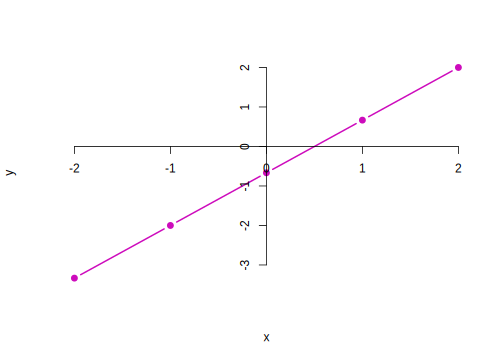
\includegraphics{fy_Alectnotes_files/figure-latex/t01-eqex-graph-1.pdf}
\caption{\label{fig:t01-eqex-graph}Graphing some solutions of \(4x-3y=2\).}
\end{figure}

The graph of the set of solutions of a linear equation in two variables is always a straight line.

\begin{center}\rule{0.5\linewidth}{0.5pt}\end{center}

\hypertarget{solving-a-pair-of-linear-equations-in-two-variables}{%
\section{Solving a pair of linear equations in two variables}\label{solving-a-pair-of-linear-equations-in-two-variables}}

\begin{example}
\protect\hypertarget{exm:unnamed-chunk-5}{}{\label{exm:unnamed-chunk-5} }\begin{align}
x+2y &= -2
\tag{A} \\
2x+3y &=1
\tag{B}
\end{align}
\end{example}

\hypertarget{by-substitution}{%
\subsection{By substitution}\label{by-substitution}}

\begin{longtable}[]{@{}
  >{\raggedright\arraybackslash}p{(\columnwidth - 4\tabcolsep) * \real{0.07}}
  >{\raggedright\arraybackslash}p{(\columnwidth - 4\tabcolsep) * \real{0.38}}
  >{\raggedright\arraybackslash}p{(\columnwidth - 4\tabcolsep) * \real{0.42}}@{}}
\toprule
\endhead
1 & Express \(x\) from (A): & \(x=-2-2y\) \\ \addlinespace
2 & Substitute into (B): & \(2(-2-2y)+3y=1\) \\ \addlinespace
3 & Multiply out: & \(-4-4y+3y=1\) \\ \addlinespace
4 & Rearrange: & \(y=-5\) \\ \addlinespace
5 & Substitute back into (A): & \(x + 2(-5)=-2\) \\ \addlinespace
6 & Rearrange: & \(x=8\) \\ \addlinespace
\bottomrule
\end{longtable}

\hypertarget{by-elimination}{%
\subsection{By elimination}\label{by-elimination}}

\begin{longtable}[]{@{}
  >{\raggedright\arraybackslash}p{(\columnwidth - 6\tabcolsep) * \real{0.06}}
  >{\raggedright\arraybackslash}p{(\columnwidth - 6\tabcolsep) * \real{0.39}}
  >{\raggedright\arraybackslash}p{(\columnwidth - 6\tabcolsep) * \real{0.35}}
  >{\raggedright\arraybackslash}p{(\columnwidth - 6\tabcolsep) * \real{0.20}}@{}}
\toprule
\endhead
1 & Multiply (A) by 2: & \(2x+4y=-4\) & Call this (A') \\ \addlinespace
2 & Subtract (A') from (B): & \(-y = 5\) & \\ \addlinespace
3 & Rearrange: & \(y=-5\) & \\ \addlinespace
4 & Substitute into (A) (as above) & \(x=8\) & \\ \addlinespace
\bottomrule
\end{longtable}

\emph{Extra Note (non-examinable)}: For ``2-by-2'' systems like these, the two methods are about the same complexity. However for larger systems of linear equations, the latter leads to a quite effective method called \emph{Gaussian elimination}, which is also amenable to be implemented as a computer algorithm.

\hypertarget{graphical-illustration}{%
\subsection{Graphical illustration}\label{graphical-illustration}}

The solutions of the equation (A) \emph{alone} lie on some straight line. Likewise for the set of solutions of the equation (B). The solutions of the system of equations, i.e.~both equations simultaneously, are exactly the point(s) where do these two lines intersect. For a sketch for the system (A),(B) above, see Figure \ref{fig:t01-system}.

\begin{figure}
\centering
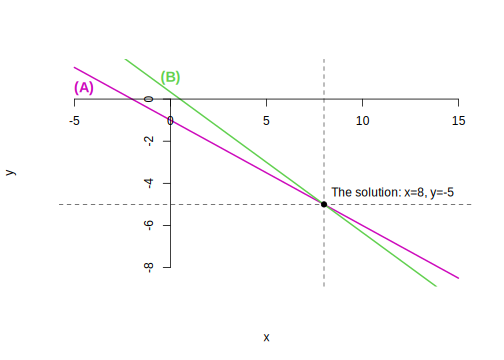
\includegraphics{fy_Alectnotes_files/figure-latex/t01-system-1.pdf}
\caption{\label{fig:t01-system}Solutions of (A) and (B) graphically}
\end{figure}

\begin{center}\rule{0.5\linewidth}{0.5pt}\end{center}

\emph{Extra Note (non-examinable)}: This is a general principle. Two lines in a plane can intersect either:

\begin{enumerate}
\def\labelenumi{\alph{enumi})}
\tightlist
\item
  at a single point, or
\item
  at a line, or
\item
  not at all.
\end{enumerate}

These are exactly the options for the set of solution of a pair of linear equations in two variables. Such a system can have:

\begin{enumerate}
\def\labelenumi{\alph{enumi})}
\tightlist
\item
  a unique solution, or
\item
  infinitely many solutions, arranged on a line, or
\item
  no solutions.
\end{enumerate}

Going to higher dimensions (more equations and more unknowns), the sets of solutions of \emph{linear} equations are always ``flats'' in a higher dimensional space (the dimension corresponds to the number of unknowns).

\hypertarget{exercises-1-simultaneous-equations}{%
\chapter*{Exercises 1 (Simultaneous Equations)}\label{exercises-1-simultaneous-equations}}
\addcontentsline{toc}{chapter}{Exercises 1 (Simultaneous Equations)}

Solve the following equations by elimination and check your results:

\begin{enumerate}
\def\labelenumi{\arabic{enumi}.}
\item
  \begin{align*}
  3x+4y &= 11\\
  x+7y  &= 15
  \end{align*}
\item
  \begin{align*}
  2x+3y &= 16\\
  3x+2y &= 14
  \end{align*}
\end{enumerate}

Solve the following equations by substitution and check your results:

\begin{enumerate}
\def\labelenumi{\arabic{enumi}.}
\setcounter{enumi}{2}
\item
  \begin{align*}
  5x+3y &= 29\\
  \frac{3x}{4}-\frac{2y}{5} &= \frac{3}{10}
  \end{align*}
\item
  \begin{align*}
  \frac{2x}{3}-\frac{y}{4} &= \frac{7}{12}\\
  4x+7y &= 37
  \end{align*}
\item
  \begin{align*}
  \frac{x}{4}+\frac{y}{5} &= \frac{3}{2}\\
  \frac{2x}{7}-\frac{y}{4} &= \frac{5}{14}
  \end{align*}
\item
  \begin{align*}
  \frac{x}{2}+\frac{y}{3} &= \frac{13}{6}\\
  2x+3y &= 19
  \end{align*}
\item
  During a lab experiment on force resolution, the following equations were found:
  \begin{align*}
  9F_H - 1.5F_V &= 7.5\\
  6.25 F_H - 2.5 F_V &= 8.75
  \end{align*}
  Determine the values of both the horizontal and the vertical force components and check your results.
\item
  A weight being moved against a frictional force is related by the law
  \[F=aW+b,\]
  where \(a\) and \(b\) are constants. When \(F=6\), \(W=7.5\), and when
  \(F=2.7\), \(W=2\). Determine the value of the constants \(a\) and \(b\) and check
  your results.
\end{enumerate}

Solve by substitution:

\begin{enumerate}
\def\labelenumi{\arabic{enumi}.}
\setcounter{enumi}{8}
\item
  \begin{align*}
  y &= 2x\\
  3x+2y &= 21
  \end{align*}
\item
  \begin{align*}
     y &= 3x-7\\
     5x-3y &= 1
     \end{align*}
\item
  \begin{align*}
     x &= 5y-3\\
     3x-8y &= 12
     \end{align*}
\item
  \begin{align*}
     2x -y &= 10\\
     3x+2y &= 29
     \end{align*}
\item
  \begin{align*}
     \frac{y}{2}-x &= 2\\
     6x-\frac{3y}{2} &= 3
     \end{align*}
\item
  \begin{align*}
     \frac{x}{2}-\frac{y}{3} &= \frac{1}{6}\\
     \frac{y}{2}-\frac{x}{6} &= 5
     \end{align*}
\item
  The cost of 4 ties and 6 pairs of socks was £68, while that of 5 ties and 8 pairs of
  socks was £87.40. What were the prices of a tie and a pair of socks, respectively?
\item
  The bill for the telephone for a quarter can be expressed in the form
  \[C = a+ \frac{nb}{100},\]
  where \(C\) is the total cost in pounds, \(a\) is the fixed charge, \(n\) is the
  number of calls, and \(b\) is the price of each call in pence. When 104 calls
  were made, the bill was £58.30, and when 67 calls were made, the bill was £50.90.
  Find the fixed charge and the cost of each call.
\end{enumerate}

\emph{Solutions:} \textbf{1.} \(x=1,y=2\); \textbf{2.} \(x=2,y=4\); \textbf{3.} \(x=2.941, y=4.765\);
\textbf{4.} \(x=2.353,y=3.941\); \textbf{5.} \(x=3.731, y=2.836\); \textbf{6.} \(x=0.2,y=6.2\);
\textbf{7.} \(F_H=0.43, F_V=-2.43\); \textbf{8.} \(a=0.6,b=1.5\);
\textbf{9.} \(x=3, y=6\); \textbf{10.} \(x=5,y=8\); \textbf{11.} \(x=12, y=3\); \textbf{12.} \(x=7,y=4\);
\textbf{13.} \(x=3,y=10\); \textbf{14.} \(x=9,y=13\); \textbf{15.} tie £9.80, socks £4.80;
\textbf{16.} fixed charge £37.50, call 20p;

\hypertarget{factorising}{%
\chapter{Factorising}\label{factorising}}

\hypertarget{multiplying-out-brackets}{%
\section{Multiplying out brackets}\label{multiplying-out-brackets}}

\begin{align*}
3\cdot(2+4) &= 3\cdot 6 = 18\\
=\quad\quad\\
3\cdot2 + 3\cdot 4 &= 6+12 = 18
\end{align*}

\begin{figure}

{\centering 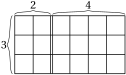
\includegraphics{t02-distrib} 

}

\caption{Illustrate distributivity with a rectangle area}\label{fig:unnamed-chunk-8}
\end{figure}

\textbf{General rules}: \(a(b+c)=ab+ac\) and \(a(b-c) = ab-ac\).

\begin{example}
\protect\hypertarget{exm:unnamed-chunk-9}{}{\label{exm:unnamed-chunk-9} }\(4(6x-2)=4\cdot 6x - 4\cdot 2 = 24x-12\).
\end{example}
\begin{example}
\protect\hypertarget{exm:unnamed-chunk-10}{}{\label{exm:unnamed-chunk-10} }\((x+2y)(y-1)=(x+2y)\cdot y - (x+2y)\cdot 1\) \(= xy+2y\cdot y - x -2y\) \(= xy-2y^2-x-2y\).
\end{example}
\begin{example}
\protect\hypertarget{exm:unnamed-chunk-11}{}{\label{exm:unnamed-chunk-11} }\((a-b+3)(4a+2)=(a-b+3)\cdot4a + (a-b+3)\cdot 2\) \(=a\cdot 4a - b\cdot 4a + 3\cdot 4a + a\cdot 2 - b\cdot 2 + 3\cdot 2\) \(= 4a^2 - 4ab + 14a - 2b+6\).
\end{example}
\begin{example}
\protect\hypertarget{exm:unnamed-chunk-12}{}{\label{exm:unnamed-chunk-12} }\((3x+1)(y-2)(x+y)=(3x+1)\cdot(y-2)\cdot x + (3x+1)\cdot(y-2)\cdot y\) \(=(3x+1)\cdot(yx-2x) + (3x+1)\cdot(y^2-2y)\) \(= (3x+1)\cdot yx - (3x+1)\cdot 2x + (3x+1)\cdot y^2 - (3x+1)\cdot 2y\) \(= 3x^2y + xy - 6x^2 - 2x + 3xy^2 + y^2 - 6xy - 2y\).
\end{example}

\hypertarget{factorising-1}{%
\section{Factorising}\label{factorising-1}}

\textbf{Factors} are the individual constituents of a \emph{product} expression.

For example: \(1\cdot 2\cdot 2\cdot 3\), ~~ \(x(y+z)\), ~~ \((a+b)(b+3)\)

\textbf{Factorising} is writing something as a product.

For example: \(12 = 1\cdot 2\cdot 2\cdot 3\).

For numbers: a whole number \(a>0\) is \textbf{a factor of a number \(b\)}, if \(\frac{b}{a}\) is also a whole number.

For example, the factors of \(24\) are \(1,2,3,6,8,12,24\).

\(24 = 2\cdot 12 = 3\cdot 8 = 4\cdot 6 = 2\cdot 2\cdot 6 = 3\cdot2\cdot 4 = 2\cdot 2\cdot 2\cdot 3 = 2^3\cdot 3\).

Factors of \(29\) are \(1\) and \(29\).

Factors of a whole number \(a\) always include \(1\) and \(a\).

A positive whole number \(p\neq1\) is called a \textbf{prime number} if it does not have factors other than \(1\) and \(p\).

First prime numbers: \(2,3,5,7,11,13,17,19,23,29,\dots\)

\begin{example}
\protect\hypertarget{exm:unnamed-chunk-13}{}{\label{exm:unnamed-chunk-13} }Factorise \(27+81\).
\end{example}
\begin{solution}
\iffalse{} {Solution. } \fi{}\(27+81 = 27(1+3)=27\cdot 4 = 3\cdot3\cdot3\cdot2\cdot2\).
\end{solution}

\begin{example}
\protect\hypertarget{exm:unnamed-chunk-15}{}{\label{exm:unnamed-chunk-15} }Factorise \(x^3-3x^2y\).
\end{example}
\begin{solution}
\iffalse{} {Solution. } \fi{}\(x^3-3x^2y = x^2(x-3y)\).
\end{solution}

\begin{example}
\protect\hypertarget{exm:unnamed-chunk-17}{}{\label{exm:unnamed-chunk-17} }Factorise \(6ax+3ay+2bx+by\).
\end{example}
\begin{solution}
\iffalse{} {Solution. } \fi{}\((6ax+3ay)+(2bx+by) = 3a(2x+y)+b(2x+y)\) \(=(3a+b)(2x+y)\).
\end{solution}

\begin{example}
\protect\hypertarget{exm:unnamed-chunk-19}{}{\label{exm:unnamed-chunk-19} }Factorise \(3x^2-5xy-2y^2\).
\end{example}
\begin{solution}
\iffalse{} {Solution. } \fi{}Note: \(-5=1\cdot 1-2\cdot 3\).
So \(3x^2-5xy-2y^2\) \(=3x^2- 6xy + xy-2y^2\) \(=3x(x-2y)+y(x-2y)\) \(=(3x+y)(x-2y)\).
\end{solution}

\begin{example}
\protect\hypertarget{exm:unnamed-chunk-21}{}{\label{exm:unnamed-chunk-21} }Factorise \(25x^2y^2-30xy+9\).
\end{example}
\begin{solution}
\iffalse{} {Solution. } \fi{}\(25x^2y^2-30xy+9\) \(=25x^2y^2 -15xy -15xy +9\) \(=5xy(5xy-3)-3(5xy-3)\) \(=(5xy-3)(5xy-3)\).
\end{solution}

\begin{example}
\protect\hypertarget{exm:unnamed-chunk-23}{}{\label{exm:unnamed-chunk-23} }Factorise \(10a^2+ab-21b^2\).
\end{example}
\begin{solution}
\iffalse{} {Solution. } \fi{}\(10a^2+ab-21b^2\) \(=10a^2 +15ab - 14ab -21b^2\) \(=(2a+3b)(5a-7b)\).
\end{solution}

\emph{Notes:}

\begin{itemize}
\tightlist
\item
  It is not always possible to sensibly factorise a given expression.
\item
  Positive whole numbers can be always factorised (uniquely in the appropriate sense) as a product of prime numbers.
\item
  Useful formula: \fbox{\(a^2-b^2=(a-b)(a+b)\)}.
\end{itemize}

\hypertarget{exercises-2-factorising}{%
\chapter*{Exercises 2 (Factorising)}\label{exercises-2-factorising}}
\addcontentsline{toc}{chapter}{Exercises 2 (Factorising)}

Multiply out of following brackets and show that:

\begin{enumerate}
\def\labelenumi{\arabic{enumi}.}
\item
  \((x+2)(x+4) = x^2 + 6x + 8\)
\item
  \((-x-7)(2-3x)=3x^2+19x-14\)
\item
  \((7t+6)(5t+8)=35t^2+86t+48\)
\item
  \((s-5)(s+6) = s^2+s-30\)
\item
  \((2q+3)(3q-5)=6q^2-q-15\)
\item
  \((x-4)(3x-1) = 3x^2-13x +4\)
\item
  \((x-2)(x+2)=x^2-4\)
\item
  \((2x-1)(2x-1) = 4x^2-4x+1\)
\item
  \((x+4)^2 = x^2 + 8x + 16\)
\item
  \((3x+5)^2=9x^2+30x+25\)
\end{enumerate}

Factorise the following quadratic polynomials:

\begin{enumerate}
\def\labelenumi{\arabic{enumi}.}
\setcounter{enumi}{10}
\item
  \(x^2+8x+15\)
\item
  \(x^2+11x+28\)
\item
  \(x^2+7x+6\)
\item
  \(x^2-10x+9\)
\item
  \(x^2-6x+9\)
\item
  \(x^2+5x-14\)
\item
  \(x^2-4x-5\)
\item
  \(x^2-10x-24\)
\item
  \(x^2-1\)
\item
  \(x^2-16\)
\item
  \(4+5x+x^2\)
\item
  \(2x^2-3x+1\)
\item
  \(9x^2-6x+1\)
\item
  \(9+6x+x^2\)
\item
  \(x^2+2ax+a^2\)
\item
  \(4x^2-9\)
\item
  \(6x^2+x-12\)
\item
  \(4x^2-11x+6\)
\item
  \(4x^2+3x-1\)
\item
  \(3x^2 - 17x+10\)
\item
  \(25x^2-16\)
\item
  \(3-2x-x^2\)
\item
  \(x^2+2xy+y^2\)
\item
  \(9-4x^2\)
\item
  \(x^2-y^2\)
\item
  \(81x^2-36xy+4y^2\)
\item
  \(49-84x+36x^2\)
\item
  \(36x^2+60xy+25y^2\)
\item
  \(4x^2-4xy-3y^2\)
\item
  \(49p^2q^2 - 28pq +4\)
\end{enumerate}

\emph{Solutions:}
\textbf{11.} \((x+3)(x+5)\)
\textbf{12.} \((x+7)(x+4)\)
\textbf{13.} \((x+6)(x+1)\)
\textbf{14.} \((x-9)(x-1)\)
\textbf{15.} \((x-3)(x-3)\)
\textbf{16.} \((x+7)(x-2)\)
\textbf{17.} \((x-5)(x+1)\)
\textbf{18.} \((x-12)(x+2)\)
\textbf{19.} \((x+1)(x-1)\)
\textbf{20.} \((x+4)(x-4)\)
\textbf{21.} \((x+1)(x+4)\)
\textbf{22.} \((2x-1)(x-1)\)
\textbf{23.} \((3x-1)(3x-1)\)
\textbf{24.} \((x+3)(x+3)\)
\textbf{25.} \((x+a)(x+a)\)
\textbf{26.} \((2x+3)(2x-3)\)
\textbf{27.} \((2x+3)(3x-4)\)
\textbf{28.} \((x-2)(4x-3)\)
\textbf{29.} \((4x-1)(x+1)\)
\textbf{30.} \((3x-2)(x-5)\)
\textbf{31.} \((5x-4)(5x+4)\)
\textbf{32.} \((3+x)(1-x)\)
\textbf{33.} \((x+y)(x+y)\)
\textbf{34.} \((3-2x)(3+2x)\)
\textbf{35.} \((x-y)(x+y)\)
\textbf{36.} \((9x-2y)(9x-2y)\)
\textbf{37.} \((7-6x)(7-6x)\)
\textbf{38.} \((6x+5y)(6x+5y)\)
\textbf{39.} \((2x-3y)(2x+y)\)
\textbf{40.} \((7pq-2)(7pq-2)\)

\hypertarget{quadratic-equations}{%
\chapter{Quadratic equations}\label{quadratic-equations}}

A \textbf{quadratic polynomial} is an expression of the form \(ax^2+bx+c\), where \(a,b,c\) are constants and \(a\neq0\).
Any value of \(x\) that makes the equation \(ax^2+bx+c=0\) hold true is called a \textbf{root} of the polynomial \(ax^2+bx+c\). The \textbf{graph} of the polynomial \(f(x)=ax^2+bx+c\) consists of all points \((x,y)\) in the plane that satisfy \(y=f(x)\).

\begin{figure}
\centering
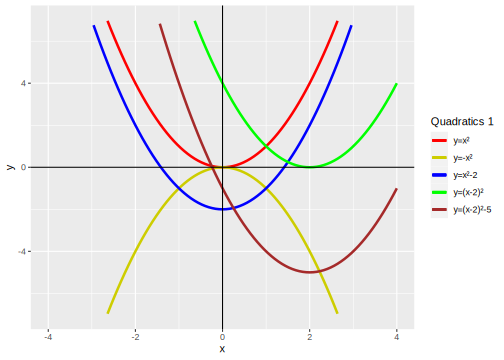
\includegraphics{fy_Alectnotes_files/figure-latex/t03-quadratic-1-1.pdf}
\caption{\label{fig:t03-quadratic-1}Examples of graphs of quadratic functions 1}
\end{figure}

\begin{figure}
\centering
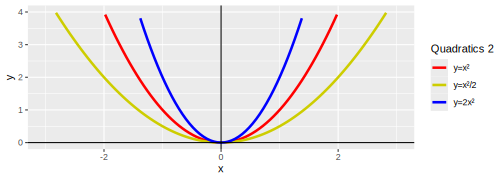
\includegraphics{fy_Alectnotes_files/figure-latex/t03-quadratic-2-1.pdf}
\caption{\label{fig:t03-quadratic-2}Examples of graphs of quadratic functions 2}
\end{figure}

\begin{example}
\protect\hypertarget{exm:unnamed-chunk-27}{}{\label{exm:unnamed-chunk-27} }Find the roots of \(2x^2-x-6\).
\end{example}
\begin{solution}
\iffalse{} {Solution. } \fi{}First factorise: \(2x^2-x-6 = (2x+3)(x-2)\).\\
Thus the roots are \(x_1=-\frac{3}{2}\) and \(x_2=2\).
\end{solution}

\begin{example}
\protect\hypertarget{exm:unnamed-chunk-29}{}{\label{exm:unnamed-chunk-29} }Find the roots of \(4x^2+4x+1\).
\end{example}
\begin{solution}
\iffalse{} {Solution. } \fi{}Factorise: \(4x^2+4x+1=(2x+1)(2x+1)=(2x+1)^2\).\\
Hence the only root is \(x_1=-\frac{1}{2}\).
\end{solution}

\begin{example}
\protect\hypertarget{exm:unnamed-chunk-31}{}{\label{exm:unnamed-chunk-31} }Find the roots of \(x^2-2x+2\).
\end{example}
\begin{solution}
\iffalse{} {Solution. } \fi{}We can rewrite \(x^2-2x+2=(x-1)^2+1\).\\
This is positive for all real numbers \(x\), thus there are no roots.
\end{solution}

\hypertarget{general-formula-for-roots-of-ax2bxc}{%
\section{\texorpdfstring{General formula for roots of \(ax^2+bx+c\)}{General formula for roots of ax\^{}2+bx+c}}\label{general-formula-for-roots-of-ax2bxc}}

\begin{enumerate}
\def\labelenumi{\arabic{enumi}.}
\tightlist
\item
  Case: \(b^2-4ac < 0\): no roots
\item
  Case: \(b^2-4ac = 0\): exactly one root \(x_1=-\frac{b}{2a}\).
\item
  Case: \(b^2-4ac > 0\): two roots \(x_{1,2}=\dfrac{-b\pm\sqrt{b^2-4ac}}{2a}\).
\end{enumerate}

Learn this by heart!

Remarks:

\begin{itemize}
\tightlist
\item
  The number \(b^2-4ac\) is sometimes referred to as the \emph{discriminant} of the quadratic.
\item
  A derivation of this formula in included at the end of the the chapter.
\end{itemize}

\begin{example}
\protect\hypertarget{exm:unnamed-chunk-33}{}{\label{exm:unnamed-chunk-33} }Find the roots of \(x^2+3x+1\).
\end{example}
\begin{solution}
\iffalse{} {Solution. } \fi{}\(x_{1,2}=\dfrac{-3\pm\sqrt{3^2-4\cdot1\cdot1}}{2\cdot 1}\) \(\dfrac{-3\pm\sqrt{9-4}}{2}\) \(=-\dfrac{3}{2}\pm\dfrac{1}{2}\sqrt{5}\).
\end{solution}

\begin{example}
\protect\hypertarget{exm:unnamed-chunk-35}{}{\label{exm:unnamed-chunk-35} }Find the roots of \(x^2-9\).
\end{example}
\begin{solution}
\iffalse{} {Solution. } \fi{}\(x_{1,2}=\dfrac{-0\pm\sqrt{0-4\cdot1\cdot(-9)}}{2\cdot1}\) \(=\pm\dfrac{36}{2}=\pm 3\).
\end{solution}

\begin{example}
\protect\hypertarget{exm:unnamed-chunk-37}{}{\label{exm:unnamed-chunk-37} }Find the roots of \(4x^2-4x+1\).
\end{example}
\begin{solution}
\iffalse{} {Solution. } \fi{}\(x_{1,2}=\dfrac{-4\pm\sqrt{(-4)^2-4\cdot 4\cdot 1}}{2\cdot 8}\) \(=\dfrac{4\pm\sqrt{0}}{8}=\dfrac{1}{2}\) (only one solution).
\end{solution}

\begin{example}
\protect\hypertarget{exm:unnamed-chunk-39}{}{\label{exm:unnamed-chunk-39} }Solve the simultaneous equations
\begin{align*}
y &= -x^2+2x+2 \tag{A}\\
x+y-2 &=0 \tag{B}
\end{align*}
\end{example}
\begin{solution}
\iffalse{} {Solution. } \fi{}Make \(x\) the subject of (B): \(x=-y+2\).\\
Substitute into (A): \(y=-(-y+2)^2+2(-y+2)+2\).\\
Rearrange: \(y^2-y-2=0\).\\
Solve the quadratic: \(y_{1,2}=\dfrac{-(-1)\pm\sqrt{(-1)^2-4\cdot1\cdot(-2)}}{2\cdot1} = \dfrac{1\pm\sqrt{9}}{2}\)\\
\(\implies\) ~ \(y_1=2\), ~~ \(y_2=-1\).\\
Substitute back into (B): ~ \(x_1=0\), ~~ \(x_2=3\).
\end{solution}

\begin{figure}
\centering
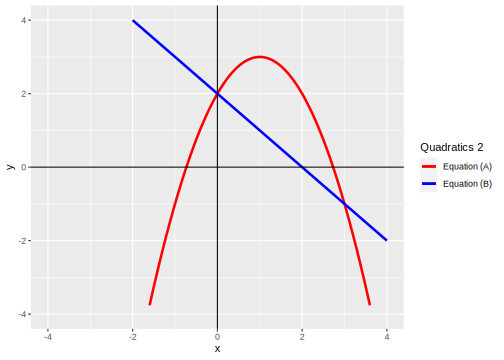
\includegraphics{fy_Alectnotes_files/figure-latex/t03-linquad-system-1.pdf}
\caption{\label{fig:t03-linquad-system}Graphical illustration of the solutions of simultaneous linear+quadratic system}
\end{figure}

\hypertarget{deriving-the-quadratic-formula}{%
\section{Deriving the quadratic formula}\label{deriving-the-quadratic-formula}}

\emph{This material is not examinable.}

\emph{Why does the quadratic formula ``work''? In other words, a ``proof''.}

The following computation shows how to derive the general formula for the roots of a quadratic polynomial.

\begin{align*}
ax^2+bx+c &= 0\\
ax^2 + bx &= -c\\
x^2 + \tfrac{b}{a}x &= -\tfrac{c}{a} \quad\text{(using $a\not=0$)}\\
x^2 + \tfrac{b}{a}x + \left(\tfrac{b}{2a}\right)^2 &= -\tfrac{c}{a} + \left(\tfrac{b}{2a}\right)^2
\end{align*}
This trick (adding \(\left(\tfrac{b}{2a}\right)^2\) to both sides) is called ``completing the square''.
\begin{align*}
\left(x+\tfrac{b}{2a}\right)^2 &= \tfrac{b^2-4ac}{(2a)^2}\\
x+\tfrac{b}{2a} &= \frac{\pm\sqrt{b^2-4ac}}{2a}\\ %\quad\text{(when $b^2-4ac\geq 0$)}
\end{align*}
The last step is only valid when \(b^2-4ac\geq 0\)!\\
One should be careful when taking square roots on both sides of an equation --- which is why there is ``\(\pm\)''.
\[
x = \frac{-b\pm\sqrt{b^2-4ac}}{2a}.
\]

\begin{center}\rule{0.5\linewidth}{0.5pt}\end{center}

\emph{Extra Note (non-examinable):} For quadratic equations, there are formulas (depending only on the numbers appearing in the equation itself) which allow us to very easily determine how many solutions does the equation have, and what are they. This situation is rather rare -- for example, if we stay with equations with a single variable \(x\) but allow the power of \(x\) to be higher, we very quickly run into issues: There is a general formula for degree \(3\), but it is rather unpleasantly complicated. From degree \(5\) onwards, it is possible to \emph{prove} that no such formula can exist in general. That is not to say that we can't solve \emph{some} high-degree equations, but there is no general formula which is guaranteed to always work. \href{https://en.wikipedia.org/wiki/Galois_theory}{This wikipedia page} goes in that direction.

Note - here we are talking about \emph{exact} solutions. In practice, problems are almost always solved numerically, obtaining \emph{approximate} solutions.

\hypertarget{exercises-3-quadratic-equations}{%
\chapter*{Exercises 3 (Quadratic equations)}\label{exercises-3-quadratic-equations}}
\addcontentsline{toc}{chapter}{Exercises 3 (Quadratic equations)}

\begin{enumerate}
\def\labelenumi{\arabic{enumi}.}
\item
  Draw the graphs of the quadratic functions given below and indicate clearly where the curves intersect the \(x\) and \(y\) axes.

  \begin{enumerate}
  \def\labelenumii{\roman{enumii})}
  \tightlist
  \item
    \(y=(x+1)^2-1\)
  \item
    \(y=-(x+1)^2-1\)
  \item
    \(y=(x+2)^2-3\)
  \item
    \(y=(x+2)^2+3\)
  \item
    \(y=-(x+2)^2+3\)
  \end{enumerate}
\item
  Solve the following quadratic equations by the method of factorisation:

  \begin{enumerate}
  \def\labelenumii{\roman{enumii})}
  \tightlist
  \item
    \(x^2-x-6=0\)
  \item
    \(x^2-16=0\)
  \item
    \(x^2-2x=0\)
  \item
    \(x^2-6x+9=0\)
  \item
    \(6x^2+18x+12=0\)
  \item
    \(6p^2-31p+35=0\)
  \item
    \(6x^2-11x-7=0\)
  \item
    \(-3r^2-14r+5=0\)
  \item
    \(14x^2=29x-12\)
  \end{enumerate}
\item
  Solve the following quadratic equations using the formula:

  \begin{enumerate}
  \def\labelenumii{\roman{enumii})}
  \tightlist
  \item
    \(3x^2-8x+2=0\)
  \item
    \(-2x^2+3x+7=0\)
  \item
    \(4x^2-3x-2=0\)
  \item
    \(7r^2+8r-2=0\)
  \item
    \(x^2+x+\frac14=\frac19\)
  \item
    \(5x^2-4x-1=0\)
  \item
    \(2a^2-5.3a+1.25=0\)
  \item
    \(x(x+4)+2x(x+3)=5\)
  \item
    \(\frac{3}{2x-3}-\frac{2}{x+1}=5\)
  \item
    \(\frac{2}{x+2}+\frac{3}{x+1}=5\)
  \end{enumerate}
\item
  Solve the following non-linear simultaneous equations:

  \begin{enumerate}
  \def\labelenumii{\roman{enumii})}
  \tightlist
  \item
    \(p-2q=1\), ~~ \(p^2-3pq+4q^2=11\)
  \item
    \(x+y=1\), ~~ \(3x^2-xy+y^2=37\)
  \item
    \(x-y=2\), ~~ \(x^3-y^3=152\)
  \item
    \(y=x^2+5x-3\), ~~ \(y=3x-2\)
  \item
    \(2a^2+ab-b^2=8\), ~~ \(3a+2b=5\)
  \end{enumerate}
\end{enumerate}

\hypertarget{problems-leading-to-quadratic-equations}{%
\subsubsection*{Problems leading to quadratic equations}\label{problems-leading-to-quadratic-equations}}
\addcontentsline{toc}{subsubsection}{Problems leading to quadratic equations}

\begin{enumerate}
\def\labelenumi{\arabic{enumi}.}
\setcounter{enumi}{4}
\item
  The angle in radians turned through by a shaft in \(t\) seconds is given by
  \[\theta=\omega t+\frac{\alpha t^2}{2}.\]
  Determine the time taken to complete five revolutions given that \(\omega=2.7\, \mathrm{rad/s}\) and \(\alpha=0.8\, \mathrm{rad/s^2}\).
\item
  In a right angled triangle the hypotenuse is twice as long as one of the sides forming the right angle. The remaining side is \(80\,\mathrm{mm}\) long. Calculate the area of the triangle.
\item
  The shape shown below has an area of \(600\,\mathrm{mm^2}\). Determine the radius \(r\).
\end{enumerate}

\begin{center}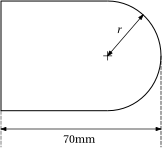
\includegraphics{t03-shape1} \end{center}

\begin{enumerate}
\def\labelenumi{\arabic{enumi}.}
\setcounter{enumi}{7}
\item
  The total surface area of a cylinder whose ends are enclosed is \(0.29\,\mathrm{m^2}\). If the height of the cylinder is \(75\,\mathrm{mm}\), determine the radius.
\item
  If the area of the shape below is \(9693\,\mathrm{mm^2}\), determine the radius \(r\).
\end{enumerate}

\begin{center}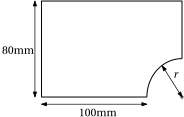
\includegraphics{t03-shape2} \end{center}

\begin{enumerate}
\def\labelenumi{\arabic{enumi}.}
\setcounter{enumi}{9}
\tightlist
\item
  A motorist travels \(84\,\mathrm{km}\) from one city to another. On the return journey, the average speed was increased by \(4\,\mathrm{km/h}\) and the journey took \(30\) minutes less. What was the average speed for the first part of the trip and how long did it take for the double journey?
\end{enumerate}

\emph{Solutions:}
\textbf{2.} (i) \(x=-2,x=3\); (ii) \(x=4,x=-4\); (iii) \(x=0,x=2\); (iv) \(x=3\) (double); (v) \(x=-1,x=-2\); (vi) \(p=7/2, p=5/3\); (vii) \(x=7/3,x=-1/2\); (viii) \(r=1/3,r=-5\); (ix) \(x=4/7,x=3/2\)

\textbf{3.} (i) \(x=2.39,x=0.28\); (ii) \(x=-1.26,x=2.76\); (iii) \(x=1.17,x=-0.42\); (iv) \(x=0.21,x=-1.35\); (v) \(x=-1/6,x=-5/6\); (vi) \(x=1,x=-1/5\); (vii) \(a=2.39,a=0.26\); (viii) \(x=0.44,x=-3.77\); (ix) \(x=1.76,x=-1.36\); (x) \(x=-0.22,x=-1.77\)

\textbf{4.} (i) \(p=-4,q=-5/2\) or \(p=5,q=2\); (ii) \(x=3,y=-2\) or \(x=-12/5,y=17/5\); (iii) \(x=6,y=4\) or \(x=-4,y=-6\); (iv) \(x=0.41,y=-0.77\) or \(x=-2.41,y=-9.23\); (v) \(a=3,b=-2\) or \(a=2.7,b=-1.55\)

\textbf{5.} \(t=6.1\,\mathrm{s}\); \textbf{6.} \(1848\,\mathrm{mm}^2\); \textbf{7.} \(r=4.36\,\mathrm{mm}\); \textbf{8.} \(r=180\,\mathrm{mm}\); \textbf{9.} \(r=71.86\,\mathrm{mm}\) or \(r=30\,\mathrm{mm}\); \textbf{10.} \(6.5\) hours

\hypertarget{inequalities}{%
\chapter{Inequalities}\label{inequalities}}

For two numbers \(a\) and \(b\):

\begin{itemize}
\tightlist
\item
  \(a<b\) means that \(a\) is less than \(b\)
\item
  \(a>b\) means that \(a\) is greater than \(b\)
\item
  \(a\leq b\) means that \(a\) is less than or equal to \(b\)
\item
  \(a\geq b\) means that \(a\) is greater than or equal to \(b\)
\end{itemize}

For example: \(1<2\),~ \(-10<-5\),~ \(-3\leq -3\),~ \(-2\geq -4\).

Note: \(a>0\) means the same as ``\(a\) is positive''.

If \(x\) is given on the number line as

\begin{center}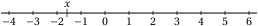
\includegraphics{t04-numline1} \end{center}

then the following hold: \(-2<x\),~ \(-1>x\),~ \(x<0\),~ \(-5<x\),~ \(x<3\).

The notation ``\(\{x : x>3\}\)'' means ``the set of all numbers \(x\) that are greater than \(3\)''.

\begin{center}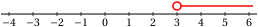
\includegraphics{t04-numline2} \end{center}

Similarly, \(\{x: x\leq -1\}\) is the set of numbers that can be represented on the number line as

\begin{center}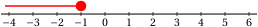
\includegraphics{t04-numline3} \end{center}

The notation \(\{x: -2\leq x <1\}\) can be depicted as

\begin{center}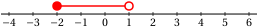
\includegraphics{t04-numline4} \end{center}

The notation \(\{x: x<-1 \text{ or } x\geq2\}\) can be depicted as

\begin{center}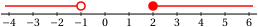
\includegraphics{t04-numline5} \end{center}

\hypertarget{axioms-of-inequalities}{%
\subsubsection*{Axioms of inequalities}\label{axioms-of-inequalities}}
\addcontentsline{toc}{subsubsection}{Axioms of inequalities}

\begin{enumerate}
\def\labelenumi{\arabic{enumi}.}
\tightlist
\item
  If \(a<b\) then \(a+c<b+c\).
\item
  If \(a<b\) then \(a-c<b-c\).
\item
  If \(a<b\) and \(c>0\), then \(ac<bc\).
\item
  If \(a<b\) and \(c<0\), then \(ac>bc\).
\end{enumerate}

For example: \(2<3\) \(\iff\) \(-2>-3\).

\begin{example}
\protect\hypertarget{exm:unnamed-chunk-50}{}{\label{exm:unnamed-chunk-50} }Solve \(3x+5>17\).
\end{example}
\begin{solution}
\iffalse{} {Solution. } \fi{}\(3x+5>17\)\\
\(\iff\) \(3x>12\) \hfill~{(subtract \(5\))}\\
\(\iff\) \(x>4\) \hfill~{(multiply by \(1/3\))}
\end{solution}

\begin{example}
\protect\hypertarget{exm:unnamed-chunk-52}{}{\label{exm:unnamed-chunk-52} }Determine the set \(\{x: 2x-x^2<3x-12\}\).
\end{example}
\begin{solution}
\iffalse{} {Solution. } \fi{}\(2x-x^2<3x-12\)\\
\(\iff\) \(2x-x^2-3x+12<0\) \hfill~{(subtract \(3x-12\))}\\
\(\iff\) \(-x^2-x+12<0\) \hfill~{(rearrange LHS)}\\
\(\iff\) \(x^2+x-12>0\) \hfill~{(multiply by \(-1\))}\\
\(\iff\) \((x+4)(x-3)>0\) \hfill~{(factorise LHS)}\\
\(\iff\) \(\big( x+4>0\) and \(x-3>0\big)\) or \(\big(x+4<0\) and \(x-3<0\big)\)\\
\(\iff\) \(\big( x>-4\) and \(x>3\big)\) or \(\big(x<-4\) and \(x<3\big)\)\\
\(\iff\) \(x>3\) or \(x<-4\)\\
Answer: \(\{x: x>3\text{ or }x<-4\}\).
\end{solution}

\begin{example}
\protect\hypertarget{exm:unnamed-chunk-54}{}{\label{exm:unnamed-chunk-54} }Solve \(\dfrac{x-1}{x-2}<0\).
\end{example}
\begin{solution}
\iffalse{} {Solution. } \fi{}\(\frac{x-1}{x-2}<0\)\\
\(\iff\) \((x-1)(x-2)<0\) \hfill~{(multiply by \((x-1)^2\geq 0\))}\\
\(\iff\) \(\big( x<1\) and \(x>2\big)\) or \(\big(x>1\) and \(x<2\big)\)\\
\(\iff\) \(1<x<2\)
\end{solution}

\begin{example}
\protect\hypertarget{exm:unnamed-chunk-56}{}{\label{exm:unnamed-chunk-56} }Solve \(\dfrac{3x-2}{1+x}\leq 1\).
\end{example}
\begin{solution}
\iffalse{} {Solution. } \fi{}\(\frac{3x-2}{1+x}\leq1\)\\
\(\iff\) \(\frac{(3x-2)-(1+x)}{1+x}\leq0\)\\
\(\iff\) \(\frac{2x-3}{1+x}\leq0\)\\
\(\iff\) \(\big( x\leq\frac{3}{2}\) and \(x>-1\big)\) or \(\big(x\geq \frac{3}{2}\) and \(x<-1\big)\)\\
\(\iff\) \(-1<x\leq\frac{3}{2}\)
\end{solution}

\hypertarget{exercises-4-inequalities}{%
\chapter*{Exercises 4 (Inequalities)}\label{exercises-4-inequalities}}
\addcontentsline{toc}{chapter}{Exercises 4 (Inequalities)}

Solve the following and illustrate the solution on the number line:

\begin{enumerate}
\def\labelenumi{\arabic{enumi}.}
\item
  \(2x+7>23\)
\item
  \(\{x: 6x-4>x\}\)
\item
  \(\{x: 2-3x \leq 2x+3\}\)
\item
  \(4x^2-9<0\)
\item
  \(x^2+3x+2\leq 5(x+2)\)
\item
  \(6x+5\geq x-5\)
\item
  \(|4x-5|<1\)
\item
  \(|-x+3|>2\)
\item
  \((3x-2)\div(1+x)<1\)
\item
  \((x+3)(x-4)<0\)
\end{enumerate}

\emph{Solutions:}
\textbf{1.} \(x>8\);
\textbf{2.} \(x>4/5\);
\textbf{3.} \(x\geq-1/5\);
\textbf{4.} \(-3/2< x< 3/2\);
\textbf{5.} \(-2\leq x\leq4\);
\textbf{6.} \(x\geq-2\);
\textbf{7.} \(1<x<3/2\);
\textbf{8.} \(x<1\) or \(x>5\);
\textbf{9.} \(-1<x<3/2\);
\textbf{10.} \(-3<x<4\)

\hypertarget{indices}{%
\chapter{Indices}\label{indices}}

\hypertarget{exponents}{%
\section{Exponents}\label{exponents}}

Subscripts and superscripts are also called \textbf{indices} (singular \textbf{index}). Subscripts are usually used to denote families of variables, for example \(a_1,a_2,a_3,\dots\) (instead of \(a,b,c\)).

A superscript usually denotes an \textbf{exponent}, i.e.~it represents the power to which a given number is raised.

\textbf{Examples:}

\begin{itemize}
\tightlist
\item
  \(4^3=\underbrace{4\cdot4\cdot4}_{3\text{ times}}=64\)
\item
  \(2^5=\underbrace{2\cdot2\cdot2\cdot2\cdot2}_{5\text{ times}}=32\)
\item
  \(x^4=\underbrace{x\cdot x\cdot x\cdot x}_{4\text{ times}}\)
\end{itemize}

In general, we \textbf{define}:

\begin{itemize}
\tightlist
\item
  \(x^n := \underbrace{x\cdot x\cdots x}_{n\text{ times}}\), when \(n>0\),
\item
  \(x^0 := 1\),
\item
  \(x^{-n} := \dfrac{1}{\underbrace{x\cdot x\cdots x}_{n\text{ times}}}\), when \(n>0\).
\end{itemize}

\textbf{Further examples:}

\begin{itemize}
\tightlist
\item
  \(x^{\frac{1}{2}} := \sqrt{x}\)~~ for \(x\geq 0\),
\item
  \(x^{\frac{1}{3}} := \sqrt[3]{x}\).
\end{itemize}

In general, we \textbf{define}:

\begin{itemize}
\tightlist
\item
  \(x^{\frac{1}{n}} := \sqrt[n]{x}\) ~~ for \(x\geq0\) and \(n>0\),
\item
  \(x^{\frac{m}{n}} := \sqrt[n]{x^m}\) ~~ for \(x\geq0\) and \(m,n>0\),
\item
  \(x^{-\frac{m}{n}} := \dfrac{1}{\sqrt[n]{x^m}}\) ~~ for \(x\geq0\) and \(m,n>0\).
\end{itemize}

\hypertarget{laws-of-exponents}{%
\section{Laws of exponents}\label{laws-of-exponents}}

The basic ones are:

\begin{enumerate}
\def\labelenumi{\arabic{enumi}.}
\item
  \fbox{\(a^r\cdot a^s = a^{r+s}\)}
\item
  \fbox{\((a\cdot b)^r = a^{r}\cdot b^{r}\)}
\item
  \fbox{\(\left(a^r\right)^s = a^{r\cdot s}\)}
\end{enumerate}

From these, one can derive the following two:

\begin{enumerate}
\def\labelenumi{\arabic{enumi}.}
\setcounter{enumi}{3}
\item
  \fbox{\(\frac{a^r}{a^s} = a^{r-s}\)}
\item
  \fbox{\(\left(\sqrt[n]{a}\right)^m = a^{\frac{m}{n}}\)}
\end{enumerate}

Deriving 4: \(\frac{a^r}{a^s} = a^r\cdot \frac{1}{a^s} = a^r\cdot a^{-s} \stackrel{1.}{=} a^{r-s}\).

Deriving 5: \(\left(\sqrt[n]{a}\right)^m = \left(a^{\frac{1}{n}}\right)^m \stackrel{3.}{=} a^{\frac{1}{n}\cdot m} = a^\frac{m}{n}\).

\begin{example}
\protect\hypertarget{exm:unnamed-chunk-60}{}{\label{exm:unnamed-chunk-60} }Write the following expressions using only positive indices: \(x^{-4}\),~ \(3x^{-4}\),~ \((3x)^{-4}\) ~ and \(\frac{2}{y^{-3}}\).
\end{example}
\begin{solution}
\iffalse{} {Solution. } \fi{}
\end{solution}
- \(x^{-4}=\frac{1}{x^4}\)
- \(3x^{-4}=3\cdot\frac{1}{x^4}=\frac{3}{x^4}\)
- \((3x)^{-4} = \frac{1}{(3x)^4} = \frac{1}{3^4\cdot x^4}=\frac{1}{81x^4}\)
- \(\frac{2}{y^{-3}}=\frac{2}{\frac{1}{y^3}}=2y^3\)

\begin{example}
\protect\hypertarget{exm:unnamed-chunk-62}{}{\label{exm:unnamed-chunk-62} }Write the following expressions using only single index: \(\left(x^2\right)^{-3}\), ~ \(\left((-x)^{-2}\right)^{-3}\), ~ \(\left(\frac{t}{t^{-2}}\right)^{4}\).
\end{example}
\begin{solution}
\iffalse{} {Solution. } \fi{}
\end{solution}
- \(\left(x^2\right)^{-3} = x^{2\cdot(-3)}=x^{-6}\)
- \(\left((-x)^{-2}\right)^{-3} = (-x)^{(-2)\cdot(-3)}=(-x)^{6}=\left((-1)\cdot x\right)^6=(-1)^6\cdot x^6=x^6\)
- \(\left(\frac{t}{t^{-2}}\right)^{4}=\frac{t^4}{(t^{-2})^4}=\frac{t^4}{t^{-8}}=t^{4-(-8)}=t^{12}\)

\begin{example}
\protect\hypertarget{exm:unnamed-chunk-64}{}{\label{exm:unnamed-chunk-64} }Simplify the expression \(A=\dfrac{x^{-6}y^{3/2}w^2}{x^{-3}w^3}\div\dfrac{x^\frac12\sqrt[3]{y}}{(xy)^3(\sqrt[4]{w})^{-2}}\) so that it uses only positive indices.
\end{example}
\begin{solution}
\iffalse{} {Solution. } \fi{}
\end{solution}
\begin{align*}
A&= \frac{x^{-6}y^{\frac{3}{2}}w^2\,(xy)^3(\sqrt[4]{w})^{-2}}{x^{-3}w^3\, x^{\frac{1}{2}}\sqrt[3]{y}}\\
&=\frac{x^{-6}y^{\frac{3}{2}}w^2x^3y^3w^{-\frac12}}{x^{-3}w^3x^{\frac12}y^{\frac13}}\\
&=x^{-6+3-(-3)-\frac12}\,y^{\frac32+3-\frac13}\, w^{2-\frac12-3}\\
&=x^{-\frac12}\,y^{\frac{25}{6}}\,w^{-\frac32}\\
&=\frac{y^{\frac{25}{6}}}{x^{\frac12}\,w^{\frac32}}.
\end{align*}

\hypertarget{scientific-notation-of-numbers}{%
\section{Scientific notation of numbers}\label{scientific-notation-of-numbers}}

\textbf{Standard} (or \textbf{normalised}) scientific notation of number is:

\begin{quote}
\(a\cdot 10^n\), ~ ~ where \(1\leq|a|<10\) and \(n\) is an integer
\end{quote}

\textbf{Engineering} scientific notation is:

\begin{quote}
\(a\cdot 1000^n\), ~ ~ where \(1\leq|a|<1000\) and \(n\) is a multiple of \(3\)
\end{quote}

The ``\(a\)'' is called \textbf{mantissa}, the ``\(n\)'' is called \textbf{exponent}.

\begin{longtable}[]{@{}
  >{\centering\arraybackslash}p{(\columnwidth - 4\tabcolsep) * \real{0.28}}
  >{\centering\arraybackslash}p{(\columnwidth - 4\tabcolsep) * \real{0.33}}
  >{\centering\arraybackslash}p{(\columnwidth - 4\tabcolsep) * \real{0.33}}@{}}
\toprule
Decimal expansion & Standard notation & Engineering notation \\ \addlinespace
\midrule
\endhead
\(17\) & \(1.7\cdot 10^1\) & \(17\) \\ \addlinespace
\(620\) & \(6.2\cdot 10^2\) & \(620\) \\ \addlinespace
\(342567\) & \(3.42567\cdot 10^5\) & \(342.567\cdot 10^3\) \\ \addlinespace
\(0.0001\) & \(1\cdot 10^{-4}\) & \(100\cdot 10^{-6}\) \\ \addlinespace
\(0.00005\) & \(5\cdot 10^{-5}\) & \(50\cdot 10^{-6}\) \\ \addlinespace
\bottomrule
\end{longtable}

\hypertarget{exercises-5-indices}{%
\chapter*{Exercises 5 (Indices)}\label{exercises-5-indices}}
\addcontentsline{toc}{chapter}{Exercises 5 (Indices)}

\begin{enumerate}
\def\labelenumi{\arabic{enumi}.}
\item
  Using the rules of indices put the following expressions in their simplest form:

  \begin{enumerate}
  \def\labelenumii{\roman{enumii})}
  \tightlist
  \item
    \(\dfrac{9^2\times 9\times 9^5}{3^9\times 3}\)
  \item
    \(\dfrac{7^6\times 7^3\times 4^8}{7^8\times 4^2\times 4^3}\)
  \end{enumerate}
\item
  Simplify the following expressions without using a calculator:

  \begin{enumerate}
  \def\labelenumii{\roman{enumii})}
  \tightlist
  \item
    \(\dfrac{(7.5\times 10^2)(1.2\times 10^3)}{4}\)
  \item
    \(\dfrac{(4.5\times 10^{-7})(1.2\times 10^9)}{9}\)
  \item
    \(\dfrac{(3.3\times10^{-5})(4.2\times 10^6)}{(1.1\times10^{-2})(2.1\times 10^3)}\)
  \item
    \(\dfrac{4^{\frac12}\times 64^{\frac23}\times 32^{\frac15}}{16^{\frac32}\times 81^{-\frac34}}\)
  \end{enumerate}
\item
  Simplify the following:

  \begin{enumerate}
  \def\labelenumii{\roman{enumii})}
  \tightlist
  \item
    \((a^2 x^3 y^{-2})^3 \times (a^{-3}xy^3)^{1/2}\div (axy^{-3})^{5/2}\)
  \item
    \(\dfrac{\sqrt[3]{a}b^{-\frac12}}{\sqrt{a^5}\sqrt{b}}\div\dfrac{ab^2c^{-\frac32}}{\sqrt{a^2b^3}c^{\frac52}}\)
  \end{enumerate}
\item
  The \emph{e.m.f.} induced in a circuit when \(N\) lines of induction are cut in a time \(t\) seconds is given by:
  \[e.m.f. = \frac{N}{t\times 10^8}.\]
  Determine the \emph{e.m.f.} induced when \(N=36\times 10^8\) and \(t=30\,\mathrm{ms}\).
\item
  Without using a calculator, determine the value of \(\left(\dfrac{81^{\frac14}\times 9^{\frac12}}{3^2\times 27^2}\right)^{-1}\).
\item
  Simplify:

  \begin{enumerate}
  \def\labelenumii{\alph{enumii})}
  \tightlist
  \item
    \(5^7\times 5^{13}\)
  \item
    \(9^8\times 9^5\)
  \item
    \(11^2\times11^3\times11^4\)
  \item
    \(\dfrac{15^3}{15^2}\)
  \item
    \(\dfrac{4^{18}}{4^9}\)
  \item
    \(\dfrac{5^{20}}{5^{19}}\)
  \item
    \(a^7a^3\)
  \item
    \(a^4a^5\)
  \item
    \(b^{11}b^{10}b\)
  \item
    \(x^{7}\times x^{8}\)
  \item
    \(y^4\times y^8\times y^9\)
  \end{enumerate}
\item
  Simplify:

  \begin{enumerate}
  \def\labelenumii{\alph{enumii})}
  \tightlist
  \item
    \((7^3)^2\)
  \item
    \((4^2)^8\)
  \item
    \((7^9)^2\)
  \item
    \(\dfrac{1}{(5^3)^8}\)
  \item
    \((x^2y^3)(x^3y^2)\)
  \item
    \((a^2bc^2)(b^2ca)\)
  \end{enumerate}
\item
  Remove the brackets from:

  \begin{enumerate}
  \def\labelenumii{\alph{enumii})}
  \tightlist
  \item
    \((x^2y^4)^5\)
  \item
    \((9x^3)^2\)
  \item
    \((-3x)^3\)
  \item
    \((-x^2y^3)^4\)
  \end{enumerate}
\item
  Simplify:

  \begin{enumerate}
  \def\labelenumii{\alph{enumii})}
  \tightlist
  \item
    \(\dfrac{(z^2)^3}{z^3}\)
  \item
    \(\dfrac{(y^3)^2}{(y^2)^2}\)
  \item
    \(\dfrac{(x^3)^2}{(x^2)^3}\)
  \end{enumerate}
\item
  Write each of the following using only a positive power:

  \begin{enumerate}
  \def\labelenumii{\alph{enumii})}
  \tightlist
  \item
    \(x^{-4}\)
  \item
    \(\dfrac{1}{x^{-5}}\)
  \item
    \(x^{-7}\)
  \item
    \(y^{-2}\)
  \item
    \(\dfrac{1}{y^{-1}}\)
  \end{enumerate}
\item
  Simplify the following and write your results using only positive powers:

  \begin{enumerate}
  \def\labelenumii{\alph{enumii})}
  \tightlist
  \item
    \(x^{-1}x^{-2}\)
  \item
    \(x^{-3}x^{-2}\)
  \item
    \(x^3x^{-4}\)
  \item
    \(x^{-4}x^9\)
  \item
    \(\dfrac{x^{-2}}{x^{11}}\)
  \item
    \((x^{-4})^2\)
  \item
    \((x^{-3})^3\)
  \item
    \((x^2)^{-2}\)
  \end{enumerate}
\item
  Simplify:

  \begin{enumerate}
  \def\labelenumii{\alph{enumii})}
  \tightlist
  \item
    \(a^{13}a^{-2}\)
  \item
    \(x^{-9}x^{-7}\)
  \item
    \(x^{-21}x^2x\)
  \end{enumerate}
\item
  Evaluate:

  \begin{enumerate}
  \def\labelenumii{\alph{enumii})}
  \tightlist
  \item
    \(10^{-3}\)
  \item
    \(10^{-4}\)
  \item
    \(10^{-5}\)
  \item
    \(\dfrac{4^{-8}}{4^{-6}}\)
  \item
    \(\dfrac{3^{-5}}{3^{-8}}\)
  \end{enumerate}
\item
  Simplify, then evaluate:

  \begin{enumerate}
  \def\labelenumii{\alph{enumii})}
  \tightlist
  \item
    \(64^{\frac13}\)
  \item
    \(144^{\frac12}\)
  \item
    \(16^{-\frac14}\)
  \item
    \(25^{-\frac12}\)
  \item
    \(\left(3^{-\frac12}\right)^4\)
  \item
    \(\left(8^{\frac13}\right)^{-1}\)
  \end{enumerate}
\end{enumerate}

\emph{Solutions:}
\textbf{1.} (i) \(3^6\); (ii) \(7\times 4^3\);
\textbf{2.} (i) \(2.25\times 10^5\); (ii) \(60\); (iii) \(6\); (iv) \(27\);
\textbf{3.} (i) \(a^2x^7y^3\); (ii) \(\frac{c^4}{a^{13/6}b^{3/2}}\);
\textbf{4.} \(1.2\times 10^3\);
\textbf{5.} \(729\);
\textbf{6.} (a) \(5^{20}\); (b) \(9^{13}\); (c) \(11^9\); (d) \(15\); (e) \(4^9\); (f) \(5\); (g) \(a^{10}\); (h) \(a^9\); (i) \(b^{22}\); (j) \(x^{15}\); (k) \(y^{21}\)
\textbf{7.} (a) \(7^6\); (b) \(4^{16}\); (c) \(7^{18}\); (d) \(5^{-24}\); (e) \(x^5y^5\); (f) \(a^3b^3c^3=(abc)^3\);
\textbf{8.} (a) \(x^{10}y^{20}\); (b) \(81x^6\); (c) \(-27x^3\); (d) \(x^8y^{12}\);
\textbf{9.} (a) \(z^3\); (b) \(y^2\); (c) \(1\);
\textbf{10.} (a) \(\frac{1}{x^4}\); (b) \(x^5\); (c) \(\frac{1}{x^7}\); (d) \(\frac{1}{y^2}\); (e) \(y\);
\textbf{11.} (a) \(\frac{1}{x^3}\); (b) \(\frac{1}{x^5}\); (c) \(\frac{1}{x}\); (d) \(x^5\); (e) \(\frac{1}{x^{13}}\); (f) \(\frac{1}{x^8}\); (g) \(\frac{1}{x^9}\); (h) \(\frac{1}{x^4}\);
\textbf{12.} (a) \(a^{11}\); (b) \(\frac{1}{x^{16}}\); (c) \(\frac{1}{x^{18}}\);
\textbf{13.} (a) \(0.001\); (b) \(0.0001\); (c) \(0.00001\); (d) \(1/16\); (e) \(27\);
\textbf{14.} (a) \(4\); (b) \(12\); (c) \(1/2\); (d) \(1/5\); (e) \(1/9\); (f) \(1/2\)

\hypertarget{logarithms}{%
\chapter{Logarithms}\label{logarithms}}

If \(a=b^x\), then \(x\) is called the \textbf{logarithm of \(a\) to the base \(b\)}. In symbols \(x=\log_b a\).

For example, \(\log_3 9=2\), ~ ~ \(\log_2 32=5\), ~ ~ \(\log_{10} 1000=3\).

We \emph{require} the base \(b\) to be a positive number, not equal to \(1\).

Notation for two most commonly used bases:

\begin{itemize}
\tightlist
\item
  \(\log(a) := \log_{10}(a)\) ~ ~ (used in Engineering)
\item
  \(\ln(a) := \log_e(a)\) ~ ~ where \(e\) is the \href{https://en.wikipedia.org/wiki/E_(mathematical_constant)}{Euler's number}, \(e \approx 2.7183\) (to 4 d.p.)
\item
  \(\ln(a)\) is also called the \textbf{natural logarithm} of \(a\).
\end{itemize}

\textbf{Note:}: \(\log_{10}(a) \begin{cases} =0 & \text{for }a=1\\ >0& \text{for }a>1\\ <0 &\text{for }0<a<1\\\text{does not exist}&\text{for }a\leq0.\end{cases}\)

\begin{figure}
\centering
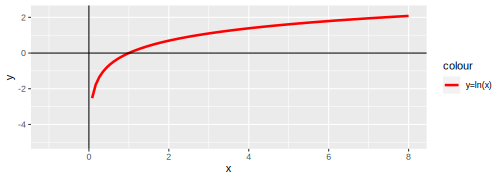
\includegraphics{fy_Alectnotes_files/figure-latex/t06-log-graph-1.pdf}
\caption{\label{fig:t06-log-graph}Graph of the natural logarithm function}
\end{figure}

\hypertarget{laws-of-logarithms}{%
\section{Laws of logarithms}\label{laws-of-logarithms}}

\begin{enumerate}
\def\labelenumi{\arabic{enumi}.}
\item
  \fbox{\(\log_b(M\cdot N)=\log_b(M)+\log_b(N)\)}
\item
  \fbox{\(\log_b(N^a)=a\cdot\log_b(N)\)}
\end{enumerate}

\emph{Proof (non-examinable):}

\begin{enumerate}
\def\labelenumi{\arabic{enumi}.}
\item
  \(\log_b(M\cdot N)\) is defined by the equation \(b^{\log_b(M\cdot N)}=M\cdot N\).\\
  So, we only need to verify that \(b^{\log_b(M)+\log_b(N)}=M\cdot N\).\\
  But by laws of exponents and the definition of logarithm, we have LHS \(= b^{\log_b(M)}\cdot b^{\log_b(N)}=M\cdot N\), so we are done.
\item
  \(\log_b(N^a)\) is defined by the equation \(b^{\log_b(N^a)}=N^a\).\\
  So, we only need to verify that \(b^{a\cdot \log_b(N)}=N^a\).\\
  But by laws of exponents and the definition of logarithm, we have LHS \(= \left(b^{\log_b(N)}\right)^a= N^a\), so we are done.
\end{enumerate}

From 1. and 2. we can derive two more laws:

\begin{enumerate}
\def\labelenumi{\arabic{enumi}.}
\setcounter{enumi}{2}
\item
  \fbox{\(\log_b\left(\frac{M}{N}\right) = \log_b(M)-\log_b(N)\)}
\item
  \fbox{\(\log_b(N) = \dfrac{\log_{10}(N)}{\log_{10}(b)}\)} \(=\dfrac{\ln(N)}{\ln(b)} = \dfrac{\log_c(N)}{\log_c(b)}\) for any base \(c\).
\end{enumerate}

\emph{Proof (non-examinable):}

\begin{enumerate}
\def\labelenumi{\arabic{enumi}.}
\setcounter{enumi}{2}
\item
  LHS \(= \log_b(M\cdot N^{-1}) \stackrel{1.}{=} \log_b(M) + \log_b(N^{-1}) \stackrel{2.}{=} \log_b(M)-\log_b(N) =\) RHS
\item
  We apply \(\log_c\) to both sides of the equation \(b^{\log_b(N)}=N\):
  \begin{align*}
   \log_c\left(b^{\log_b(N)}\right) &= \log_c(N) & \\
   \log_b(N)\cdot \log_c(b) &= \log_c(N) & \text{(by 2.)}\\
   \log_b(N) &= \frac{\log_c(N)}{\log_c(b)} & (\text{dividing by }\log_c(b)\not=0)
  \end{align*}
\end{enumerate}

\begin{example}
\protect\hypertarget{exm:unnamed-chunk-68}{}{\label{exm:unnamed-chunk-68} }\(\log_5(2.623) \stackrel{4.}{=} \dfrac{\log_{10}(2.623)}{\log_{10}(5)} \approx \dfrac{0.4188}{0.6990} \approx 0.5991\)
\end{example}

\begin{example}
\protect\hypertarget{exm:unnamed-chunk-69}{}{\label{exm:unnamed-chunk-69} }Solve \(2^x =5\).
\end{example}
\begin{solution}
\iffalse{} {Solution. } \fi{}\(x=\log_2(5)=\dfrac{\log_{10}(5)}{\log_{10}(2)} \approx\dfrac{0.6990}{0.3010}\approx 2.322\)
\end{solution}

\begin{example}
\protect\hypertarget{exm:unnamed-chunk-71}{}{\label{exm:unnamed-chunk-71} }Solve \(3^{x+1}=2^{2x-3}\).
\end{example}
\begin{solution}
\iffalse{} {Solution. } \fi{}Applying \(\log_{10}\) on both sides: \(\log_{10}(3^{x+1}) = \log_{10}(2^{2x-3})\).\\
\(\implies\) \((x+1)\log_{10}(3) = (2x-3)\log_{10}(2)\)\\
\(\implies\) \(x\left(\log_{10}(3)-2\log_{10}(2)\right) = -3\log_{10}(2)-\log_{10}(3)\)\\
\(\implies\) \(x=\dfrac{-3\log_{10}(2)-\log_{10}(3)}{\log_{10}(3)-2\log_{10}(2)}\approx 11.0471\)
\end{solution}

\begin{example}
\protect\hypertarget{exm:unnamed-chunk-73}{}{\label{exm:unnamed-chunk-73} }Solve \(2^{2x}-2^{x+1}-15=0\).
\end{example}
\begin{solution}
\iffalse{} {Solution. } \fi{}\(2^{2x}-2^{x+1}-15=0\)\\
\(\iff\) \(\left(2^x\right)^2-2\cdot\left(2^x\right)-15=0\) \hfill~{(by laws of exponents)}\\
\(\iff\) \(y^2 -2y-15=0\) \hfill~{(where \(y=2^x\))}\\
\(\iff\) \((y-5)(y+3)=0\) \hfill~{(factorising)}\\
\(\iff\) \(y=5\) or \(y=-3\)\\
\(\iff\) \(x=\log_2(5)\approx 2.322\),\\
and \(2^x=-3\) is not possible (so no solution)
\end{solution}

\hypertarget{exercises-6-logarithms}{%
\chapter*{Exercises 6 (Logarithms)}\label{exercises-6-logarithms}}
\addcontentsline{toc}{chapter}{Exercises 6 (Logarithms)}

\begin{enumerate}
\def\labelenumi{\arabic{enumi}.}
\item
  Determine the values for the following logarithms:

  \begin{enumerate}
  \def\labelenumii{\roman{enumii})}
  \tightlist
  \item
    \(\log_2 98.5\)
  \item
    \(\log_4 22.86\)
  \item
    \(\log_7 1050\)
  \item
    \(\log_8 211.746\)
  \end{enumerate}
\item
  The formula \(\dfrac{T_1}{T_2}=e^{\mu\theta}\) shows the relationship between the tension in a flat driving belt (\(T_1\) being on the tight or driving side) whilst \(\theta\) is the angle of contact around the pulley and \(\mu\) is the coefficient of friction.

  \begin{enumerate}
  \def\labelenumii{\roman{enumii})}
  \tightlist
  \item
    Show that \(\log T_1 = \log T_2 + \mu\theta\log e\)
  \item
    Determine \(T_1\) using logs if \(T_2=150\), \(\mu=0.25\), \(\theta=3\) and \(e=2.718\).
  \end{enumerate}
\item
  Solve for \(x\):

  \begin{enumerate}
  \def\labelenumii{\roman{enumii})}
  \tightlist
  \item
    \(5^{2x}=0.5\)
  \item
    \(3^{2x}+3^x=12\)
  \item
    \(3^{2x}-3^{x+1}+2=0\)
  \end{enumerate}
\item
  If \(10^x+10^{-x}=4\), show that \(x=\log_{10}(2\pm\sqrt{3})\).
\item
  Express in terms of \(\log p\), \(\log q\) and \(\log r\):

  \begin{enumerate}
  \def\labelenumii{\alph{enumii})}
  \tightlist
  \item
    \(\log pq\)
  \item
    \(\log pqr\)
  \item
    \(\log pq/r\)
  \item
    \(\log p/qr\)
  \item
    \(\log p^2q\)
  \item
    \(\log q/r^2\)
  \item
    \(\log p^2q^3/r\)
  \item
    \(\log p^nq^m\)
  \item
    \(\log 2pq\)
  \item
    \(\log 2pq^2\)
  \end{enumerate}
\item
  Simplify:

  \begin{enumerate}
  \def\labelenumii{\alph{enumii})}
  \tightlist
  \item
    \(\log p+\log q\)
  \item
    \(2\log p+\log q\)
  \item
    \(\log q-\log r\)
  \item
    \(3\log q+4\log p\)
  \item
    \(\log p+2\log q-3\log r\)
  \item
    \(\log p-\log 2\)
  \item
    \(2\log p-p\log 2\)
  \item
    \(\log(p+2)-\log(q-2)\)
  \end{enumerate}
\end{enumerate}

\emph{Solutions:}
\textbf{1.} (i) \(6.62\); (ii) \(2.26\); (iii) \(3.57\); (iv) \(2.58\);
\textbf{2.} (ii) \(T_1=317\);
\textbf{3.} (i) \(x=-0.22\); (ii) \(x=1\); (iii) \(x=0.63\) or \(x=0\);
\textbf{5.} (a) \(\log p+\log q\); (b) \(\log p+\log q+\log r\); (c) \(\log p+\log q-\log r\); (d) \(\log p-\log q-\log r\); (e) \(2\log p+\log q\); (f) \(\log q-2\log r\); (g) \(2\log p+3\log q-\log r\); (h) \(n\log p+m\log q\); (i) \(\log 2+\log p+\log q\); (j) \(\log 2+\log p+2\log q\);
\textbf{6.} (a) \(\log pq\); (b) \(\log p^2q\); (c) \(\log q/r\); (d) \(\log q^3p^4\); (e) \(\log pq^2/r^3\); (f) \(\log p/2\); (g) \(\log p^2/2^p\); (h) \(\log (p+2)/(q-2)\)

\hypertarget{exponential-functions}{%
\chapter{Exponential functions}\label{exponential-functions}}

If \(f(x)=b^x\) for some \(b\), then \(f(x)\) is called an \textbf{exponential function}.

The notation for the most often encountered exponential function is \(\exp(x):= e^x\), ~ ~ where \(e=2.7128\) is the Euler's number.

\begin{figure}
\centering
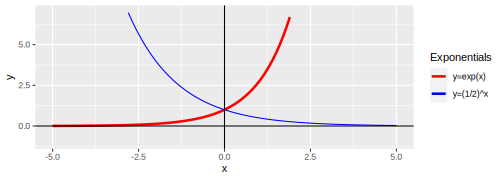
\includegraphics{fy_Alectnotes_files/figure-latex/t07-exp-graph-1.pdf}
\caption{\label{fig:t07-exp-graph}Graph of the natural logarithm function}
\end{figure}

\begin{example}
\protect\hypertarget{exm:unnamed-chunk-77}{}{\label{exm:unnamed-chunk-77} }In a circuit containing a capacitor, the \emph{instantaneous voltage} across the capacitor is given by the equation
\[\nu = V\left(1-e^{\frac{-t}{RC}}\right),\]
where \(V\) is the initial supply voltage, \(R\) is the resistance, \(C\) is the capacitance and \(t\) is the time since the initial connection of the supply voltage. If \(V=200\,\mathrm{V}\), \(R=10\,\mathrm{k}\Omega\) and \(C=20\,\mu\mathrm{F}\), calculate the time when the voltage reaches \(\nu =100\,\mathrm{V}\).
\end{example}
\begin{solution}
\iffalse{} {Solution. } \fi{}We want to make \(t\) the subject of the formula above:
\begin{align*}
\frac{\nu}{V} &=1-e^{\frac{-t}{RC}}\\
e^{\frac{-t}{RC}} &= 1-\frac{\nu}{V}\\
-\frac{t}{RC} &= \ln\left(1-\frac{\nu}{V}\right)\\
t &= -RC\ln\left(1-\frac{\nu}{V}\right)\\
\end{align*}
Hence
\begin{align*}
t&=-10\,\mathrm{k}\Omega\cdot 20\,\mu\mathrm{F}\cdot \ln\left(1-\frac{100\,\mathrm{V}}{200\,\mathrm{V}}\right)\\
&\approx 138.6\cdot 10^3\cdot 10^{-6} \,\Omega\mathrm{F}\\
&= 138.6 \,\mathrm{ms}
\end{align*}
(since \(\Omega\mathrm{F} = \mathrm{s}\)).
\end{solution}

\hypertarget{exercises-7-exponential-functions}{%
\chapter*{Exercises 7 (Exponential functions)}\label{exercises-7-exponential-functions}}
\addcontentsline{toc}{chapter}{Exercises 7 (Exponential functions)}

\begin{enumerate}
\def\labelenumi{\arabic{enumi}.}
\item
  Evaluate the following:

  \begin{enumerate}
  \def\labelenumii{\roman{enumii})}
  \tightlist
  \item
    \(y=200e^{1.75}\)
  \item
    \(y=40.8+e^2\)
  \item
    \(s=3e^{5.1}-49.8\)
  \item
    \(x=(150e^{-1.34})-(3.4e^{0.445})\)
  \item
    \(x=3.2e^3 - (6-e^{-0.8})\)
  \end{enumerate}
\item
  Calculate the value of \(x\) in each case:

  \begin{enumerate}
  \def\labelenumii{\roman{enumii})}
  \tightlist
  \item
    \(25=e^x\)
  \item
    \(34=3e^x\)
  \item
    \(268=e^{1.4x}\)
  \item
    \(94.2=e^{-3.2x}\)
  \item
    \(0.72=e^{-0.08x}\)
  \end{enumerate}
\item
  If \(T=R\ln\left(\frac{a}{a-b}\right)\), calculate \(a\) when \(T=25\), \(R=28\) and \(b=3\).
\item
  In the formula \(i=Ie^{-\frac{Rt}{L}}\), \(i=50\,\mathrm{mA}\), \(I=150\,\mathrm{mA}\) (units: miliAmperes), \(R=60\,\Omega\) (units: Ohm) and \(L=0.3\,\mathrm{H}\) (units: Henry). Determine the corresponding value of \(t\). (Recall that for units, we have \(\mathrm{H}/\Omega = \mathrm{s}\). Optional bit: This formula describes current through the inductor when discharging in an RL-circuit.)
\item
  The instantaneous charge in a capacitive circuit is given by \(q=Q\left(1-e^{-\frac{t}{RC}}\right)\). Calculate the value of \(t\) (time) when \(q=0.01\,\mathrm{C}\), \(Q=0.015\,\mathrm{C}\) (units: Coulomb), \(C=0.0001\,\mathrm{F}\) (units: Farad) and \(R=7000\,\Omega\) (units: Ohm). (Recall that for units, we have \(\Omega\cdot\mathrm{F}=\mathrm{s}\).)
\item
  From the formula \(v=V\left(1-e^{-\frac{t}{RC}}\right)\), calculate the value of \(C\) (capacitance, units: Farad) when \(v=130\,\mathrm{V}\), \(V=440\,\mathrm{V}\) (units: Volt), \(t=0.156\,\mathrm{s}\) (units: second) and \(R=44000\Omega\) (units: Ohm). (Recall that for units, we have \(\Omega\cdot\mathrm{F}=\mathrm{s}\). Optional bit: This formula describes the instantaneous voltage over a capacitor when charging in an RC-circuit.)
\item
  Plot the function \(y = 3e^{2x}\) over the range \(x = -3\) to \(x = 3\) and from the graph determine the value
  of \(y\) when \(x = 1.7\) and the value of \(x\) when \(y = 3.3\).
\item
  For values of \(x\) from \(-0.5\) to \(1.5\), plot the graph represented by the equation \(y = 10e^{2x}\).
\item
  Given the formula \(i=\frac{E}{R}\left(1-e^{-\frac{Rt}{L}}\right)\), plot the curve of \(i\) against \(t\) when \(E=300\), \(R=30\) and \(L=5\) for the range of \(t\) from \(0\) to \(0.8\). From the graph, estimate the value of \(t\) when \(i=3.2\) and also calculate the value of \(t\) using the formula to check the accuracy of the graph.
\item
  The formula \(i = 2(1 - e^{-10t})\) represents the relationship between the instantaneous current \(i\)
  (measured in Amps) and the time \(t\) (measured in seconds) in an inductive circuit. Plot a graph of \(i\)
  against \(t\) taking values of \(t\) from \(0\) to \(0.3\) at intervals of \(0.05\). From the graph determine the time
  taken for the current to increase from \(1.0\) to \(1.6\,\mathrm{A}\) and check this value by calculation.
\item
  A coil has an inductance value of \(L=2.2\,\mathrm{H}\) and a resistance \(R=15\,\Omega\). It is connected to a voltage supply with \(E=12\,\mathrm{V}\). After connection, the current \(i\) is given by \(i=\frac{E}{R}\left(1-e^{-\frac{Rt}{L}}\right)\).
  Draw a graph of the current plotted against time from the moment of connection and for the first \(0.8\) seconds. From the graph establish the time it will take for the current to reach \(50\%\) of its final value and check this value by calculation.
\item
  A coil of inductance \(L\) and resistance \(R\) are connected as shown below.
\end{enumerate}

\begin{center}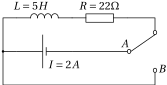
\includegraphics{t07-circuit} \end{center}

The switch is moved from contact A to contact B with the result that the current \(i\) decreases according to the equation \(i=I\left(1-e^{-\frac{Rt}{L}}\right)\). Draw the graph for this decrease plotting \(i\) against \(t\) for a time of \(300\,\mathrm{ms}\) after the switch is moved. From the plot estimate the current flowing \(158\,\mathrm{ms}\) after switching.

\emph{Solutions:}
\textbf{1.} (i) \(1151\); (ii) \(48.2\); (iii) \(442\); (iv) \(33.97\); (v) \(58.7\);
\textbf{2.} (i) \(3.2\); (ii) \(2.43\); (iii) \(3.99\); (iv) \(-1.4\); (v) \(4.12\);
\textbf{3.} \(5.1\);
\textbf{4.} \(5.5\,\mathrm{ms}\);
\textbf{5.} \(769\,\mathrm{ms}\);
\textbf{6.} \(0.00001\,\mathrm{F}\);
\textbf{9.} \(t=64\times 10^{-3}\);
\textbf{10.} \(91.9\times 10^{-3}\,\mathrm{s}\);
\textbf{11.} \(0.1\,\mathrm{s}\);
\textbf{12.} \(1\,\mathrm{A}\)

\hypertarget{long-division-and-factorisation}{%
\chapter{Long division and factorisation}\label{long-division-and-factorisation}}

\hypertarget{polynomials-and-long-division}{%
\section{Polynomials and long division}\label{polynomials-and-long-division}}

A \textbf{polynomial} is an expression of the form
\[p(x) = a_nx^n+a_{n-1}x^{n-1}+\cdots+a_1 x+a_0, \]
where \(a_0,\dots,a_n\) are constants, also called \textbf{coefficients}. Its \textbf{degree} (or \textbf{order}) is the highest occurring power of \(x\); in other words if \(a_n\neq 0\), then the degree of \(p(x)\) above is \(n\).

The low--degree polynomials have special names:

\begin{longtable}[]{@{}
  >{\centering\arraybackslash}p{(\columnwidth - 4\tabcolsep) * \real{0.29}}
  >{\centering\arraybackslash}p{(\columnwidth - 4\tabcolsep) * \real{0.18}}
  >{\raggedright\arraybackslash}p{(\columnwidth - 4\tabcolsep) * \real{0.32}}@{}}
\toprule
example polynomial & its degree & also called \\ \addlinespace
\midrule
\endhead
\(x-7\) & 1 & linear polynomial \\ \addlinespace
\(3x^2+2\) & 2 & quadratic polynomial \\ \addlinespace
\(4x^3+5x^2-3x\) & 3 & cubic polynomial \\ \addlinespace
\(-x^4+x^2-2\) & 4 & quartic polynomial \\ \addlinespace
\bottomrule
\end{longtable}

Recall long division of numbers:
\[
\begin{array}{rl}
      205&\text{ r. }18 \\[-3pt]
   21 \overline{){4323}}\kern-.2ex \\[-3pt]
      \underline{-42}\phantom{m}\\[-3pt]
      123 \\[-3pt]
      \underline{-105}\\[-3pt]
      18
  \end{array}
  \quad\quad\quad\text{or}\quad\quad\quad
  \begin{array}{rl}
  4323& \div \,\,21 = 205\text{ r. }18 \\
      \underline{-42}\phantom{m}\\[-3pt]
      123 \\[-3pt]
      \underline{-105}\\[-3pt]
      18
    \end{array}
\]
We can write this as
\[
\frac{4323}{21} = 205+\frac{18}{21}\quad\quad\text{or}\quad\quad
4323 = 205\cdot 21 + 18.
\]
In general:
\[
\frac{\text{dividend}}{\text{divisor}} = \text{quotient} + \frac{\text{remainder}}{\text{divisor}}
\]
or
\[
\text{dividend} = \text{quotient}\cdot\text{divisor} + \text{remainder}.
\]
Long division of polynomials works very similarly:
\[
\begin{array}{rl}
(x^4-x^3+x^2-3x+5)&\div\,\,\, (x-1) = x^3+x-2\quad\text{r. }3\\
\underline{-(x^4 -x^3)}\phantom{+x^2-3x+5)}&\\
0+x^2-3x\phantom{+5x)}\\
\underline{-(x^2-x)}\phantom{+5x)}\\
-2x+5\phantom{m}\\
\underline{-(-2x+2)}\phantom{)}\\
3\phantom{m}
\end{array}
\]
If we write \(p(x):=x^4-x^3+x^2-3x+5\) (for the dividend) and \(q(x):=x^3+x-2\) (for the quotient), we can write
\[
p(x) = q(x)\cdot(x-1) + 3.
\]
This holds for any \(x\), so in particular for \(x=1\) we get \(p(1) = q(1)\cdot0+3=3\).

\begin{theorem}[Remainder Theorem]
\protect\hypertarget{thm:unnamed-chunk-82}{}{\label{thm:unnamed-chunk-82} \iffalse (Remainder Theorem) \fi{} }The remainder left when a polynomial \(p(x)\) is divided by \(x-a\) is equal to \(p(a)\). In particular, \(x-a\) is a factor of \(p(x)\) if an only if \(p(a)=0\).
\end{theorem}

\begin{example}
\protect\hypertarget{exm:unnamed-chunk-83}{}{\label{exm:unnamed-chunk-83} }Determine the remainder when \(p(x)=5x^3+2x^2-6\) is divided by \(x-2\).
\end{example}
\begin{solution}
\iffalse{} {Solution. } \fi{}The remainder is \(p(2) = 5\cdot8+2\cdot4-6=42\).
\end{solution}

\begin{example}
\protect\hypertarget{exm:unnamed-chunk-85}{}{\label{exm:unnamed-chunk-85} }Divide \(3x^3-16x^2+15x+18\) by \(x-3\):
\[
\begin{array}{rl}
(3x^3-16x^2+15x+18) &\div \,\,\,(x-3) = 3x^2-7x-6\\
\underline{-(3x^3-9x^2)}\phantom{+15x+18x}\\
-7x^2 + 15x\phantom{+18x)}\\
\underline{-(-7x^2+21x)}\phantom{+18o}\\
-6x+18\phantom{x}\\
\underline{-(-6x+18)}\\
0\phantom{x}
\end{array}
\]
Thus \(3x^3-16x^2+15x+18 = (3x^2-7x-6)(x-3)\).\\
Using a quadratic formula or by inspection, we can further factorise the quadratic as \(3x^2-7x-6 = (x-3)(3x+2)\).\\
Altogether, we obtain complete factorisation
\[3x^3-16x^2+15x+18=(x-3)^2(3x+2).\]
\end{example}

\hypertarget{obtaining-the-factorisation-of-a-polynomial}{%
\section{Obtaining the factorisation of a polynomial}\label{obtaining-the-factorisation-of-a-polynomial}}

We start with a polynomial \(p(x)=x^n+a_{n-1}x^{n-1}+\cdots+a_1x+a_0\). We wish to factorise it as much as possible, ideally into linear factors.

(Note that this is a heuristic algorithm, i.e.~it may not always work. The
point is that getting a factorisation of a polynomial in the end amounts to
finding its roots --- and Abel's impossibility theorem asserts that there is no
algebraic formula that would yield the solutions of an equation \(p(x)=0\) when
degree of the polynomial \(p(x)\) is 5 or higher.)

\textbf{Step 1.} (``Guess a root.'') Calculate \(p(b)\) for divisors \(b\) of \(a_0\). When we find \(b\) such that \(p(b)=0\), we know that \(x-b\) is a factor of \(p(x)\), and we perform\dots

\textbf{Step 2.} (``Divide.'') Calculate \(q(x) := p(x)\div(x-b)\) using long division.

\textbf{Repeat.} Apply Steps 1. and 2. to the ``new'' polynomial \(q(x)\) (in place of \(p(x)\).\textbackslash{}
Note that \(q(x)\) has degree one less than the degree of \(p(x)\), so eventually
we end up with a linear polynomial, and so we are done.

\begin{example}
\protect\hypertarget{exm:unnamed-chunk-86}{}{\label{exm:unnamed-chunk-86} }Factorise \(p(x)=x^4-x^3+x^2-3x+2\).
\end{example}
\begin{solution}
\iffalse{} {Solution. } \fi{}\(p(1)=1-1+1-3+2=0\) \(\implies\) \(x-1\) is a factor of \(p(x)\). Next, we perform long division:
\[
\begin{array}{rl}
(x^4-x^3+x^2-3x+2) & \div \,\,\,(x-1) = x^3+x-2 =: q(x)\\
\underline{-(x^4-x^3)}\phantom{+x^2-3x+2x}\\
0 + x^2-3x\phantom{+2m}\\
\underline{-(x^2-x)}\phantom{+2x}\\
-2x+2\phantom{x}\\
\underline{-(-2x+2)}\\
0\phantom{x}
\end{array}
\]
Next, we now look for a root of \(q(x)\).\\
\(q(1) = 1+1-2=0\) \(\implies\) \(x-1\) is a factor of \(q(x)\). We continue by performing long division:
\[
\begin{array}{rl}
(x^3\phantom{-xm}+x-2) & \div \,\,\,(x-1) = x^2+x+1\\
\underline{-(x^3-x^2)}\phantom{x+2xx}\\
0 + x^2+x\phantom{+2m}\\
\underline{-(x^2-x)}\phantom{+2x}\\
 2x-2\phantom{x}\\
\underline{-(2x-2)}\\
0\phantom{x}
\end{array}
\]
We now try to continue by further factorising \(x^2+x+1\). However the discriminant of this quadratic is \(1-4\cdot2=-7<0\), so it can not be further factorised.\\
\emph{Answer:} \(p(x)=(x-1)^2(x^2+x+1)\).
\end{solution}

\begin{example}
\protect\hypertarget{exm:unnamed-chunk-88}{}{\label{exm:unnamed-chunk-88} }\[
\begin{array}{rl}
(x^3+5x^2-7x+3) &\div\,\,\,(x^2+2x+1) = x+3\quad\text{ rem. }-14x\\
\underline{-(x^3+2x^2+\phantom{7}x)}\phantom{+3)}\\
3x^2-8x+3\phantom{)}\\
\underline{-(3x^2+6x+3)}\\
-14x\phantom{+3m}
\end{array}
\]
\end{example}

\begin{example}
\protect\hypertarget{exm:unnamed-chunk-89}{}{\label{exm:unnamed-chunk-89} }The polynomial \(p(x)=6x^3-23x^2+ax+b\) leaves remainder \(11\) when divided by \(x-3\) and remainder \(-21\) when divided by \(x+1\).

\begin{enumerate}
\def\labelenumi{(\roman{enumi})}
\tightlist
\item
  Show that \(a\) and \(b\) satisfy the equations \(3a+b=56\), \(-a+b=8\).
\item
  Solve the simultaneous equations above.
\item
  Show that \(x-2\) is a factor of \(p(x)\).
\item
  Factorise \(p(x)\).
\item
  Determine the roots of \(p(x)\).
\end{enumerate}
\end{example}

\begin{enumerate}
\def\labelenumi{(\roman{enumi})}
\item
  Deriving the equations:

  \begin{itemize}
  \tightlist
  \item
    \(p(x)\) leaves a remainder of \(11\) when divided by \(x-3\)\\
    \(\iff\) \(p(3)=11\) \hfill~{(by Remainder Theorem)}\\
    \(\iff\) \(6\cdot 27-23\cdot 9+3a+b = 11\)\\
    \(\iff\) \(3a+b=56\) ~ ~ ~ (A)
  \item
    \(p(x)\) leaves a remainder of \(-21\) when divided by \(x+1\)\\
    \(\iff\) \(p(-1)=-21\) \hfill~{(by Remainder Theorem)}\\
    \(\iff\) \(-6-23-a+b=-21\)\\
    \(\iff\) \(-a+b=8\) ~ ~ ~ (B)
  \end{itemize}
\item
  From (A): \(b=56-3a\).\\
  Substitute into (B): \(-a+56-3a = 8\)\\
  \(\iff\) \(4a=48\)\\
  \(\iff\) \(a=12\).
  Substitute back into (B): \(-12+b=8\)\\
  \(\iff\) \(b=20\).
\item
  From (ii): \(p(x)=6x^3-23x^2+12x+20\).\\
  \(p(2)=6\cdot8 - 23\cdot 4+12\cdot2+20=48-92+24+20=0\), so \(x-2\) is a factor of \(p(x)\) by Remainder Theorem.
\item
  We start by long division by the factor we already know from (iii).
  \[
  \begin{array}{rl}
  (6x^3-23x^2+12x+20) &\div\,\,\,(x-2) = 6x^2-11x-10\\
  \underline{-(6x^3-12x^2)}\phantom{+12x+20)}\\
  -11x^2+12x\phantom{+20m}\\
  \underline{-(-11x^2+22x)}\phantom{+20)}\\
  -10x+20\phantom{)}\\
  \underline{-(-10x+20)}\\
  0\phantom{)}
  \end{array}
  \]
  By inspection: \(6x^2-11x-10=(2x-5)(3x+2)\).
  So altogether \(p(x)=(x-2)(2x-5)(3x+2)\).
\item
  From (iv): the roots of \(p(x)\) are \(x=2\), \(x=\frac{5}{2}\) and \(x=-\frac{2}{3}\).
\end{enumerate}

\hypertarget{exercises-8-long-division-and-the-remainder-theorem}{%
\chapter*{Exercises 8 (Long division and the Remainder theorem)}\label{exercises-8-long-division-and-the-remainder-theorem}}
\addcontentsline{toc}{chapter}{Exercises 8 (Long division and the Remainder theorem)}

\begin{enumerate}
\def\labelenumi{\arabic{enumi}.}
\item
  Show that \(x - 3\) is a factor of \(6x^3 - 19x^2 + x + 6\) and hence determine the other factors.
\item
  Given that \(x = 0.25\) is one root which satisfies the equation \(4x^3 + 3x^2 - 5x + 1 = 0\). Determine the other roots.
\item
  Establish the remainder when:

  \begin{enumerate}
  \def\labelenumii{\roman{enumii})}
  \tightlist
  \item
    \(x - 4\) is divided into \(24x^4 - 5x^3 + 3x\)
  \item
    \(x + 5\) is divided into \(4x^3 + 25x^2 + 20x - 25\)
  \item
    \(x - 2\) is divided into \(12x^3 + x^2 - 38x - 24\)
  \end{enumerate}
\item
  Determine the quotient and remainder when:

  \begin{enumerate}
  \def\labelenumii{\roman{enumii})}
  \tightlist
  \item
    \(x - 2\) is divided into \(x^3 + 14x^2 + 56x + 14\)
  \item
    \(x + 2\) is divided into \(4x^4 + 3x^2 - 21x + 4\)
  \end{enumerate}
\item
  Solve for \(x\): \(2x^3-5x^2-x+6=0\).
\item
  The power of a flat belt is given by the formula \(P = Av + Bv^3\), where \(v\) is the linear velocity of the belt and \(A\) and \(B\) are constants. Given that \(A = 12\) and \(B = -1\), determine the value of the velocity when \(P = 16\).
\item
  The value of the magnetic field at a given point due to the presence of two magnets of equal moment, \(M\), is given by
  \[F=\frac{2M}{d_1^3}-\frac{2M}{d_2^3}, \tag{1}\]
  where \(d_1\) and \(d_2\) are the distances of the magnets from the given point. Show that the field may be expressed as
  \[F=2M\left(\frac{(d_2-d_1)(d_2^2+d_1d_2+d_1^2)}{d_1^3d_2^3}\right). \tag{2}\]
  (Hint: Starting with the equation (1), add the fractions and then find a factor for the numerator.)
\item
  Use algebraic long division to find the quotient and the remainder for the following:

  \begin{enumerate}
  \def\labelenumii{\alph{enumii})}
  \tightlist
  \item
    \(x^3 + 2x^2 – x – 2\) divided by \(x – 1\)
  \item
    \(2x^3 + 9x^2 – 4x – 21\) divided by \(2x – 3\)
  \item
    \(x^4 + x^3 + 7x – 3\) divided by \(x^2 – x + 3\)
  \item
    \(6x^4 + 14x^3 – 9x^2 – 7x + 3\) divided by \(2x^2 – 1\)
  \end{enumerate}
\item
  Find the quotient and remainder for:

  \begin{enumerate}
  \def\labelenumii{\alph{enumii})}
  \tightlist
  \item
    \(\dfrac{x^2+6x-2}{x^2+4x+1}\)
  \item
    \(\dfrac{2x^2+5}{x^2+1}\)
  \item
    \(\dfrac{5x^2+2x-11}{x^2+x-2}\)
  \item
    \(\dfrac{x^3-5x^2+9x-7}{x^2-2x+8}\)
  \end{enumerate}
\item
  Use the remainder theorem to find the remainder when:

  \begin{enumerate}
  \def\labelenumii{\alph{enumii})}
  \tightlist
  \item
    \(6x^3 + 7x^2 - 15x + 4\) is divided by \((x - 1)\)
  \item
    \(2x^3 - 3x^2 + 5x + 4\) is divided by \((x + 1)\)
  \item
    \(x^3 - 7x^2 + 6x + 1\) is divided by \((x - 3)\)
  \item
    \(5 + 6x + 7x^2 - x^3\) is divided by \((x + 2)\)
  \item
    \(x^4 - 3x^3 + 2x^2 + 5\) is divided by \((x - 1)\)
  \end{enumerate}
\item
  Factorise:

  \begin{enumerate}
  \def\labelenumii{\alph{enumii})}
  \tightlist
  \item
    \(x^3 - 2x^2 - 5x + 6\)
  \item
    \(2x^3 + 7x^2 - 7x - 12\)
  \item
    \(2x^3 + 3x^2 - 17x + 12\)
  \item
    \(6x^3 - 5x^2 - 17x + 6\)
  \item
    \(2x^4 + 7x^3 - 17x^2 -7x + 15\)
  \item
    \(6x^4 + 31x^3 + 57x^2 + 44x + 12\)
  \end{enumerate}
\item
  Given that \(x + 2\) is a factor of \(2x^3 + 6x^2 + bx - 5\), find the value of \(b\) and then find the remainder when the expression is divided by \((2x - 1)\).
\item
  The expression \(3x^3 + 2x^2 - bx + a\) is exactly divisible by \((x - 1)\), but leaves a remainder of \(10\) when divided by \((x + 1)\). Find the values of \(a\) and \(b\).
\item
  The expression \(8x^3 - 4x^2 + ax + b\) gives a remainder of \(-19\) when divided by \((x + 1)\) and a remainder of \(2\) when divided by \((2x - 1)\). Find the values of \(a\) and \(b\).
\end{enumerate}

\emph{Solutions:}
\textbf{1.} \((x-3)(3x-2)(2x+1)\);
\textbf{2.} \(-1.618\), \(0.618\);
\textbf{3.} (i) \(5836\); (ii) \(0\); (iii) \(0\);
\textbf{4.} (i) \(Q=x^2+16x+88\), \(r=190\); (ii) \(Q=4x^3-8x^2+19x-59\), \(r=122\);
\textbf{5.} \(2,3/2,-1\);
\textbf{6.} \(v=2\) (twice), or \(v=-4\);
\textbf{8.} (a) \(x^2+3x+2\) rem \(0\); (b) \(x^2+6x+7\) rem \(0\); (c) \(x^2+2x-1\) rem \(0\); (d) \(3x^2+7x-3\) rem \(0\);
\textbf{9.} (a) \(1\) rem \(2x-3\); (b) \(2\) rem \(3\); (c) \(5\) rem \(-3x-1\); (d) \(x-3\) rem \(-5x+17\);
\textbf{10.} (a) \(2\); (b) \(-6\); (c) \(-17\); (d) \(29\); (e) \(5\);
\textbf{11.} (a) \((x -1)(x - 3)(x + 2)\); (b) \((2x - 3)(x + 4)(x + 1)\); (c) \((2x - 3)(x + 4)(x - 1)\); (d) \((3x - 1)(2x + 3)(x - 2)\); (e) \((x + 1)(x - 1)(2x - 3)(x + 5)\); (f) \((x + 1)(x + 2)(3x + 2)(2x + 3)\);
\textbf{12.} \(b = 3/2\) and the reminder when divided by \((2x-1)\) is \(-5/2\);
\textbf{13.} \(a=3, b=8\);
\textbf{14.} \(a=6,b=-1\)

\hypertarget{partial-fractions}{%
\chapter{Partial fractions}\label{partial-fractions}}

A \textbf{rational function} is a quotient of two polynomials, i.e.~an expression of the form \(\dfrac{p_1(x)}{p_2(x)}\), where both \(p_1(x)\) and \(p_2(x)\) are polynomials, and \(p_2(x)\neq0\).

For example: \(\dfrac{5x+7}{3x^2+5}\), \(\dfrac{5x^2-4x+3}{x-7}\), \ldots{}

Long division of polynomials allows us to write \(\dfrac{p_1(x)}{p_2(x)}\) in the form
\[
\frac{p_1(x)}{p_2(x)} = q(x) + \frac{r(x)}{p_2(x)},
\]
where \(q(x)\) and \(r(x)\) are polynomials and the degree of \(r(x)\) is less than
the degree of \(p_2(x)\).

The aim of ``partial fractions'': simplify \(\dfrac{r(x)}{p_2(x)}\) further.

\textbf{First} factorise the denominator \(p_2(x)\) (completely\footnote{When the coefficients of a polynomial are real numbers, it is always possible to factorise it into a product of factors, each of which is either linear, or an irreducible quadratic. (This is a consequence of the Fundamental Theorem of Algebra.)}).

\textbf{Then}, every rational function of the type as in the left--hand column can be split
into \textbf{partial fractions} as given in the right--hand column:

\begin{longtable}[]{@{}
  >{\raggedright\arraybackslash}p{(\columnwidth - 6\tabcolsep) * \real{0.09}}
  >{\raggedleft\arraybackslash}p{(\columnwidth - 6\tabcolsep) * \real{0.37}}
  >{\raggedright\arraybackslash}p{(\columnwidth - 6\tabcolsep) * \real{0.03}}
  >{\raggedright\arraybackslash}p{(\columnwidth - 6\tabcolsep) * \real{0.50}}@{}}
\toprule
\endhead
Type I & \(\dfrac{Px+Q}{(ax+b)(cx+d)}\) & = & \(\dfrac{A}{ax+b}+\dfrac{B}{cx+d}\) \\ \addlinespace
Type II & \(\dfrac{Px+Q}{(ax+b)^2}\) & = & \(\dfrac{A}{ax+b}+\dfrac{B}{(ax+b)^2}\) \\ \addlinespace
Type III & \(\dfrac{Px^2+Qx+R}{(ax+b)^2(cx+d)}\) & = & \(\dfrac{A}{ax+b}+\dfrac{B}{(ax+b)^2}+\dfrac{C}{cx+d}\) \\ \addlinespace
Type IV & \(\dfrac{Px^2+Qx+R}{(ax^2+bx+c)(dx+e)}\) & = & \(\dfrac{Ax+B}{ax^2+bx+c}+\dfrac{C}{dx+e}\) \\ \addlinespace
\bottomrule
\end{longtable}

Note: It is a Theorem that the above actually works --- these are equations which work for all values of \(x\) simultaneously! It is not proved here though.

\begin{example}
\protect\hypertarget{exm:unnamed-chunk-92}{}{\label{exm:unnamed-chunk-92} }Split \(\dfrac{-4x+15}{(x+2)(x-1)}\) into partial fractions.
\end{example}

\begin{solution}
\iffalse{} {Solution. } \fi{}First, note that the degree of the numerator is less than the degree of the denominator, so we do not need to perform any long division.

Second, the denominator is already factored as much as possible (into linear factors). We see that it is ``Type I'', so we want to find \(A\) and \(B\) such that
\[
\frac{-4x+15}{(x+2)(x-1)} = \frac{A}{x+2}+\frac{B}{x-1}
\]
Multiplying both sides by \((x+2)(x-1)\), we arrive at\\
\(-4x+15 = A(x-1)+B(x+2)\).\\
Let \(x=1\). Then \(-4+15 = A\cdot 0+B\cdot 3\) \(\implies\) \(B=\frac{11}{3}\).\\
Let \(x=-2\). Then \(8+15=A(-3)+B\cdot 0\) \(\implies\) \(A=-\frac{23}{3}\).\\
\emph{Answer:}
\(\dfrac{-4x+15}{(x+2)(x-1)} = -\dfrac{23}{3(x+2)}+\dfrac{11}{3(x-1)}.\)
\end{solution}

\begin{example}
\protect\hypertarget{exm:unnamed-chunk-94}{}{\label{exm:unnamed-chunk-94} }Split \(\dfrac{5x^2-3x+2}{(x-3)^2(x+2)}\) into partial fractions.
\end{example}

\begin{solution}
\iffalse{} {Solution. } \fi{}(Type III.) We want to find \(A,B,C\) such that
\[
\frac{5x^2-3x+2}{(x-3)^2(x+2)}=\frac{A}{x-3}+\frac{B}{(x-3)^2}+\frac{C}{x+2}.
\]
\(\iff\) \(5x^2-3x+2 = A(x-3)(x+2)+B(x+2)+C(x-3)^2\).\\
Let \(x=-2\). Then \(5\cdot 4-3(-2)+2 = C\cdot(-5)^2\) \(\implies\) \(C=\frac{28}{25}\).\\
Let \(x=3\). Then \(5\cdot 9-3\cdot 3+2 = B\cdot 5\) \(\implies\) \(B=\frac{38}{5}\).\\
Equating coefficients of \(x^2\) gives \(5=A+C\) \(\implies\) \(A=5-C=5-\frac{28}{25}=\frac{97}{25}\).\\
\emph{Answer:}
\(\dfrac{5x^2-3x+2}{(x-3)^2(x+2)}=\dfrac{97}{25(x-3)}+\dfrac{38}{5(x-3)^2}+\dfrac{28}{25(x+2)}.\)
\end{solution}

\begin{example}
\protect\hypertarget{exm:unnamed-chunk-96}{}{\label{exm:unnamed-chunk-96} }Split \(\dfrac{2x+5}{(x^2+x+1)(x+3)}\) into partial fractions.
\end{example}

\begin{solution}
\iffalse{} {Solution. } \fi{}(Type IV.) We want to find \(A,B,C\) such that
\[\dfrac{2x+5}{(x^2+x+1)(x+3)}=\dfrac{Ax+B}{x^2+x+1}+\dfrac{C}{x+3}.\]
\(\iff\) \(2x+5=(Ax+B)(x+3)+C(x^2+x+1)\).\\
Let \(x=-3\). Then \(2\cdot(-3)+5=C\cdot(9-3+1)\) \(\implies\) \(C=-\frac17\).\\
Equating coefficients of \(x^2\) gives \(0=A+C\) \(\implies\) \(A=\frac17\).\\
Equating constant coefficients gives \(5=3B+C\) \(\implies\) \(B=\frac{5-C}{3}=\frac{12}7\).\\
\emph{Answer:}
\(\dfrac{2x+5}{(x^2+x+1)(x+3)}=\dfrac{x+12}{7(x^2+x+1)}-\dfrac{1}{7(x+3)}.\)
\end{solution}

\hypertarget{exercises-9-partial-fractions}{%
\chapter*{Exercises 9 (Partial fractions)}\label{exercises-9-partial-fractions}}
\addcontentsline{toc}{chapter}{Exercises 9 (Partial fractions)}

Express the following fractions in terms of partial fractions:

\begin{enumerate}
\def\labelenumi{\roman{enumi})}
\tightlist
\item
  \(\dfrac{x-4}{(x-2)(x+1)}\)
\item
  \(\dfrac{3x+2}{(x+1)(x-5)}\)
\item
  \(\dfrac{4x^2-2}{(x^2+3)(x-2)}\)
\item
  \(\dfrac{3x^2+1}{(x^2+4)(3x-1)}\)
\item
  \(\dfrac{4x^2-3x+2}{(x-2)(2+x^2)}\)
\item
  \(\dfrac{x-6}{(x-3)^2(x+1)}\)
\item
  \(\dfrac{6x-7}{(x-5)(x-4)^2}\)
\item
  \(\dfrac{2x^2+5x-3}{(x-1)(x-3)}\)
\item
  \(\dfrac{3x^3+x^2+2x-4}{(x-2)^2(x-1)}\)
\item
  \(\dfrac{2x^2+5x-3}{(x+1)(2x-3)(x-4)}\)
\end{enumerate}

\emph{Solutions:}

\begin{enumerate}
\def\labelenumi{\roman{enumi})}
\tightlist
\item
  \(\dfrac{-2}{3(x-2)}+\dfrac 5{3(x+1)}\)
\item
  \(\dfrac 1{6(x+1)}+\dfrac{17}{6(x-5)}\)
\item
  \(\dfrac{2x+4}{x^2+3}+\dfrac 2{x-2}\)
\item
  \(\dfrac{33x+11}{37(x^2+4)}+\dfrac{12}{37(3x-1)}\)
\item
  \(\dfrac{2x+1}{2+x^2}+\dfrac 2{x-2}\)
\item
  \(\dfrac{-3}{4(x-3)^2}+\dfrac 7{16(x-3)}-\dfrac 7{16(x+1)}\)
\item
  \(\dfrac{-17}{(x-4)^2}-\dfrac{23}{x-4}+\dfrac{23}{x-5}\)
\item
  \(2-\dfrac 2{x-1}+\dfrac{15}{x-3}\)
\item
  \(3+\dfrac{28}{(x-2)^2}+\dfrac{14}{x-2}+\dfrac 2{x-1}\)
\item
  \(\dfrac{-6}{25(x+1)}-\dfrac{36}{25(2x-3)}+\dfrac{49}{25(x-4)}\)
\end{enumerate}

\hypertarget{arithmetic-and-geometric-progressions}{%
\chapter{Arithmetic and geometric progressions}\label{arithmetic-and-geometric-progressions}}

\hypertarget{arithmetic-progressions}{%
\section{Arithmetic progressions}\label{arithmetic-progressions}}

An \textbf{arithmetic progression (AP)} is a (finite or infinite) sequence of numbers
\[
a_1,a_2,a_3,\dots
\]
such that the difference between consecutive terms is a constant (also called the \textbf{common difference}) \(d\). In other words,
\[
d=a_2-a_1=a_3-a_2=a_4-a_3=\dots.
\]
For example:

\begin{itemize}
\tightlist
\item
  \(1,3,5,7,\dots\) \quad (\(d=2\))
\item
  \(3,1,-1,-3,-5,\dots\) \quad (\(d=-2\))
\end{itemize}

We have
\begin{align*}
    a_2&=a_1+d\\
    a_3&=a_2+d=a_1+2d \\
    a_4&=a_3+d=a_1+3d
\end{align*}
In general: \fbox{\(a_n = a+(n-1)d\)} where \(a=a_1\).

\begin{theorem}
\protect\hypertarget{thm:unnamed-chunk-100}{}{\label{thm:unnamed-chunk-100} }The sum \(S_n\) of the first \(n\) terms of an AP with the first term \(a\) and the common difference \(d\) is given by
\[
\boxed{S_n=\frac{n}2\left(2a+(n-1)d\right)}
\]
\end{theorem}

\emph{Proof (non-examinable):}
\[
\begin{array}{ccccccccc}
S_n &=& a & + & (a+d) & + & \dots & + & (a+(n-1)d) \\
S_n &=& (a+(n-1)d) & + & (a+(n-2)d) & + &  \dots & + & a\\
\implies \\
2S_n & = & (2a+(n-1)d) & + & (2a+(n-1)d) & + & \dots & + & (2a+(n-1)d)\\
& = & n(2a+(n-1)d)
\end{array}
\]
The ``\(\implies\)'' step is by summing the two previous equations ``vertically''. The last step holds as there are \(n\) summands, each of them equal to \(2a+(n-1)d\)).

Hence \(S_n = \frac{n}{2}(2a+(n-1)d)\).

\begin{example}
\protect\hypertarget{exm:unnamed-chunk-101}{}{\label{exm:unnamed-chunk-101} }Determine the sum \(S_{20}\) of the first \(20\) terms of the arithmetic progression: \(10, 6, 2, -2, \dots\).
\end{example}

\begin{solution}
\iffalse{} {Solution. } \fi{}\(a=10\), \(d=-4\), \(n=20\)\\
\(\implies\) \(S_{20}=\frac{20}{2}(2\cdot 10+ 19\cdot(-4))\) \(=10(20-76)=-560\).
\end{solution}

\begin{example}
\protect\hypertarget{exm:unnamed-chunk-103}{}{\label{exm:unnamed-chunk-103} }The sum \(S_8\) of the first \(8\) terms of an AP is \(90\), and its first term is \(6\). What is the common difference?
\end{example}

\begin{solution}
\iffalse{} {Solution. } \fi{}\(90=S_8=\frac{8}{2}(2\cdot 6 + 7\cdot d)\)\\
\(\implies\) \(90=4(12+7d)\)\\
\(\implies\) \(\frac{90}{4}-12=7d\)\\
\(\implies\) \(d=\frac{42}{28}=\frac32=1.5\).
\end{solution}

\begin{example}
\protect\hypertarget{exm:unnamed-chunk-105}{}{\label{exm:unnamed-chunk-105} }How many terms of the AP \(3,6,9,\dots\) must be taken so that their sum is \(135\)?
\end{example}

\begin{solution}
\iffalse{} {Solution. } \fi{}\(a=3\), \(d=3\), \(S_n=135\), \(n=?\)\\
\(\implies\) \(135 = S_n = \frac{n}{2}(2\cdot 3+(n-1)\cdot 3)\)\\
\(\implies\) \(270 = 3n^2 + 3n\)\\
\(\implies\) \(n^2+n-90 = 0\)\\
\(\implies\) \((n+10)(n-9)=0\)\\
\(\implies\) \(n=9\) (since \(n\) must be positive).
\end{solution}
\#\# Geometric progressions

A \textbf{geometric progression (GP)} is a (finite or infinite) sequence of numbers
\[
a_1,a_2,a_3,\dots
\]
such that the quotient of the consecutive terms is a constant (also called the \textbf{common ratio}) \(r\). In other words,
\[
r = \frac{a_2}{a_1} = \frac{a_3}{a_2} = \frac{a_4}{a_3} = \dots
\]
For example:

\begin{itemize}
\tightlist
\item
  \(1,\frac12,\frac14,\frac18,\dots\) \quad (\(r=\frac12\))
\item
  \(2,-6,18,-54,\dots\) \quad (\(r=-3\))
\end{itemize}

We have: \(a_2=a_1r\), ~ \(a_3=a_2r = a_1r^2\), ~ \(a_4=a_3r=a_1r^3\), \dots

In general: \fbox{\(a_n=a\cdot r^{n-1}\)} where \(a=a_1\).

\begin{theorem}
\protect\hypertarget{thm:unnamed-chunk-107}{}{\label{thm:unnamed-chunk-107} }The sum \(S_n\) of the first \(n\) terms of a GP with the first
term \(a\) and the common ratio \(r\) is given by
\[
\boxed{S_n = a\cdot \frac{1-r^n}{1-r}}
\]
In particular, if \(-1<r<1\), then the sum \(S_\infty\) of all (infinitely many) terms is \(S_\infty = a\cdot\dfrac{1}{1-r}\). (The sum of an infinite GP is also called \textbf{geometric series}.)
\end{theorem}

\emph{Proof (non--examinable):}
\begin{align*}
    (1-r)S_n &= (1-r)(a+ar+\dots+ar^{n-1})\\
     &= (a+ar+\dots+ar^{n-1}) - (ar + ar^2 +\dots +ar^n) \\
     &= a-ar^n = a(1-r^n) \qquad\text{(everything else cancels)}
\end{align*}
Thus \(S_n = a\frac{1-r^n}{1-r}\).\\
Now if \(-1<r<1\), then \(\lim_{n\to\infty}r^n=0\). So \(S_\infty=\lim_{n\to\infty}S_n = a\frac{1}{1-r}\).

\begin{example}
\protect\hypertarget{exm:unnamed-chunk-108}{}{\label{exm:unnamed-chunk-108} }Determine the sum \(S_7\) of the first \(7\) terms of the geometric progession \(4,-8,16,\dots\)
\end{example}

\begin{solution}
\iffalse{} {Solution. } \fi{}\(a=4\), \(r=-2\), \(n=7\)\\
\(\implies\) \(S_7=4\dfrac{1-(-2)^7}{1-(-2)}=4\cdot\dfrac{129}3 = 172\).
\end{solution}

\begin{example}
\protect\hypertarget{exm:unnamed-chunk-110}{}{\label{exm:unnamed-chunk-110} }A GP is given by \(\dfrac14,\dfrac1{16},\dfrac1{64},\dots\). Determine \(S_\infty\).
\end{example}

\begin{solution}
\iffalse{} {Solution. } \fi{}\(a=\frac14\), \(r=\frac14\)\\
\(\implies\) \(S_\infty = \dfrac{1}{4}\cdot\dfrac{1}{1-\frac14}= \dfrac{1}{4}\cdot\dfrac{1}{\frac{3}{4}}=\dfrac{1}{3}\).
\end{solution}

\hypertarget{exercises-10-arithmetic-and-geometric-progressions}{%
\chapter*{Exercises 10 (Arithmetic and geometric progressions)}\label{exercises-10-arithmetic-and-geometric-progressions}}
\addcontentsline{toc}{chapter}{Exercises 10 (Arithmetic and geometric progressions)}

\begin{enumerate}
\def\labelenumi{\arabic{enumi}.}
\item
  For the two progressions below, determine the \(20^{\mathrm{th}}\) term:

  \begin{enumerate}
  \def\labelenumii{\roman{enumii})}
  \tightlist
  \item
    \(3,\,7.5,\,18.75,\dots\)
  \item
    \(6,\,18,\,30,\dots\)
  \end{enumerate}
\item
  Determine the common difference for an AP where the sum for the first 10 terms of the progression is \(233.75\), given that the first term is \(6.5\).
\item
  How many terms of the progression \(4,10,16,\dots\) must be taken so that the sum is equal to \(602\)?
\item
  A machine is required to have 5 speeds, the lowest being 60 rev/min and the highest 680 rev/min. State the complete range of speeds i) in AP and ii) in GP.
\item
  A drilling machine has 10 speeds arranged in GP and operates at a surface cutting speed of \(15\,\mathrm{m/s}\). The smallest drill bit has diameter \(6\,\mathrm{mm}\) and the largest drill bit has diameter \(18\,\mathrm{mm}\). Determine the complete range of speeds. (Speed in \(\mathrm{rev}\cdot\mathrm{s}^{-1}\) = surface cutting speed in \(\mathrm{m}\cdot\mathrm{s}^{-1}/\)drill bit circumference in \(\mathrm{m}\).)
\item
  A tie rod \(5\,\mathrm{m}\) long is made such that the cross-sectional areas at equal distances are a geometric progression. The area at the smaller end is \(10\,\mathrm{mm}^2\) whilst the area one tenth of the way down the rod is \(25\,\mathrm{mm}^2\). Calculate the area of the cross section at the larger end.
\item
  A body falling freely falls \(4.9\,\mathrm{m}\) in the \(1^{\mathrm{st}}\) second, \(14.7\,\mathrm{m}\) in the \(2^{\mathrm{nd}}\) second, \(24.5\,\mathrm{m}\) in the \(3^{\mathrm{nd}}\) second and so on. Determine:

  \begin{enumerate}
  \def\labelenumii{\alph{enumii})}
  \tightlist
  \item
    How far it falls in the \(10^{\mathrm{th}}\) second.
  \item
    The total distance fallen in \(10\) seconds.
  \end{enumerate}
\item
  If £50 is saved in a certain year and each year thereafter £5 more is saved than in the previous year, after how many years will the total equal £1950, excluding any interest?
\end{enumerate}

\emph{Solutions:}
\textbf{1.} (i) \(109\times 10^6\); (ii) \(234\);
\textbf{2.} \(d=3.75\);
\textbf{3.} \(14\);
\textbf{4.} (i) \(60,215,370,525,680\); (ii) \(60,110,202,371,680\);
\textbf{5.} \(265,299,338,382,432,488,552,623,704,796\);
\textbf{6.} \(95\times 10^3\,\mathrm{mm}^2\);
\textbf{7.} (a) \(93.1\,\mathrm{m}\); (b) \(490\,\mathrm{m}\);
\textbf{8.} \(20\) years

\hypertarget{binomial-theorem}{%
\chapter{Binomial Theorem}\label{binomial-theorem}}

\hypertarget{pascals-triangle}{%
\section{Pascal's triangle}\label{pascals-triangle}}

Binomial Theorem gives a formula for \((a+b)^n\).
First few:

\begin{itemize}
\tightlist
\item
  \((a+b)^2 = a^2+2ab+b^2\)
\item
  \((a+b)^3 = (a^2+2ab+b^2)(a+b) = a^3+3a^2b+3ab^2+b^3\)
\item
  \((a+b)^4 = \dots = a^4+4a^3b+6a^2b^2 + 4ab^3 + b^4\)
\end{itemize}

In general:
\[
(a+b)^n = C_{n,0}\cdot a^n + C_{n,1}\cdot a^{n-1}b + C_{n,2}\cdot a^{n-2}b^2 + \dots + C_{n,n-1}\cdot ab^{n-1} + C_{n,n}\cdot b^n
\]
for some coefficients \(C_{n,0},C_{n,1},\dots,C_{n,n}\). ``Extrapolating'' from the examples above, we can ``guess'':
\begin{align*}
    C_{n,0} &= C_{n,n} = 1\\
    C_{n,1} &= C_{n,n-1} = n\\
    C_{n,k} &= C_{n-1,k-1}+C_{n-1,k}
\end{align*}

The two rules: \(C_{n,0}=C_{n,n}=1\) and \(C_{n,k}=C_{n-1,k-1}+C_{n-1,k}\) are the building laws for \textbf{Pascal's triangle}:
\[
\begin{array}{cccccccccccccc}
    &  &  &  &  &  &  &1 &  &  &  &  &  &   \\
    &  &  &  &  &  &1 &  &1 &  &  &  &  &   \\
    &  &  &  &  &1 &  &2 &  &1 &  &  &  &   \\
    &  &  &  &1 &  &3 &  &3 &  &1 &  &  &   \\
    &  &  &1 &  &4 &  &6 &  &4 &  &1 &  &   \\
    &  &1 &  &5 &  &10&  &10&  &5 &  &1 &   \\
    &1 &  &6 &  &15&  &20&  &15&  &6 &  &1  \\
    &  &  &  &  &  &  &\vdots&  &  &  &  &  &   \\
\end{array}
\]
\begin{example}
\protect\hypertarget{exm:unnamed-chunk-114}{}{\label{exm:unnamed-chunk-114} }\((a+b)^6 = a^6 + 6 a^5b + 15 a^4b^2 + 20 a^3b^3 + 15 a^2b^4 + 6 ab^5 + b^6\).
\end{example}
\begin{example}
\protect\hypertarget{exm:unnamed-chunk-115}{}{\label{exm:unnamed-chunk-115} }\begin{align*}(a+2x)^4 &= a^4 + 4a^3(2x) + 6a^2(2x)^2 + 4a(2x)^3+(2x)^4\\
&= a^4 +8a^3x+24a^2x^2+32ax^3+16x^4.
\end{align*}
\end{example}

\begin{example}
\protect\hypertarget{exm:unnamed-chunk-116}{}{\label{exm:unnamed-chunk-116} }Expand \((1.005)^4\) to four decimal places (4 d.p).
\end{example}
\begin{solution}
\iffalse{} {Solution. } \fi{}\begin{align*}
(1.005)^4 &= (1+0.005)^4\\
&= 1+ 4\cdot 0.005 + 6\cdot (0.005)^2 + \underbrace{4\cdot(0.005)^3 + (0.005)^4}_{\text{do not contribute to 4 d.p.}}\\
&= 1+0.02 + 0.00015 + \dots \\
&\approx 1.0202\quad\quad\text{(to 4 d.p.)}
\end{align*}
\end{solution}

\hypertarget{binomial-coefficients}{%
\section{Binomial coefficients}\label{binomial-coefficients}}

For a positive integer \(m\), define \textbf{\(m\) factorial}, denoted ``\(m!\)'', as
\(m!=1\cdot2\cdot 3\cdots (m-1)\cdot m\);\\
and declare that \(0!=1\).

\begin{theorem}
\protect\hypertarget{thm:unnamed-chunk-118}{}{\label{thm:unnamed-chunk-118} }\(\boxed{C_{n,k} = \dfrac{n!}{k!\cdot (n-k)!}}\)
\end{theorem}

\emph{Note:} The number \(C_{n,k}\) is also denoted by \(\displaystyle{n\choose k}\), read ``\(n\) choose \(k\)'\,'\footnote{This is because it also computes the number of ways one can choose \(k\) objects out of \(n\).}.

\emph{Proof (non--examinable):} To argue that the formula ``works correctly'', it suffices to check that the number above satisfies the laws defining Pascal's triangle.

That \(C_{n,0}=C_{n,n}=1\) is clear.

Now checking that \(C_{n,k}=C_{n-1,k-1}+C_{n-1,k}\):
\[
\begin{matrix}
    \dfrac{n!}{k!(n-k)!} &\stackrel{?}{=} & \dfrac{(n-1)!}{(k-1)!(n-k)!} & + & \dfrac{(n-1)!}{k!(n-1-k)!}\\
                        & & = & & = \\
                        & & \dfrac{k}{n}\cdot\dfrac{n!}{k!(n-k)!} & + & \dfrac{n-k}{n}\cdot \dfrac{n!}{k!(n-k)!}
\end{matrix}
\]
This finishes the proof.

Let us analyse the formula: observe that \(C_{n,k} = \dfrac{n(n-1)(n-2)\cdots(n-k+1)}{1\cdot 2\cdot 3 \cdots k}\).

We will use this expression as a \emph{definition} for \(C_{n,k}\) when \(n\) is negative or a fraction.

\begin{theorem}
\protect\hypertarget{thm:unnamed-chunk-119}{}{\label{thm:unnamed-chunk-119} }If \(-1<x<1\), then the right hand side of
\begin{align*}
    (1+x)^n &= C_{n,0}+C_{n,1}x+C_{n,2}x^2 + C_{n,3}x^3 + \dots\\
            &= 1+ nx + \frac{n(n-1)}{2}x^2 + \frac{n(n-1)(n-2)}{6} x^3 + \dots
\end{align*}
converges\footnote{``Converges'' is a mathematical term that you will learn more precisely later on; the meaning here is roughly that ``for each \(x\), the infinite sum \emph{does} describe a well-defined and unique number, and we get better and better approximations to it by adding up more and more terms of the infinite series''.} and this equality is valid also when \(n\) is negative or a fraction.
\end{theorem}

\begin{example}
\protect\hypertarget{exm:unnamed-chunk-120}{}{\label{exm:unnamed-chunk-120} }\(\dfrac{1}{1+x} = (1+x)^{-1}\) \(=1-x+x^2-x^3+x^4 \mp\cdots\)
\end{example}

\begin{example}
\protect\hypertarget{exm:unnamed-chunk-121}{}{\label{exm:unnamed-chunk-121} }\(\dfrac{1}{1-x} = (1-x)^{-1} = 1+x+x^2+x^3+\dots\)
\end{example}

\begin{example}
\protect\hypertarget{exm:unnamed-chunk-122}{}{\label{exm:unnamed-chunk-122} }Expand \(\dfrac{1}{(1+x)^3}\) up to the term in \(x^4\).
\end{example}
\begin{solution}
\iffalse{} {Solution. } \fi{}\begin{align*}
\frac{1}{(1+x)^3} &= (1+x)^{-3}\\
&= 1+(-3)x+\frac{(-3)(-4)}{1\cdot 2}x^2 + \frac{(-3)(-4)(-5)}{1\cdot 2\cdot 3}x^3 + \frac{(-3)(-4)(-5)(-6)}{1\cdot 2\cdot 3\cdot 4}x^4 + \cdots\\
&=1-3x+6x^2-10x^3+15x^4 \mp \cdots
\end{align*}
\end{solution}

\begin{example}
\protect\hypertarget{exm:unnamed-chunk-124}{}{\label{exm:unnamed-chunk-124} }Expand \((3-x)^{-4}\) up to the term in \(x^3\).
\end{example}
\begin{solution}
\iffalse{} {Solution. } \fi{}\begin{align*}
(3-x)^4 &= 3^{-4}(1-\frac{x}{3})^{-4}\\
&= 3^{-4}\left(1+(-4)\left(-\frac{x}{3}\right)
+\frac{(-4)(-5)}{1\cdot 2}\left(-\frac{x}{3}\right)^2 + \frac{(-4)(-5)(-6)}{1\cdot 2\cdot 3}\left(-\frac{x}{3}\right)^3+\cdots\right)\\
&= \frac{1}{81}\left(1+\frac{4}{3}x+\frac{10}{9}x^2+\frac{20}{27}x^3+\cdots\right)
\end{align*}
converges and equality is valid for \(-1<\frac{x}{3}<1\) \(\iff\) \(-3<x<3\).
\end{solution}

\hypertarget{binomial-approximation}{%
\section{Binomial approximation}\label{binomial-approximation}}

\emph{Binomial approximation:} If \(-1<x<1\), then \((1+x)^n \approx 1+nx\) (for arbitrary \(n\)).

\begin{example}
\protect\hypertarget{exm:unnamed-chunk-126}{}{\label{exm:unnamed-chunk-126} }Approximate \(\sqrt{1.05}\).
\end{example}

\begin{solution}
\iffalse{} {Solution. } \fi{}\(\sqrt{1.05} = (1+0.05)^{\frac12} \approx 1+\frac12\cdot0.05 = 1.025\).
\end{solution}

\hypertarget{exercises-11-binomial-expansion}{%
\chapter*{Exercises 11 (Binomial expansion)}\label{exercises-11-binomial-expansion}}
\addcontentsline{toc}{chapter}{Exercises 11 (Binomial expansion)}

\begin{enumerate}
\def\labelenumi{\arabic{enumi}.}
\item
  Expand the following using the binomial expansion:

  \begin{enumerate}
  \def\labelenumii{\roman{enumii})}
  \tightlist
  \item
    \((a+2x)^5\)
  \item
    \(\left(3a-\dfrac{x}{2}\right)^3\)
  \item
    \(\left(\dfrac{x}{4}-a\right)^4\)
  \end{enumerate}
\item
  If \(x\) is so small that terms in \(x^5\) and higher may be neglected, show that
  \[(x - 3)^2(1 + x)^9 \approx 666x^4 + 549x^3 + 271x^2 + 75x + 9.\]
\item
  Expand the following to the fourth term using the binomial expansion:

  \begin{enumerate}
  \def\labelenumii{\roman{enumii})}
  \tightlist
  \item
    \((1+6x)^3\)
  \item
    \(\left(1-\dfrac{5x}{2}\right)^{-3}\)
  \item
    \(\dfrac{1}{(1+3x)^3}\)
  \item
    \(\sqrt{1-2x}\)
  \end{enumerate}
\item
  Assuming that \(x\) is so small that terms in \(x^3\) and higher may be ignored, show that
  \[\frac{1-\frac{x}{2}}{\sqrt{1+\frac{x}{2}}}\approx 1-\frac{3x}{4}+\frac{7x^2}{32}.\]
\item
  Assuming \(x\) is small, expand \(\dfrac{\sqrt{1-x}}{\sqrt{1+2x}}\) up to and including the term in \(x^2\).
\item
  Using the binomial expansion, evaluate to three decimal places:

  \begin{enumerate}
  \def\labelenumii{\roman{enumii})}
  \tightlist
  \item
    \(\sqrt{1.01}\)
  \item
    \(\sqrt[3]{27.3}\)
  \end{enumerate}
\item
  Using the binomial approximation, simplify:

  \begin{enumerate}
  \def\labelenumii{\roman{enumii})}
  \tightlist
  \item
    \(\dfrac{\sqrt{1+2x}}{(12+4x)^2}\)
  \item
    \(\dfrac{1}{(3x-2)(1+3x)^{-\frac12}}\)
  \item
    \(\dfrac{1-6x+9x^2}{\sqrt{1+6x}}\)
  \end{enumerate}
\item
  Expand the following in:

  \begin{enumerate}
  \def\labelenumii{\roman{enumii})}
  \tightlist
  \item
    \((3 + x)^3\)
  \item
    \((5 + 2x)^3\)
  \item
    \((2 + x)^4\)
  \item
    \((2 - x)^4\)
  \item
    \((2y + x)^5\)
  \item
    \((2x - 3y)^5\)
  \item
    \(\left(x-\dfrac{1}{x}\right)^4\)
  \item
    \(\left(x-\dfrac{2}{x}\right)^5\)
  \end{enumerate}
\item
  Expand \((2 + x)^5\) and use your expansion to find a) \((2.1)^5\) and b) \((1.9)^5\).
\item
  Expand each of the following in ascending powers of \(x\) up to and including the term in \(x^3\):

  \begin{enumerate}
  \def\labelenumii{\roman{enumii})}
  \tightlist
  \item
    \((1 + 2x)(1 - x)^10\)
  \item
    \((1 - 3x)(1 + x)^6\)
  \item
    \((1 + x2)(1 + 2x)^8\)
  \end{enumerate}
\end{enumerate}

\emph{Solutions:}
\textbf{1.} (i) \(a^5 + 10a^4x + 40a^3x^2 + 80a^2x^3 + 80ax^4 + 32x^5\);
(ii) \(27a^3-\frac{27a^2x}{2}+\frac{9ax^2}{4}-\frac{x^3}{8}\);
(iii) \(\frac{x^4}{256}-\frac{x^3a}{16}+\frac{3x^2a^2}{8}-xa^3+a^4\);
\textbf{3.} (i) \(1 +18x +108x^2 + 216x^3\); (ii) \(1+\frac{15x}{2}+\frac{75x^2}{2}+ \frac{625x^3}{4}\);
(iii) \(1 - 9x + 54x2 - 270x^3\); iv) \(1-x-\frac{x^2}{2}-\frac{x^3}{2}\);
\textbf{5.} \(1-\frac{3x}{2}+\frac{15x^2}{8}\);
\textbf{6.} (i) \(1.005\); (ii) \(3.011\);
\textbf{7.} (i) \(\frac{1}{144}(1+\frac{x}3)\); (ii) \(-\frac12(1+3x)\); (iii) \(1-9x\);
\textbf{8.} (i) \(27 + 27x + 9x^2 + x^3\);
(ii) \(125 + 150x + 60x^2 + 8x^3\);
(iii) \(16 + 32x + 24x^2 + 8x^3 + x^4\);
(iv) \(16 - 32x + 24x^2 - 8x^3 + x^4\);
(v) \(32y^5 + 80y^4x + 80y^3x^2 + 40y^2x^3 + 10yx^4 + x^5\);
(vi) \(32x^5 - 240x^4y + 720x^3y^2 - 1080x^2y^3 +810xy^4 - 243y^5\);
(vii) \(x^4-4x^2+6-\frac{4}{x^2}+\frac{1}{x^4}\);
(viii) \(x^5-10x^3+40x-\frac{80}{x}+\frac{80}{x^3}-\frac{32}{x^5}\);
\textbf{9.} \(32 + 80x + 80x^2 + 40x^3 + 10x^4 + x^5\); (a) \(40.84101\); (b) \(24.76099\);
\textbf{10.} (i) \(1 - 8x + 25x^2 - 30x^3\); (ii) \(1 + 3x - 3x^2 - 25x^3\); (iii) \(1 + 16x + 113x^2 + 464x^3\)

\hypertarget{matrices-and-determinants}{%
\chapter{Matrices and Determinants}\label{matrices-and-determinants}}

Matrices and determinants provide a convenient way to solve systems of linear
equations (in any number of variables). Consider the system
\[
\begin{matrix}
    4x & + & y  &   &    & = & 1\\
    x  & + & 2y & + & z  & = & 2\\
    3x & - & y  & + & 2z & = & -1
\end{matrix}
\]
Lined up like this, we can record the coefficients on the LHS into a ``matrix'':
\[
\begin{pmatrix}
    4 & 1 & 0\\ 1 & 2 & 1 \\ 3 & -1 & 2
\end{pmatrix}.
\]

\hypertarget{terminology}{%
\section{Terminology}\label{terminology}}

More precisely, an \(m\times n\) (read ``\(m\) by \(n\)'') \textbf{matrix} \(A\) is a rectangular array of numbers, with \(m\) rows and \(n\) columns:
\[
A = \begin{pmatrix}
    a_{11} & a_{12} & \cdots & a_{1n}\\
    a_{21} & a_{22} & \cdots & a_{2n}\\
    \vdots & \vdots & \ddots & \vdots \\
    a_{m1} & a_{m2} & \cdots & a_{mn}
\end{pmatrix}.
\]
Shorthand notation: \(A=(a_{ij})_{i=1,\dots,m; j=1,\dots,n}\), or just \(A=(a_{ij})\).

The number \(a_{ij}\) is called the \textbf{entry} (or \textbf{element}) of \(A\) in the \(i^\text{th}\) row and \(j^\text{th}\) column. This can be also referred to as \textbf{\((i,j)\)-entry}.

\emph{Note:} in \(m\times n\), the first number (\(m\)) refers to \emph{rows}, and the second (\(n\)) to \emph{columns}.

The ``\(m \times n\)'' is called the \textbf{size} (or \textbf{order}) of the matrix \(A\).

If the size of a matrix is \(n\times n\), we call such a matrix a \textbf{square matrix}.

If every entry of a matrix is \(0\), we call that matrix a \textbf{zero matrix}.

\begin{example}
\protect\hypertarget{exm:unnamed-chunk-130}{}{\label{exm:unnamed-chunk-130} }\(\begin{pmatrix} 0 & 0\\ 0 & 0\end{pmatrix}\), \(\begin{pmatrix} 0 & 0 & 0\\ 0 & 0 & 0\end{pmatrix}\).
\end{example}

The \textbf{identity} or \textbf{unit matrix}, denoted \(I_n\), is the \(n\times n\) square matrix
\[
I_n = \begin{pmatrix} 1 & 0 & 0 & \cdots & 0\\
    0 & 1 & 0 & \cdots & 0\\
    0 & 0 & 1 & \cdots & 0\\
    \vdots & \vdots & \vdots & \ddots & \vdots \\
    0 & 0 & 0 & \cdots & 1
\end{pmatrix}
\]

Two matrices \(A=(a_{ij})\) and \(B=(b_{ij})\) are said to be equal, if:

\begin{enumerate}
\def\labelenumi{(\alph{enumi})}
\tightlist
\item
  they have the same size, and
\item
  \(a_{ij}=b_{ij}\) for all \(i\) and \(j\).
\end{enumerate}

The \textbf{transpose} of the \(m\times n\) matrix \(A=(a_{ij})\) is the \(n\times m\) matrix \(A^{T} = (a_{ji})\).
In other words, transposing turns rows into columns and vice versa.

\begin{example}
\protect\hypertarget{exm:unnamed-chunk-131}{}{\label{exm:unnamed-chunk-131} }\(\begin{pmatrix}1 & 2 & 5 \\ 0 & -6 & 7\end{pmatrix}^T = \begin{pmatrix}1&0\\2&-6\\5&7\end{pmatrix}\).
\end{example}

The \textbf{sum} (resp. \textbf{difference}) of two matrices \(A=(a_{ij})\) and \(B=(b_{ij})\) of the \emph{same size} \(m\times n\) is the \(m\times n\) matrix \(C=(c_{ij})\) where \(c_{ij}=a_{ij} + b_{ij}\) (resp. \(c_{ij}=a_{ij}-b_{ij}\)).

\begin{example}
\protect\hypertarget{exm:unnamed-chunk-132}{}{\label{exm:unnamed-chunk-132} }\(\begin{pmatrix}1 & 3 & 1\\ 1 & 0 & 0\end{pmatrix}+ \begin{pmatrix}0 & 0 & 5\\ 7 & -3 & 0\end{pmatrix}\)
\(=\begin{pmatrix}1+0&3+0&1+5\\1+7&0+5&0+0\end{pmatrix}\)
\(=\begin{pmatrix}1&3&6\\8&5&0\end{pmatrix}\),\\
\(\begin{pmatrix}3&5\\2&4\\-1&8\end{pmatrix}-\begin{pmatrix}7&2\\6&-9\\3&8\end{pmatrix}\)
\(=\begin{pmatrix}3-7&5-2\\2-6&4+9\\-1-3& 8-8\end{pmatrix}\)
\(=\begin{pmatrix}-4&3\\-4&13\\-4&0\end{pmatrix}\).
\end{example}

\emph{Note:} The sum nor the difference of matrices of different sizes is \emph{not defined}.

The \textbf{product} \(\lambda A\) of a number \(\lambda\) with a matrix \(A=(a_{ij})\) is the matrix \(B=(b_{ij})\) given by \(b_{ij}=\lambda a_{ij}\).

\begin{example}
\protect\hypertarget{exm:unnamed-chunk-133}{}{\label{exm:unnamed-chunk-133} }\(2\cdot \begin{pmatrix} 3 & 4\\ 1 & 3\\ 2 & -2\end{pmatrix}\)
\(=\begin{pmatrix}2\cdot3&2\cdot4\\ 2\cdot1&2\cdot 3\\2\cdot 2&2\cdot(-2)\end{pmatrix}\)
\(=\begin{pmatrix}6&8\\2&6\\4&-4\end{pmatrix}\).
\end{example}

\hypertarget{multiplying-matrices}{%
\subsection{Multiplying matrices}\label{multiplying-matrices}}

First, the product of a \(1\times n\) matrix (also called a \textbf{row vector}) with an \(n\times 1\) matrix (also called a \textbf{column vector}) is the following number (or a \(1\times 1\) matrix):
\[
(a_1,a_2,\dots,a_n)\cdot\begin{pmatrix}b_1\\b_2\\\vdots\\b_n\end{pmatrix} := a_1b_1 + a_2b_2 + \dots + a_nb_n.
\]

\begin{example}
\protect\hypertarget{exm:unnamed-chunk-134}{}{\label{exm:unnamed-chunk-134} }\((2,3)\cdot\begin{pmatrix}1\\-1\end{pmatrix}=2\cdot1+3\cdot(-1)=2-3=-1\).\\
\((2,4,-1)\cdot \begin{pmatrix} 0\\ 2 \\ -4\end{pmatrix}\)
\(=2\cdot0+4\cdot2+(-1)\cdot(-4)=0+8+4=12\).
\end{example}

\emph{In general:} let \(A\) be an \(m\times n\) matrix, and let \(B\) be an \(n\times p\) matrix. Then their \textbf{product} \(A\cdot B\) is the \(m\times p\) matrix whose \((i,j)\)-entry is defined to be the product of the \(i^\text{th}\) row of \(A\) with the \(j^\text{th}\) column of \(B\).

\begin{example}
\protect\hypertarget{exm:unnamed-chunk-135}{}{\label{exm:unnamed-chunk-135} }\(\begin{pmatrix}2&4\\9&1\end{pmatrix}\cdot \begin{pmatrix}8&7\\6&3\end{pmatrix}\)
\(=\begin{pmatrix}2\cdot8+4\cdot6& 2\cdot7+4\cdot3 \\ 9\cdot8+1\cdot6& 9\cdot7+1\cdot3\end{pmatrix}\)
\(=\begin{pmatrix}40&26\\78&66\end{pmatrix}\).
\end{example}

\begin{example}
\protect\hypertarget{exm:unnamed-chunk-136}{}{\label{exm:unnamed-chunk-136} }\(\begin{pmatrix}1 & 3 & 2\\ 6 & 0 & -4\end{pmatrix}\cdot \begin{pmatrix}1 & 0 & 1\\ 0&1&0 \\ 0& 1 & 1\end{pmatrix}\)\\
\(=\begin{pmatrix}1\cdot1+1\cdot0+2\cdot0& 1\cdot0+3\cdot1+2\cdot1&1\cdot1+3\cdot0+2\cdot1\\ 6\cdot1+0\cdot0+(-4)\cdot0 & 6\cdot0+0\cdot0+(-4)\cdot1 & 6\cdot1+0\cdot0+(-4)\cdot1\end{pmatrix}\)\\
\(=\begin{pmatrix}1&5&3\\6&-4&2\end{pmatrix}\).
\end{example}

\textbf{Notes:}

\begin{enumerate}
\def\labelenumi{(\roman{enumi})}
\item
  If the number of columns of \(A\) does not match the number of rows of \(B\), then the product \(AB\) is \emph{not defined}.
\item
  In general \(AB\not=BA\) even if both sides are defined.
\end{enumerate}

\hypertarget{determinants}{%
\section{Determinants}\label{determinants}}

The determinant of a \emph{square} matrix \(A=(a_{ij})\) is a certain number that will be explained in the following subsections --- first special cases for small matrices, and subsequently in general.

We will write
\[
\det(A) = \det
\begin{pmatrix}
    a_{11} & a_{12} & \cdots & a_{1n}\\
    a_{21} & a_{22} & \cdots & a_{2n}\\
    \vdots & \vdots & \ddots & \vdots \\
    a_{n1} & a_{n2} & \cdots & a_{nn}
\end{pmatrix}
\quad\text{ or }\quad
\begin{vmatrix}
    a_{11} & a_{12} & \cdots & a_{1n}\\
    a_{21} & a_{22} & \cdots & a_{2n}\\
    \vdots & \vdots & \ddots & \vdots \\
    a_{n1} & a_{n2} & \cdots & a_{nn}
\end{vmatrix}
\]
for that number.

\hypertarget{determinants-formulas-for-small-sizes}{%
\subsection{Determinants: formulas for small sizes}\label{determinants-formulas-for-small-sizes}}

\begin{itemize}
\tightlist
\item
  \(\det(a_{11}) := a_{11}\)
\item
  \(\det\begin{pmatrix}a&b\\c&d\end{pmatrix} := ad-bc\), ~ for example \(\begin{vmatrix}2&1\\3&5\end{vmatrix}=2\cdot 5-1\cdot 3=7\).
\item
  \(\det  \begin{pmatrix}  a_{11} & a_{12} & a_{13}\\  a_{21} & a_{22} & a_{23}\\  a_{31} & a_{32} & a_{33}  \end{pmatrix}\)
  \(:= a_{11}a_{22}a_{33} + a_{12}a_{23}a_{31} + a_{13}a_{21}a_{32}  - a_{13}a_{22}a_{31} - a_{11}a_{23}a_{32} - a_{12}a_{22}a_{33}\).
\end{itemize}

\begin{example}
\protect\hypertarget{exm:unnamed-chunk-137}{}{\label{exm:unnamed-chunk-137} }\(\begin{vmatrix}2&0&3\\ 4&1&2\\ 1&0&3\end{vmatrix}\)
\(=2\cdot1\cdot3+0\cdot2\cdot1 + 3\cdot4\cdot0 - 3\cdot1\cdot1 - 2\cdot2\cdot0 - 0\cdot4\cdot3\)
\(=6-3=3\).
\end{example}

\hypertarget{determinants-terminology-required-for-the-general-formula}{%
\subsection{Determinants: terminology required for the general formula}\label{determinants-terminology-required-for-the-general-formula}}

We associate a \textbf{sign} to positions in a matrix: the
\((i,j)\)-position gets \((-1)^{i+j}\). Schematically:
\[
\begin{pmatrix} + & - & + & \cdots \\
    - & + & - & \cdots\\
    + & - & + & \cdots\\
\vdots & \vdots & \vdots & \ddots\end{pmatrix}
\qquad\text{(chessboard pattern)}
\]
Next, the \textbf{\((i,j)\)-minor} of a square matrix \(A=(a_{ij})\) is the determinant of the square matrix that is left when we remove the \(i^\text{th}\) row and \(j^\text{th}\) column of \(A\).

\begin{example}
\protect\hypertarget{exm:unnamed-chunk-138}{}{\label{exm:unnamed-chunk-138} }The \((2,2)\)-minor of \(\begin{pmatrix}3&4\\5&6\end{pmatrix}\) is \(3\).
\end{example}
\begin{example}
\protect\hypertarget{exm:unnamed-chunk-139}{}{\label{exm:unnamed-chunk-139} }The \((2,1)\)-minor of \(\begin{pmatrix}2&3&4\\-1& 0 &2\\3&4&1\end{pmatrix}\) is \(\begin{vmatrix}3&4\\ 4&1\end{vmatrix}=3-16=-13\).
\end{example}

The \textbf{\((i,j)\)-cofactor} of a square matrix \(A=(a_{ij})\), denoted
\(A_{ij}\), is the \((i,j)\)-minor multiplied by the sign of the \((i,j)\)-position.

\begin{example}
\protect\hypertarget{exm:unnamed-chunk-140}{}{\label{exm:unnamed-chunk-140} }The \((1,2)\)-cofactor of \(\begin{pmatrix}2&-2\\1&3\end{pmatrix}\) is \(-1\).
\end{example}
\begin{example}
\protect\hypertarget{exm:unnamed-chunk-141}{}{\label{exm:unnamed-chunk-141} }The \((2,3)\)-cofactor of \(\begin{pmatrix}1&2&0\\0&1&3\\-1&0&1\end{pmatrix}\) is \(-\begin{vmatrix}1&2\\-1&0\end{vmatrix}=-(1\cdot0-2\cdot(-1))=-2\).
\end{example}

\hypertarget{determinants-general-definition}{%
\subsection{Determinants: general definition}\label{determinants-general-definition}}

The \textbf{determinant} of the square matrix \(A=(a_{ij})\) is
\[
\det(A) = a_{11}A_{11} + a_{12}A_{12} + \dots + a_{1n}A_{1n}.
\]

\begin{example}
\protect\hypertarget{exm:unnamed-chunk-142}{}{\label{exm:unnamed-chunk-142} }\(\det\begin{pmatrix}a&b\\c&d\end{pmatrix} = ad + b(-c)=ad-bc\).
\end{example}

\begin{example}
\protect\hypertarget{exm:unnamed-chunk-143}{}{\label{exm:unnamed-chunk-143} }\(\begin{vmatrix}2&0&3\\4&1&2\\1&0&3\end{vmatrix}\)
\(=2\cdot\begin{vmatrix}1&2\\0&3\end{vmatrix} - 0\cdot\begin{vmatrix}4&2\\1&3\end{vmatrix} + 3\cdot\begin{vmatrix}4&1\\1&0\end{vmatrix}\)
\(=2\cdot(1\cdot3-2\cdot0) + 3(4\cdot0-1\cdot1)=6-3=3\).
\end{example}

\emph{Note:} This kind of ``expansion'\,' works not just along the first row, but along any row or any column, and always gives the same number! (This is a Theorem, and we will not prove it here.)

For example, using the second column:
\(\begin{vmatrix}2&0&3\\4&1&2\\1&0&3\end{vmatrix}\)
\(=-0\cdot\begin{vmatrix}4&2\\1&3\end{vmatrix} + 1\cdot\begin{vmatrix}2&3\\1&3\end{vmatrix} - 0\cdot\begin{vmatrix}2&3\\4&2\end{vmatrix}\)
\(=2\cdot3-3\cdot1=3\).

\hypertarget{exercises-12-matrices-and-determinants}{%
\chapter*{Exercises 12 (Matrices and determinants)}\label{exercises-12-matrices-and-determinants}}
\addcontentsline{toc}{chapter}{Exercises 12 (Matrices and determinants)}

\begin{enumerate}
\def\labelenumi{\arabic{enumi}.}
\item
  The matrices \(A,B\) and \(C\) are given by:
  \[A=\begin{pmatrix}2&9\\6&1\end{pmatrix},\qquad B=\begin{pmatrix}5&9\\2&4\end{pmatrix},\qquad C=\begin{pmatrix}6&-8\\5&-2\end{pmatrix}.\]
  Determine:

  \begin{enumerate}
  \def\labelenumii{\roman{enumii})}
  \tightlist
  \item
    \(A+C\)
  \item
    \(B+C\)
  \item
    \(B-A\)
  \item
    \(A-C\)
  \item
    \(C\cdot B\)
  \item
    \(B\cdot C\)
  \end{enumerate}
\item
  Calculate:

  \begin{enumerate}
  \def\labelenumii{\roman{enumii})}
  \tightlist
  \item
    \(\begin{pmatrix}7&3\\1&6\end{pmatrix}+\begin{pmatrix}2&5\\4&7\end{pmatrix}\)
  \item
    \(\begin{pmatrix}5&-2\\7&9\end{pmatrix}-\begin{pmatrix}5&-4\\8&-1\end{pmatrix}\)
  \item
    \(\begin{pmatrix}12&7\\9&3\end{pmatrix}\cdot \begin{pmatrix}6&2\\5&-3\end{pmatrix}\)
  \end{enumerate}
\item
  For the matrices shown below, determine \(A\cdot B\) and \(B\cdot A\) when possible:
  \[A=\begin{pmatrix}5&2&9\\3&1&4\\6&2&3\end{pmatrix},\qquad B=\begin{pmatrix}1&2&3\\4&-5&6\end{pmatrix}.\]
\item
  Evaluate the following determinants:

  \begin{enumerate}
  \def\labelenumii{\roman{enumii})}
  \tightlist
  \item
    \(\begin{vmatrix}2&3\\5&4\end{vmatrix}\)
  \item
    \(\begin{vmatrix}2&-3\\6&8\end{vmatrix}\)
  \item
    \(\begin{vmatrix}x&2x\\x^2&-5x\end{vmatrix}\)
  \item
    \(\begin{vmatrix}1&-5&4\\6&2&8\\1&-3&5\end{vmatrix}\)
  \item
    \(\begin{vmatrix}3&2&2\\3&-8&2\\3&9&2\end{vmatrix}\)
  \end{enumerate}
\end{enumerate}

\emph{Solutions:}
\textbf{1.} (i) \(\begin{pmatrix}8&1\\11&-1\end{pmatrix}\);
(ii) \(\begin{pmatrix}11&1\\7&2\end{pmatrix}\);
(iii) \(\begin{pmatrix}3&0\\-4&3\end{pmatrix}\);
(iv) \(\begin{pmatrix}-4&17\\1&3\end{pmatrix}\);
(v) \(\begin{pmatrix}14&22\\21&37\end{pmatrix}\);
(vi) \(\begin{pmatrix}75&-58\\32&-24\end{pmatrix}\);
\textbf{2.} (i) \(\begin{pmatrix}9&8\\5&13\end{pmatrix}\);
(ii) \(\begin{pmatrix}0&2\\-1&10\end{pmatrix}\);
(iii) \(\begin{pmatrix}107&3\\69&9\end{pmatrix}\);
\textbf{3.} (i) undefined; (ii) \(\begin{pmatrix}29&10&26\\41&15&34\end{pmatrix}\);
\textbf{4.} (i) \(-7\); (ii) \(34\); (iii) \(-5x^2-2x^3\); (iv) \(64\); (v) \(0\);

\hypertarget{inverse-matrix-method-and-cramers-rule}{%
\chapter{Inverse matrix method and Cramer's rule}\label{inverse-matrix-method-and-cramers-rule}}

\hypertarget{inverse-matrices}{%
\section{Inverse matrices}\label{inverse-matrices}}

We can multiply matrices. Can we also ``divide by matrices'\,'?

Recall that for numbers, \(\frac{b}{a} = b \cdot a^{-1}\) (where \(a^{-1}\) is the number which ``solves'' the equation \(a\cdot x = 1\), if such exists).

We can try to do a similar thing for matrices: Can we ``solve'' the equation \(A\cdot X=I_n\) for a given fixed matrix \(A\)?

Answer: well, sometimes we can, sometimes we can't.

When we can, we call such a matrix \(A\) \textbf{invertible}, and we call the solution to \(A\cdot X=I_n\) the \textbf{inverse} of \(A\).

A note about \(I_n\): we use this in place of ``\(1\)'', because it is \emph{the} matrix that satisfies \(B\cdot I_n=B\) and \(I_n\cdot B=B\) whenever the multiplication makes sense (i.e.~when \(B\) has the correct size).

\begin{definition}
\protect\hypertarget{def:unnamed-chunk-146}{}{\label{def:unnamed-chunk-146} }A square \(n\times n\) matrix \(A\) is called \textbf{invertible} if there exists an \(n\times n\) matrix \(B\) such that \(AB=BA=I_n\). (If such a matrix \(B\) exists, then it is automatically unique.) We denote this \(B\) by \(A^{-1}\). So:
\[
AA^{-1}=I_n=A^{-1}A.
\]
\end{definition}
\begin{theorem}
\protect\hypertarget{thm:unnamed-chunk-147}{}{\label{thm:unnamed-chunk-147} }A square \(n\times n\) matrix \(A\) is invertible if and only if \(\det(A)\not=0\). In this case
\[
\boxed{A^{-1} = \frac{1}{\det(A)}\mathrm{adj}(A)},
\]
where \(\mathrm{adj}(A)\) is called the \textbf{adjoint matrix} (the transpose of the matrix of cofactors):
\[
\mathrm{adj}(A) = \begin{pmatrix}
    A_{11} & A_{12} & \cdots & A_{1n}\\
    A_{21} & A_{22} & \cdots & A_{2n}\\
    \vdots & \vdots & \ddots & \vdots\\
    A_{n1} & A_{n2} & \cdots & A_{nn}
\end{pmatrix}^T = \begin{pmatrix}
    A_{11} & A_{21} & \cdots & A_{n1}\\
    A_{12} & A_{22} & \cdots & A_{n2}\\
    \vdots & \vdots & \ddots & \vdots\\
    A_{1n} & A_{n2} & \cdots & A_{nn}
\end{pmatrix}.
\]
\end{theorem}
This Theorem is somewhat tricky to prove; you can learn the proof in MATH1048 Linear Algebra I module.

\begin{example}
\protect\hypertarget{exm:unnamed-chunk-148}{}{\label{exm:unnamed-chunk-148} }Is \(A=\begin{pmatrix}5&-3\\2&1\end{pmatrix}\) invertible? If so, determine \(A^{-1}\).
\end{example}
\begin{solution}
\iffalse{} {Solution. } \fi{}\(\det(A)=\begin{vmatrix}5&-3\\2&1\end{vmatrix}=5\cdot1+3\cdot2=11\neq0\)\\
\(A\) is invertible, and
\[
A^{-1} = \frac{1}{11}\begin{pmatrix}1&-2\\3&5\end{pmatrix}^T
= \begin{pmatrix}\frac{1}{11}&\frac{3}{11}\\\frac{-2}{11}&\frac{5}{11}\end{pmatrix}.
\]
\end{solution}

We can write the general formula for \(2\times 2\) matrices, which you may want to remember:
\[
\begin{pmatrix}a&b\\c&d\end{pmatrix}^{-1} = \frac{1}{ad-bc} \begin{pmatrix}d&-b\\-c&a\end{pmatrix}\quad\quad
\text{if}\quad ad-bc\neq0.
\]

\begin{example}
\protect\hypertarget{exm:unnamed-chunk-150}{}{\label{exm:unnamed-chunk-150} }Determine the matrix \(A^{-1}\) of the matrix \(A=\begin{pmatrix}1&1&1\\1&2&1\\3&-1&2\end{pmatrix}\) if it exists.
\end{example}

\begin{align*}
\det(A) &= \begin{vmatrix}1&1&1\\1&2&1\\3&-1&2\end{vmatrix}\\
&= 1\cdot\begin{vmatrix}2&1\\-1&2\end{vmatrix} -1\cdot\begin{vmatrix}1&1\\3&2\end{vmatrix} +1\cdot\cdot\begin{vmatrix}1&2\\3&-1\end{vmatrix}\\
&= 5+1-7=-1.
\end{align*}
\(\implies\) \(A^{-1}\) exists and
\begin{align*}
A^{-1}
&= \frac{1}{\det(A)}\mathrm{adj}(A) \\
&= \frac{1}{-1}
\begin{pmatrix}
\begin{vmatrix}2&1\\-1&2\end{vmatrix}&-\begin{vmatrix}1&1\\3&2\end{vmatrix}&\begin{vmatrix}1&2\\3&-1\end{vmatrix}\\
-\begin{vmatrix}1&1\\-1&2\end{vmatrix}&\begin{vmatrix}1&1\\3&2\end{vmatrix}&-\begin{vmatrix}1&2\\3&-1\end{vmatrix}\\
\begin{vmatrix}1&1\\1&2\end{vmatrix}&-\begin{vmatrix}1&1\\1&1\end{vmatrix}&\begin{vmatrix}1&1\\1&2\end{vmatrix}
\end{pmatrix}^T\\
&=-\begin{pmatrix}
5&1&-7\\-3&-1&4\\-1&0&1
\end{pmatrix}^T =
\begin{pmatrix}
-5&-1&7\\3&1&-4\\1&0&-1
\end{pmatrix}^T \\
&= \begin{pmatrix}
-5&3&1\\-1&1&0\\7&-4&-1
\end{pmatrix}.
\end{align*}

\hypertarget{inverse-matrix-method-for-simultaneous-equations}{%
\section{Inverse matrix method for simultaneous equations}\label{inverse-matrix-method-for-simultaneous-equations}}

Given a system of linear equations
\begin{equation}
    \begin{matrix}
    a_{11}x_1 & + & \cdots & + & a_{1n}x_n & = &  b_1\\
    \vdots &   & \vdots &  & \vdots &  & \vdots\\
    a_{n1}x_1 & + & \cdots & + & a_{nn}x_n & = & b_n
\end{matrix},\tag{\(\ast\)}
\end{equation}
let
\[
A =
\begin{pmatrix}
    a_{11} & a_{12} & \cdots & a_{1n}\\
    \vdots & \vdots & \ddots & \vdots\\
    a_{n1} & a_{n2} & \cdots & a_{nn}
\end{pmatrix}
\]
Then (*) is equivalent to the following matrix equation:
\[
A\cdot
\begin{pmatrix}x_1\\\vdots\\ x_n\end{pmatrix}
=
\begin{pmatrix}b_1\\\vdots\\ b_n\end{pmatrix}.
\]

\begin{theorem}
\protect\hypertarget{thm:unnamed-chunk-151}{}{\label{thm:unnamed-chunk-151} }Consider a system of linear equations
\[
  A\cdot
\begin{pmatrix}x_1\\\vdots\\ x_n\end{pmatrix}
=
\begin{pmatrix}b_1\\\vdots\\ b_n\end{pmatrix}.
\]
If \(\det(A)\not=0\), then it has exactly one solution given by:
\[
\begin{pmatrix}x_1\\\vdots\\ x_n\end{pmatrix}
=
A^{-1}\cdot
\begin{pmatrix}b_1\\\vdots\\ b_n\end{pmatrix}.
\]
\end{theorem}

\emph{Sketch of Proof (non--examinable):}
\[
A\cdot A^{-1}\cdot
\begin{pmatrix}b_1\\\vdots\\ b_n\end{pmatrix}
=
I_n
\begin{pmatrix}b_1\\\vdots\\ b_n\end{pmatrix}
=
\begin{pmatrix}b_1\\\vdots\\ b_n\end{pmatrix}
\]

\begin{example}
\protect\hypertarget{exm:unnamed-chunk-152}{}{\label{exm:unnamed-chunk-152} }Solve ~ ~ \(\begin{matrix}4x+2y &=& 17\\ 5x-y &=& 7.25\end{matrix}\) ~ ~ using the inverse matrix method.
\end{example}
\begin{solution}
\iffalse{} {Solution. } \fi{}Let \(A=\begin{pmatrix}4&2\\5&-1 \end{pmatrix}\)\\
\(\implies\) \(\det(A)=-4-10=-14\) ~ and ~ \(A^{-1}=\dfrac{1}{-14}\begin{pmatrix}-1&-2\\-5&4\end{pmatrix}\)
\begin{align*}
\implies\quad\quad
\begin{pmatrix}x\\y\end{pmatrix} &= A^{-1}\cdot \begin{pmatrix}17\\7.25\end{pmatrix}\\
&=-\dfrac{1}{14}\cdot\begin{pmatrix}-1&-2\\-5&4\end{pmatrix}\cdot \begin{pmatrix}17\\7.25\end{pmatrix}\\
&=-\dfrac{1}{14}\cdot\begin{pmatrix}-17-14.5\\-85+ 29\end{pmatrix} = -\dfrac{1}{14}\cdot\begin{pmatrix}-31.5\\-56\end{pmatrix}\\
&=\begin{pmatrix}2.25\\4\end{pmatrix}.
\end{align*}
\(\implies\) \(x=2.25\) and \(y=4\).
\end{solution}

\begin{example}
\protect\hypertarget{exm:unnamed-chunk-154}{}{\label{exm:unnamed-chunk-154} }Using the inverse matrix method, solve the following system of equations for \(a,b,c\):
\[
\begin{matrix}
    4a&+&2b&+&c&=&12\\
     a&-& b&+&c&=&-6\\
     a&+& b&+&c&=&4.
\end{matrix}
\]
\end{example}

\begin{solution}
\iffalse{} {Solution. } \fi{}Let \(A=\begin{pmatrix}4&2&1\\1&-1&1\\1&1&1\end{pmatrix}\)
\begin{align*}
\implies\quad\quad\quad \det(A) &= 4\cdot\begin{vmatrix}-1&1\\1&1\end{vmatrix} -2\cdot\begin{vmatrix}1&1\\1&1\end{vmatrix} +1\cdot\begin{vmatrix}1&-1\\1&1\end{vmatrix}\\
&= 4\cdot(-2)-2\cdot0+2=-6
\end{align*}
\begin{align*}
\text{and}\quad\quad\quad A^{-1}
&= \frac{1}{\det(A)}\mathrm{adj}(A) \\
&= \frac{1}{-6}
\begin{pmatrix}
\begin{vmatrix}-1&1\\1&1\end{vmatrix}&-\begin{vmatrix}1&1\\1&1\end{vmatrix}&\begin{vmatrix}1&-1\\1&1\end{vmatrix}\\
-\begin{vmatrix}2&1\\1&1\end{vmatrix}&\begin{vmatrix}4&1\\1&1\end{vmatrix}&-\begin{vmatrix}4&2\\1&1\end{vmatrix}\\
\begin{vmatrix}2&1\\-1&1\end{vmatrix}&-\begin{vmatrix}4&1\\1&1\end{vmatrix}&\begin{vmatrix}4&2\\1&-1\end{vmatrix}
\end{pmatrix}^T\\
&=-\frac{1}{6}\begin{pmatrix}
-2&0&2\\-1&3&-2\\3&-3&-6
\end{pmatrix}^T =
-\frac{1}{6}\begin{pmatrix}
-2&-1&3\\
0&3&-3\\
2&-2&-6
\end{pmatrix}
\end{align*}
\begin{align*}
\implies\quad\quad\quad
\begin{pmatrix}a\\b\\c\end{pmatrix} &=
A^{-1}\cdot \begin{pmatrix}12\\-6\\4\end{pmatrix}
= -\frac{1}{6}\begin{pmatrix}
-2&-1&3\\
0&3&-3\\
2&-2&-6
\end{pmatrix}\cdot \begin{pmatrix}12\\-6\\4\end{pmatrix}\\
&=-\frac{1}{6}\begin{pmatrix}-24+6+12\\-18-12\\24+12-24\end{pmatrix}
=-\frac{1}{6}\begin{pmatrix}-6\\-30\\12\end{pmatrix}
= \begin{pmatrix}1\\5\\-2\end{pmatrix}
\end{align*}
\(\implies\) \(a=1\), ~ \(b=5\), ~ \(c=-2\).
\end{solution}

\hypertarget{cramers-rule-explained-for-2times-2-only}{%
\section{\texorpdfstring{Cramer's rule (explained for \(2\times 2\) only)}{Cramer's rule (explained for 2\textbackslash times 2 only)}}\label{cramers-rule-explained-for-2times-2-only}}

Say we want to solve the following simultaneous equations (assuming that \(ac-bd\not=0\)):
\begin{equation}
\begin{matrix} ax&+&by&=&e\\ cx&+&dy&=&f\end{matrix}
\tag{\(\ast\ast\)}
\end{equation}
Denote:

\begin{itemize}
\tightlist
\item
  \(A=\begin{pmatrix}a&b\\ c&d\end{pmatrix}\)
\item
  \(D_x := \begin{vmatrix}e&b\\f&d\end{vmatrix}\) ~ ~ (the \(1^\text{st}\) column of \(A\) is replaced by the RHS of (**))
\item
  \(D_y := \begin{vmatrix}a&e\\c&f\end{vmatrix}\) ~ ~ (the \(2^\text{nd}\) column of \(A\) is replaced by the RHS of (**))
\end{itemize}

Then \(x=\dfrac{D_x}{\det(A)}\) and \(y=\dfrac{D_y}{\det(A)}\) solves (**).

\begin{example}
\protect\hypertarget{exm:unnamed-chunk-156}{}{\label{exm:unnamed-chunk-156} }Using Cramer's rule, solve:
~~ \(\begin{matrix}2x+4y &=& 16\\ x+3y &=& 11\end{matrix}\).
\end{example}
\begin{solution}
\iffalse{} {Solution. } \fi{}Let \(A=\begin{pmatrix}2&4\\1&3\end{pmatrix}\) \(\implies\) \(\det(A)=6-4=2\)\\
\(\implies\) \(D_x=\begin{vmatrix}16&4\\11&3\end{vmatrix}=4\) and \(D_y=\begin{vmatrix}2&16\\1&11\end{vmatrix}=6\)\\
\(\implies\) \(x=\frac{4}{2}=2\) and \(y=\frac{6}{2}=3\).
\end{solution}

\hypertarget{exercises-13-inverse-matrix-method-and-cramers-rule}{%
\chapter*{Exercises 13 (Inverse matrix method and Cramer's rule)}\label{exercises-13-inverse-matrix-method-and-cramers-rule}}
\addcontentsline{toc}{chapter}{Exercises 13 (Inverse matrix method and Cramer's rule)}

\begin{enumerate}
\def\labelenumi{\arabic{enumi}.}
\item
  Solve the first two pairs of equations using Cramer's rule and use a matrix method for the third:

  \begin{enumerate}
  \def\labelenumii{\roman{enumii})}
  \tightlist
  \item
    \(\left\{\begin{aligned}3x-7y&=-2\\4x-3y&=7\end{aligned}\right.\)
  \item
    \(\left\{\begin{aligned}4x-3y&=18\\ x+2y&=-1\end{aligned}\right.\)
  \item
    \(\left\{\begin{aligned}11x-10y&=30\\21y-20x&=-40\end{aligned}\right.\)
  \end{enumerate}
\item
  The equations of two straight lines are \(6x – 8.5y = 10\) and \(2x - 4y = 8\). By using a determinant method, establish the coordinates where the two lines cross.
\item
  The following circuit yields a pair of simultaneous equations:
\end{enumerate}

\begin{center}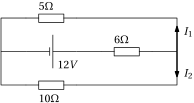
\includegraphics{t13-circuit} \end{center}

\begin{align*}
5I_1 - 10I_2 &=0\\
6(I_1+I_2)+5I_2 &=12
\end{align*}
Determine the values of \(I_1\) and \(I_2\) using a matrix method.

\begin{enumerate}
\def\labelenumi{\arabic{enumi}.}
\setcounter{enumi}{3}
\item
  Solve the equations using a determinant method:
  \begin{align*}
  \frac{3}{x}-\frac{2}{y} &= 0.5\\
  \frac{5}{x}-\frac{3}{y} &= 2.57
  \end{align*}
\item
  A vector system to determine the shortest distance between two moving bodies is analysed and produces the following equations:
  \begin{align*}
  11s_1 - 10s_2 &= 30\\
  21s_2 - 20s_1 &= -40
  \end{align*}
  Using Cramer's rule solve for \(s_1\) and \(s_2\).
\item
  The law connecting friction, \(F\), and load, \(L\), for an experiment to establish the friction force between two surfaces is of the form \(F = aL + b\), where both \(a\) and \(b\) are constants.
  When \(F = 6\), \(L = 7.5\) and when \(F = 2.7\), \(L = 2\), determine the values of \(a\) and \(b\) using a matrix method.
\end{enumerate}

\emph{Solutions:}
\textbf{1.} (i) \(x=55/19\), \(y=29/19\);
(ii) \(x=3\), \(y=-2\);
(iii) \(x=230/31\), \(y=160/31\);
\textbf{2.} \(x=-4\), \(y=-4\);
\textbf{3.} \(I_1=24/23\), \(I_2=12/23\);
\textbf{4.} \(x=0.27\), \(y=0.19\);
\textbf{5.} \(s_1=230/31\), \(s_2=160/31\);
\textbf{6.} \(a=0.6\), \(b=1.5\)

\hypertarget{circular-measure}{%
\chapter{Circular measure}\label{circular-measure}}

\hypertarget{radians-and-degrees}{%
\section{Radians and degrees}\label{radians-and-degrees}}

Angles are normally measured in \textbf{degrees}, e.g.~a right angle has \(90^\circ\). In mathematics and engineering it is more natural and convenient to measure angles in \textbf{radians}: the length of an arc of a unit circle is equal to the measurement, \emph{in radians}, of the angle that it subtends.

\begin{figure}

{\centering 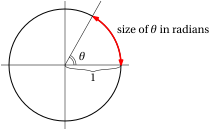
\includegraphics{t14-circle} 

}

\caption{Unit circle and radians}\label{fig:unnamed-chunk-161}
\end{figure}

\begin{longtable}[]{@{}
  >{\raggedright\arraybackslash}p{(\columnwidth - 14\tabcolsep) * \real{0.08}}
  >{\centering\arraybackslash}p{(\columnwidth - 14\tabcolsep) * \real{0.09}}
  >{\centering\arraybackslash}p{(\columnwidth - 14\tabcolsep) * \real{0.08}}
  >{\centering\arraybackslash}p{(\columnwidth - 14\tabcolsep) * \real{0.17}}
  >{\centering\arraybackslash}p{(\columnwidth - 14\tabcolsep) * \real{0.17}}
  >{\centering\arraybackslash}p{(\columnwidth - 14\tabcolsep) * \real{0.17}}
  >{\centering\arraybackslash}p{(\columnwidth - 14\tabcolsep) * \real{0.17}}
  >{\centering\arraybackslash}p{(\columnwidth - 14\tabcolsep) * \real{0.07}}@{}}
\toprule
\endhead
degrees & \(360\) & \(180\) & \(90\) & \(60\) & \(45\) & \(30\) & \(0\) \\ \addlinespace
radians & \(2\pi\) & \(\pi\) & \(\frac{\pi}{2}\) & \(\frac{\pi}{3}\) & \(\frac{\pi}{4}\) & \(\frac{\pi}{6}\) & \(0\) \\ \addlinespace
\bottomrule
\end{longtable}

\hypertarget{converting-degrees-to-radians}{%
\subsection{Converting degrees to radians}\label{converting-degrees-to-radians}}

\[\theta^\circ = \left(\dfrac{2\pi}{360}\cdot\theta\right)\,\mathrm{rad}\]

\begin{example}
\protect\hypertarget{exm:unnamed-chunk-162}{}{\label{exm:unnamed-chunk-162} }Find the value of \(23^\circ\) in radians.
\end{example}
\begin{solution}
\iffalse{} {Solution. } \fi{}\(23^\circ = \left(\dfrac{2\pi}{360}\cdot 23\right)\,\mathrm{rad} \approx 0.4\,\mathrm{rad}\).
\end{solution}

\hypertarget{converting-radians-to-degrees}{%
\subsection{Converting radians to degrees}\label{converting-radians-to-degrees}}

\[\theta\,\mathrm{rad}=\left(\dfrac{360}{2\pi}\cdot\theta\right)^\circ\]

\begin{example}
\protect\hypertarget{exm:unnamed-chunk-164}{}{\label{exm:unnamed-chunk-164} }Find the value of \(1.5\,\mathrm{rad}\) in degrees.
\end{example}
\begin{solution}
\iffalse{} {Solution. } \fi{}\(1.5\,\mathrm{rad} = \left(\dfrac{360}{2\pi}\cdot 1.5\right)^\circ = \left(\dfrac{270}{\pi}\right)^\circ \approx 85.9^\circ\).
\end{solution}

\hypertarget{arc-and-sector}{%
\section{Arc and sector}\label{arc-and-sector}}

\hypertarget{length-of-an-arc}{%
\subsection{Length of an arc}\label{length-of-an-arc}}

The \textbf{length of an arc} of a circle is given by \(s=r\cdot\theta\), where \(r\) is the radius and \(\theta\) is the angle subtended in radians.

\begin{example}
\protect\hypertarget{exm:unnamed-chunk-166}{}{\label{exm:unnamed-chunk-166} }Determine the length \(s\) of an arc of a circle with radius \(45mm\) when the angle subtended is \(85^\circ\).
\end{example}
\begin{solution}
\iffalse{} {Solution. } \fi{}\(s=r\theta = 45\,\mathrm{mm}\cdot\left(\dfrac{2\pi}{360}\cdot 85\right) \approx 66.8\,\mathrm{mm}\).
\end{solution}

\hypertarget{area-of-a-sector}{%
\subsection{Area of a sector}\label{area-of-a-sector}}

The \textbf{area of a sector} of a disc is \(A=\left(\dfrac{\theta}{2\pi}\cdot\pi\cdot r^2\right) = \dfrac{1}{2}\cdot r^2\cdot \theta\), where \(r\) is the radius of \(\theta\) is the angle subtended in radians.

\begin{example}
\protect\hypertarget{exm:unnamed-chunk-168}{}{\label{exm:unnamed-chunk-168} }A light source spreads illumination through an angle \(130^\circ\) to a distance of \(35m\). Determine the illuminated area \(A\).
\end{example}
\begin{solution}
\iffalse{} {Solution. } \fi{}\(A=\frac12 r^2\theta = \frac12\left(35\,\mathrm{m}\right)^2\cdot\left(\dfrac{2\pi}{360}\cdot 130\right) \approx 1390\,\mathrm{m}^2\).
\end{solution}

\hypertarget{exercises-14-length-of-an-arc-and-area-of-a-sector}{%
\chapter*{Exercises 14 (Length of an arc and area of a sector)}\label{exercises-14-length-of-an-arc-and-area-of-a-sector}}
\addcontentsline{toc}{chapter}{Exercises 14 (Length of an arc and area of a sector)}

\begin{enumerate}
\def\labelenumi{\arabic{enumi}.}
\item
  Convert the following to radians:

  \begin{enumerate}
  \def\labelenumii{\roman{enumii})}
  \tightlist
  \item
    \(65^\circ\)
  \item
    \(125^\circ\)
  \item
    \(420^\circ\)
  \item
    \(1120^\circ\)
  \end{enumerate}
\item
  Convert the following to degrees

  \begin{enumerate}
  \def\labelenumii{\roman{enumii})}
  \tightlist
  \item
    \(0.94\,\mathrm{rad}\)
  \item
    \(1.72\,\mathrm{rad}\)
  \item
    \(7.325\,\mathrm{rad}\)
  \item
    \(12.5\,\mathrm{rad}\)
  \end{enumerate}
\item
  Calculate the length of an arc of a circle whose radius is \(1.15\,\mathrm{m}\) when the angle subtended at the centre is \(160^\circ\).
\item
  An arc subtends an angle of \(1.732\,\mathrm{rad}\) at the centre of a circle whilst the length of the arc is \(258\,\mathrm{mm}\). Determine the circle's diameter.
\item
  In a belt drive system, \(300\,\mathrm{mm}\) are in contact with a pulley of \(400\,\mathrm{mm}\) diameter. Determine the angle of lap in both degrees and radians.
\item
  Calculate the diameter and circumference of a circle if the area of a sector which subtends an angle of \(1.45\,\mathrm{rad}\) is \(620\,\mathrm{mm}^2\).
\item
  The exhaust ports of an engine consist of 4 ring sectors with outer radii \(50\,\mathrm{mm}\), inner radii \(22\,\mathrm{mm}\) and angle \(30^\circ\). Determine the total area of the ports.
\item
  Calculate the area of the shaded potion of the sketch given below and its percentage compared to the complete sector.
\end{enumerate}

\begin{center}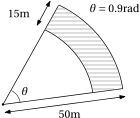
\includegraphics{t14-arc} \end{center}

\emph{Solutions:}
\textbf{1.} (i) \(1.13\); (ii) \(2.18\); (iii) \(7.33\); (iv) \(19.55\);
\textbf{2.} (i) \(53.86^\circ\); (ii) \(98.55^\circ\); (iii) \(419.69^\circ\); (iv) \(716.20^\circ\);
\textbf{3.} \(3.2\,\mathrm{m}\);
\textbf{4.} \(d=298\,\mathrm{mm}\);
\textbf{5.} \(1.5\,\mathrm{rad}\), \(85.94^\circ\);
\textbf{6.} \(58.5\,\mathrm{mm}\), \(183.7\,\mathrm{mm}\);
\textbf{7.} \(2100\,\mathrm{mm}^2\);
\textbf{8.} \(573.75\,\mathrm{m}^2\), \(51\%\)

\hypertarget{trigonometric-functions}{%
\chapter{Trigonometric functions}\label{trigonometric-functions}}

\hypertarget{from-right-triangles}{%
\section{From right triangles}\label{from-right-triangles}}

\begin{figure}

{\centering 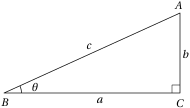
\includegraphics{t15-rtriangle1} 

}

\caption{A right triangle}\label{fig:unnamed-chunk-173}
\end{figure}

\begin{theorem}[Pythagoras's Theorem]
\protect\hypertarget{thm:unnamed-chunk-174}{}{\label{thm:unnamed-chunk-174} \iffalse (Pythagoras's Theorem) \fi{} }\(a^2+b^2=c^2\)
\end{theorem}

\emph{Proof (non-examinable):}

\begin{center}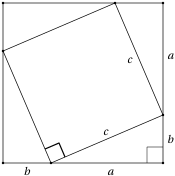
\includegraphics{t15-pythagoras} \end{center}

\begin{align*}
&&(a+b)^2 &= \text{area of the big square} = 4\left(\frac12ab\right) + c^2\\
\implies&&\quad a^2+2ab+b^2 &= 2ab+c^2\\
\implies&&\quad a^2+b^2&=c^2
\end{align*}

Returning to the figure of a right triangle above:

\begin{itemize}
\tightlist
\item
  \(AB\) is called the \textbf{hypotenuse}.
\item
  \(AC\) is the side \textbf{opposite to \(\theta\)}
\item
  \(BC\) is the side \textbf{adjacent to \(\theta\)}
\end{itemize}

\begin{center}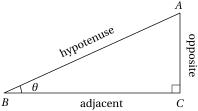
\includegraphics{t15-rtriangle2} \end{center}

The \emph{definitions} of the values of the trigonometric functions for \(\theta\) between \(0\) and \(\frac{\pi}{2}\):

\begin{itemize}
\tightlist
\item
  \(\sin\theta = \dfrac{\text{opposite}}{\text{hypotenuse}} = \dfrac{AC}{AB}\) (\textbf{sine of \(\theta\)})
\item
  \(\cos\theta = \dfrac{\text{adjacent}}{\text{hypotenuse}} = \dfrac{BC}{AB}\) (\textbf{cosine of \(\theta\)})
\item
  \(\tan\theta = \dfrac{\text{opposite}}{\text{adjacent}} = \dfrac{AC}{BC}\) (\textbf{tangent of \(\theta\)})
\item
  \(\sec\theta = \dfrac{1}{\cos\theta} = \dfrac{AB}{BC}\) (\textbf{secant of \(\theta\)})
\item
  \(\mathrm{cosec}\,\theta = \dfrac{1}{\sin\theta} = \dfrac{AB}{AC}\) (\textbf{cosecant of \(\theta\)})
\item
  \(\cot\theta = \dfrac{1}{\tan\theta} = \dfrac{BC}{AC}\) (\textbf{cotangent of \(\theta\)})
\end{itemize}

\begin{theorem}[Pythagoras's identity]
\protect\hypertarget{thm:unnamed-chunk-177}{}{\label{thm:unnamed-chunk-177} \iffalse (Pythagoras's identity) \fi{} }\(\sin^2\theta+\cos^2\theta=1\)
\end{theorem}

\emph{Proof:} \(BC^2+AC^2=AB^2\) \hfill~{(by Pythagoras's Theorem)}\\
\(\implies\) \(\left(\dfrac{BC}{AB}\right)^2+\left(\dfrac{AC}{AB}\right)^2=1\) \hfill~{(dividing by \(AB^2\))}\\
\(\implies\) \(\cos^2\theta+\sin^2\theta = 1\) \hfill~{(by the definitions above)}

\begin{example}
\protect\hypertarget{exm:unnamed-chunk-178}{}{\label{exm:unnamed-chunk-178} }Prove that \(\dfrac{1+\tan^2\theta}{1+\cot^2\theta} = \tan^2\theta\).
\end{example}
\begin{solution}
\iffalse{} {Solution. } \fi{}\begin{align*}
\mathrm{LHS} &= \frac{1+\frac{\sin^2\theta}{\cos^2\theta}}{1+\frac{\cos^2\theta}{\sin^2\theta}}\\
&= \frac{\sin^2\theta\,(\cos^2\theta+\sin^2\theta)}{\cos^2\theta\,(\sin^2\theta+\cos^2\theta)}\\
&=\frac{\sin^2\theta}{\cos^2\theta} = \tan^2\theta = \mathrm{RHS}
\end{align*}
\end{solution}

\begin{example}
\protect\hypertarget{exm:unnamed-chunk-180}{}{\label{exm:unnamed-chunk-180} }Prove that \(\sqrt{\dfrac{1-\cos\theta}{1+\cos\theta}} = \mathrm{cosec}\,\theta-\cot\theta\).
\end{example}
\begin{solution}
\iffalse{} {Solution. } \fi{}\begin{align*}
\mathrm{RHS} &= \frac{1}{\sin\theta}-\frac{\cos\theta}{\sin\theta}= \frac{1-\cos\theta}{\sin\theta}.\\
\mathrm{LHS} &= \sqrt{\frac{(1-\cos\theta)(1-\cos\theta)}{(1+\cos\theta)(1-\cos\theta)}} \\
&= \frac{\sqrt{(1-\cos\theta)^2}}{\sqrt{1-\cos^2\theta}} = \frac{1-\cos\theta}{\sqrt{\sin^2\theta}}\\
&= \frac{1-\cos\theta}{\sin\theta} = \mathrm{LHS}.
\end{align*}
\end{solution}

A table of very commonly used values:

\begin{longtable}[]{@{}
  >{\raggedright\arraybackslash}p{(\columnwidth - 10\tabcolsep) * \real{0.16}}
  >{\centering\arraybackslash}p{(\columnwidth - 10\tabcolsep) * \real{0.08}}
  >{\centering\arraybackslash}p{(\columnwidth - 10\tabcolsep) * \real{0.20}}
  >{\centering\arraybackslash}p{(\columnwidth - 10\tabcolsep) * \real{0.20}}
  >{\centering\arraybackslash}p{(\columnwidth - 10\tabcolsep) * \real{0.20}}
  >{\centering\arraybackslash}p{(\columnwidth - 10\tabcolsep) * \real{0.17}}@{}}
\toprule
\endhead
\(\theta\) & \(0\) & \(\frac{\pi}6\) & \(\frac{\pi}4\) & \(\frac{\pi}3\) & \(\frac{\pi}2\) \\ \addlinespace
\(\sin\theta\) & \(0\) & \(\frac12\) & \(\frac1{\sqrt2}\) & \(\frac{\sqrt3}2\) & \(1\) \\ \addlinespace
\(\cos\theta\) & \(1\) & \(\frac{\sqrt3}2\) & \(\frac1{\sqrt2}\) & \(\frac12\) & \(0\) \\ \addlinespace
\(\tan\theta\) & \(0\) & \(\frac1{\sqrt3}\) & \(1\) & \(\sqrt3\) & not defined \\ \addlinespace
\bottomrule
\end{longtable}

How to derive some of these?

\begin{itemize}
\tightlist
\item
  \(\theta=\frac{\pi}4\) implies \(AC=BC\), so \(\sin\theta=\cos\theta\).\\
  So from Pythagoras' Identity ``\(\sin^2\theta+\cos^2\theta=1\)'', we get\\
  \(2\sin^2\theta=1\) \(\implies\) \(\sin\theta=1/\sqrt2\).
\item
  \(\theta=\frac{\pi}{6}\): by doubling the triangle we get an equilateral one, thus\\
  \(AC=\frac12AB\). Hence \(\sin\theta=\frac{AC}{AB}=\frac12\), and also\\
  \(\cos\theta=\sqrt{1-\sin^2\theta} = \sqrt{\frac34} = \frac{\sqrt{3}}2\).
\end{itemize}

\hypertarget{as-functions}{%
\section{As functions}\label{as-functions}}

Given an angle \(\theta\), let \(P=(x,y)\) be the intersection point of the unit circle with the half-line through the origin making an angle \(\theta\) with the positive half of the \(x\)-axis.

\begin{center}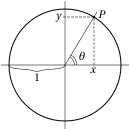
\includegraphics{t15-circle1} \end{center}

Then, by the definition of trig functions above:
\begin{align*}
x&= \cos\theta,\\
y&= \sin\theta.
\end{align*}

We can take \emph{this} as the \emph{definition} of \(\sin\) and \(\cos\) (and consequently of \(\tan\), \ldots) if \(\theta\) is arbitrary (e.g.~negative, or larger than \(\frac\pi2\)).

With this, we get \textbf{basic trigonometric identities}:
\begin{align*}
    \cos(-\theta) &=\cos\theta, & \sin(-\theta) &=-\sin\theta \\
    \cos(\theta+2\pi) &=\cos\theta & \sin(\theta+2\pi) &=\sin\theta\\
    \cos(\theta+\pi) &= -\cos\theta & \sin(\theta+\pi) &= -\sin\theta\\
    \tan(\theta+\pi) &= \tan\theta & \tan(-\theta) &= -\tan\theta
\end{align*}

\begin{figure}
\centering
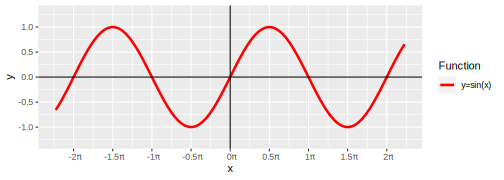
\includegraphics{fy_Alectnotes_files/figure-latex/t15-sine-1.pdf}
\caption{\label{fig:t15-sine}Graph of sine}
\end{figure}

\begin{figure}
\centering
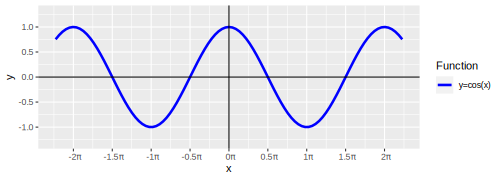
\includegraphics{fy_Alectnotes_files/figure-latex/t15-cosine-1.pdf}
\caption{\label{fig:t15-cosine}Graph of cosine}
\end{figure}

\begin{figure}
\centering
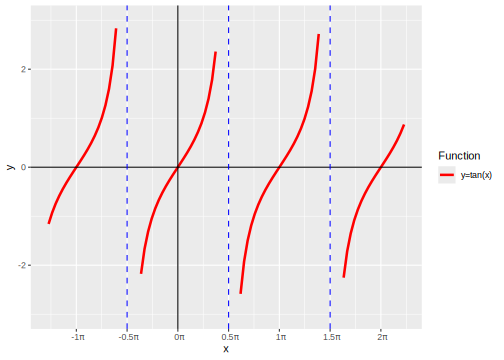
\includegraphics{fy_Alectnotes_files/figure-latex/t15-tangent-1.pdf}
\caption{\label{fig:t15-tangent}Graph of tangent}
\end{figure}

\hypertarget{inverse-trigonometric-functions}{%
\section{Inverse trigonometric functions}\label{inverse-trigonometric-functions}}

Given \(-1\leq x\leq 1\), we let \(\arcsin x\) \(= \theta\), such that \(\sin\theta = x\) and \(-\frac\pi2\leq\theta\leq \frac\pi2\).

Given \(-1\leq x\leq 1\), we let \(\arccos x\) \(= \theta\), such that \(\cos\theta = x\) and \(0\leq\theta\leq \pi\).

Given any \(x\), we let \(\arctan x\) \(= \theta\), such that \(\tan\theta=x\) and \(-\frac\pi2\leq\theta\leq\frac\pi2\).

\begin{itemize}
\tightlist
\item
  \(\arcsin\frac12=\frac{\pi}6\)
\item
  \(\arctan 1 = \frac{\pi}{4}\)
\item
  \(\arcsin -\frac12=-\frac{\pi}6\)
\item
  \(\arccos\frac12 = \frac{\pi}3\)
\item
  \(\arcsin\frac{1}{\sqrt{2}} = \frac{\pi}{4} = \arccos\frac{1}{\sqrt{2}}\)
\item
  \(\arccos -\frac12= \frac{2\pi}{3}\)
\end{itemize}

\begin{figure}
\centering
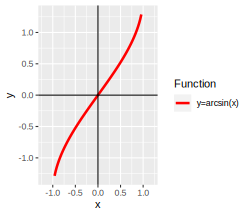
\includegraphics{fy_Alectnotes_files/figure-latex/t15-arcsin-1.pdf}
\caption{\label{fig:t15-arcsin}Graph of arcsin}
\end{figure}

\begin{figure}
\centering
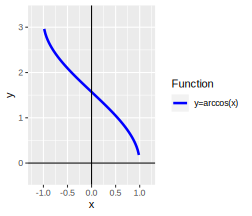
\includegraphics{fy_Alectnotes_files/figure-latex/t15-arccos-1.pdf}
\caption{\label{fig:t15-arccos}Graph of arccos}
\end{figure}

\begin{figure}
\centering
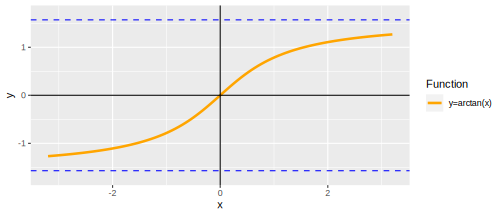
\includegraphics{fy_Alectnotes_files/figure-latex/t15-arctan-1.pdf}
\caption{\label{fig:t15-arctan}Graph of arctan}
\end{figure}

\hypertarget{exercises-15-trigonometric-functions-and-equations}{%
\chapter*{Exercises 15 (Trigonometric functions and equations)}\label{exercises-15-trigonometric-functions-and-equations}}
\addcontentsline{toc}{chapter}{Exercises 15 (Trigonometric functions and equations)}

\begin{enumerate}
\def\labelenumi{\arabic{enumi}.}
\item
  Determine all the angles between \(0^\circ\) and \(360^\circ\) whose

  \begin{enumerate}
  \def\labelenumii{\roman{enumii})}
  \tightlist
  \item
    sine is \(-0.4848\)
  \item
    cosine is \(0.8361\)
  \item
    tangent is \(-1.832\)
  \item
    secant is \(1.392\)
  \item
    cotangent is \(0.6848\)
  \end{enumerate}
\item
  Evaluate to 4 significant figures:
  \[
  \sec 286.08^\circ – 3.26 \,\mathrm{cosec}\, 146.72^\circ + 9 \cot 312.25^\circ.
  \]
\item
  Evaluate the following:

  \begin{enumerate}
  \def\labelenumii{\roman{enumii})}
  \tightlist
  \item
    \(\sin\frac{3\pi}{8}\)
  \item
    \(\cos\frac{5\pi}{9}\)
  \item
    \(\tan\frac{5\pi}{16}\)
  \item
    \(\sec\frac{7\pi}{12}\)
  \item
    \(\mathrm{cosec}\,4.72\pi\)
  \item
    \(\cot \frac{4\pi}{9}\)
  \end{enumerate}
\item
  Given that \(A=32.9^\circ\) and \(B=63.48^\circ\), determine to four significant figures:

  \begin{enumerate}
  \def\labelenumii{\roman{enumii})}
  \tightlist
  \item
    \(2\sec A\cot B\)
  \item
    \(\dfrac{\mathrm{cosec}\,A+\sec B}{1-\tan A\cos B}\)
  \item
    \(\dfrac{5\cot B}{4\sin A\,\mathrm{cosec}\, B}\)
  \end{enumerate}
\item
  Prove the following:

  \begin{enumerate}
  \def\labelenumii{\roman{enumii})}
  \tightlist
  \item
    \(\tan^2\theta\,(\mathrm{cosec}^2\theta -1)=1\)
  \item
    \(\tan\theta = \sqrt{\dfrac{1-\cos^2\theta}{\cos^2\theta}}\)
  \item
    \(\dfrac{\mathrm{cosec}\,\theta}{\sec\theta}-\dfrac{\sec\theta}{\mathrm{cosec}\,\theta} = (\cos^2\theta-\sin^2\theta)\sec\theta\,\mathrm{cosec}\,\theta\)
  \item
    \(\sin\theta-\sin^3\theta = \dfrac{\sin\theta}{\sec^2\theta}\)
  \end{enumerate}
\item
  Solve the equation \(8 \sin^2\theta + 2 \cos\theta = 5\), stating all the values of \(\theta\) between \(0^\circ\) and \(360^\circ\).
\item
  Solve the following equations for all values of \(x\) from \(0^\circ\) to \(360^\circ\):

  \begin{enumerate}
  \def\labelenumii{\alph{enumii})}
  \tightlist
  \item
    \(\sin x=0.3\)
  \item
    \(\cos x=-0.7\)
  \item
    \(\tan x=-0.75\)
  \item
    \(2\sin x=3\cos x\)
  \item
    \(4\sin x\cos x = 3\cos x\)
  \item
    \(4\cos^2 x+\cos x = 0\)
  \item
    \(2\sin^2 x-\sin x-1=0\)
  \item
    \(\sin x-2\cos^2 x+1=0\)
  \end{enumerate}
\item
  Solve the following equations for all values of \(x\) from \(-180^\circ\) to \(180^\circ\):

  \begin{enumerate}
  \def\labelenumii{\alph{enumii})}
  \tightlist
  \item
    \(\cos^2 x=0.75\)
  \item
    \(\sin 2x = 2\cos 2x\)
  \item
    \(3\sin^2 x=2\sin x\cos x\)
  \item
    \(2\cos^2 x-5\cos x+2=0\)
  \item
    \(\sin^2 x+\cos x+1=0\)
  \item
    \(\sin^2 x+5\cos^2 x =3\)
  \end{enumerate}
\end{enumerate}

\emph{Solutions:}
\textbf{1.} (i) \(209^\circ\), \(331^\circ\);
(ii) \(33.3^\circ\), \(326.7^\circ\);
(iii) \(118.6^\circ\), \(298.6^\circ\);
(iv) \(44.1^\circ\), \(315.9^\circ\);
(v) \(55.6^\circ\), \(235,6^\circ\);
\textbf{2.} \(-10.51\);
\textbf{3.} (i) \(0.92\);
(ii) \(-0.17\);
(iii) \(1.497\);
(iv) \(-3.86\)
(v) \(1.298\);
(vi) \(0.18\);
\textbf{4.} (i) \(1.189\);
(ii) \(5.738\);
(iii) \(1.027\);
\textbf{6.} \(41.9^\circ\), \(318.6^\circ\), or \(120^\circ\), \(240^\circ\);
\textbf{7.} (a) \(17.5^\circ\), \(162.5^\circ\);
(b) \(134.4^\circ\), \(225.6^\circ\);
(c) \(143.1^\circ\), \(323.1^\circ\);
(d) \(56.3^\circ\), \(236.3^\circ\);
(e) \(48.6^\circ\), \(90^\circ\), \(131.4^\circ\), \(270^\circ\);
(f) \(90^\circ\), \(104.5^\circ\), \(255.5^\circ\), \(270^\circ\);
(g) \(90^\circ\), \(210^\circ\), \(330^\circ\);
(h) \(30^\circ\), \(150^\circ\), \(270^\circ\);
\textbf{8.}
(a) \(\pm 30^\circ\), \(\pm150^\circ\);
(b) \(-148.3^\circ\), \(-58.3^\circ\), \(31.7^\circ\), \(121.7^\circ\);
(c) \(0^\circ\), \(33.7^\circ\), \(-146.3^\circ\), \(\pm180^\circ\);
(d) \(\pm 60^\circ\);
(e) \(\pm180^\circ\);
(f) \(\pm45^\circ\), \(\pm135^\circ\)

\hypertarget{rectangular-cartesian-coordinates}{%
\chapter{Rectangular (Cartesian) coordinates}\label{rectangular-cartesian-coordinates}}

\begin{figure}

{\centering 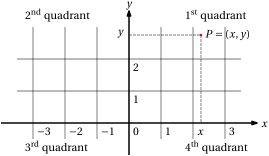
\includegraphics{t16-cart} 

}

\caption{Cartesian coordinate system}\label{fig:unnamed-chunk-185}
\end{figure}

\(x\) and \(y\) are called the \textbf{Cartesian} (or \textbf{rectangular}) coordinates of \(P\).

The whole plane is split by the coordinate axes into four regions called \textbf{quadrants}.

\begin{figure}

{\centering 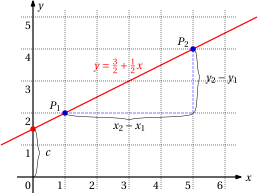
\includegraphics{t16-line} 

}

\caption{Line graph}\label{fig:unnamed-chunk-186}
\end{figure}

The graph of a function of the form \(f(x)=mx+c\) is a line; \(m\) is called the \textbf{slope}; and \(c\) is the \textbf{intercept} of the line. Note: \(c=f(0)\).

If \(P_1=(x_1,y_1)\) and \(P_2=(x_2,y_2)\) are any two distinct points on the line, then \(m=\dfrac{y_2-y_1}{x_2-x_1}\).

\hypertarget{guessing-a-law-from-an-experiment}{%
\section{Guessing a law from an experiment}\label{guessing-a-law-from-an-experiment}}

Experimental data for two (physical) variables \(x,y\) can be plotted as points
in the \((x,y)\)-plane. Sometimes they may look like they roughly lie on a line.
This would indicate a linear law between \(x\) and \(y\), i.e.~\(y=mx+c\) for some numbers \(m\) and \(c\). The constants can be measured from the plot (explained in a video).

For an example, see Table \ref{tab:t16-vttable} and Figure \ref{fig:t16-vtgraph}.

\begin{table}

\caption{\label{tab:t16-vttable}Measured data: v against t}
\centering
\begin{tabular}[t]{r|r}
\hline
t (s) & v (m/s)\\
\hline
1 & 7.7\\
\hline
2 & 10.5\\
\hline
3 & 13.3\\
\hline
4 & 15.5\\
\hline
5 & 16.3\\
\hline
6 & 20.5\\
\hline
7 & 23.0\\
\hline
\end{tabular}
\end{table}

\begin{figure}
\centering
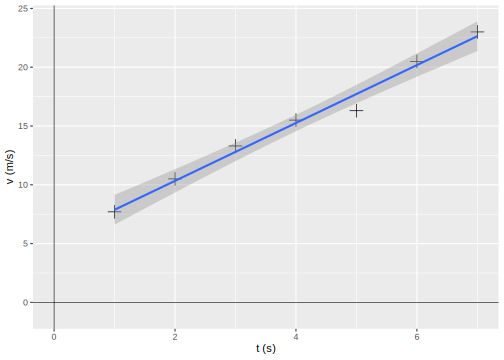
\includegraphics{fy_Alectnotes_files/figure-latex/t16-vtgraph-1.pdf}
\caption{\label{fig:t16-vtgraph}Plotted v against t}
\end{figure}

Note: sometimes the plotted data may exhibit a different ``shape''. It is useful
to learn to ``recognise'' at least quadratics, exponentials and sine/cosine.

\emph{Extra Note (non-examinable)}: Nowadays one would use statistics/linear algebra to find the ``best line'' that fits the measured data. The most commonly used method for this is called \href{https://en.wikipedia.org/wiki/Linear_regression}{linear regression} (this is what the blue line in Figure \ref{fig:t16-vtgraph} actually represents).

\hypertarget{exercises-16-plotting-in-rectangular-coordinates}{%
\chapter*{Exercises 16 (Plotting in rectangular coordinates)}\label{exercises-16-plotting-in-rectangular-coordinates}}
\addcontentsline{toc}{chapter}{Exercises 16 (Plotting in rectangular coordinates)}

\begin{enumerate}
\def\labelenumi{\arabic{enumi}.}
\tightlist
\item
  The strain \(\varepsilon\) induced in a wire when subjected to a series of stress \(\sigma\) values produced the following results:
\end{enumerate}

\begin{longtable}[]{@{}
  >{\raggedright\arraybackslash}p{(\columnwidth - 10\tabcolsep) * \real{0.41}}
  >{\raggedright\arraybackslash}p{(\columnwidth - 10\tabcolsep) * \real{0.12}}
  >{\raggedright\arraybackslash}p{(\columnwidth - 10\tabcolsep) * \real{0.12}}
  >{\raggedright\arraybackslash}p{(\columnwidth - 10\tabcolsep) * \real{0.12}}
  >{\raggedright\arraybackslash}p{(\columnwidth - 10\tabcolsep) * \real{0.12}}
  >{\raggedright\arraybackslash}p{(\columnwidth - 10\tabcolsep) * \real{0.12}}@{}}
\toprule
\endhead
\(\sigma\) (M Pa) & \(10.8\) & \(21.6\) & \(33.3\) & \(37.8\) & \(45.9\) \\ \addlinespace
\(\varepsilon\) (\(\times 10^{-5}\)) & \(12\) & \(24\) & \(37\) & \(42\) & \(51\) \\ \addlinespace
\bottomrule
\end{longtable}

Show that the stress is related to the strain by a law of the form \(\sigma=E\varepsilon\), where \(E\) is a constant.
Determine the law for the wire under test.

\begin{enumerate}
\def\labelenumi{\arabic{enumi}.}
\setcounter{enumi}{1}
\tightlist
\item
  During a test on a simple lifting machine, the following results were obtained showing the
  applied force, \(F\), for the load, \(L\), lifted:
\end{enumerate}

\begin{longtable}[]{@{}
  >{\raggedright\arraybackslash}p{(\columnwidth - 12\tabcolsep) * \real{0.17}}
  >{\raggedright\arraybackslash}p{(\columnwidth - 12\tabcolsep) * \real{0.12}}
  >{\raggedright\arraybackslash}p{(\columnwidth - 12\tabcolsep) * \real{0.14}}
  >{\raggedright\arraybackslash}p{(\columnwidth - 12\tabcolsep) * \real{0.14}}
  >{\raggedright\arraybackslash}p{(\columnwidth - 12\tabcolsep) * \real{0.14}}
  >{\raggedright\arraybackslash}p{(\columnwidth - 12\tabcolsep) * \real{0.14}}
  >{\raggedright\arraybackslash}p{(\columnwidth - 12\tabcolsep) * \real{0.14}}@{}}
\toprule
\endhead
\(F\) (N) & \(19\) & \(37\) & \(50\) & \(93\) & \(125\) & \(149\) \\ \addlinespace
\(L\) (N) & \(40\) & \(120\) & \(230\) & \(410\) & \(540\) & \(680\) \\ \addlinespace
\bottomrule
\end{longtable}

It is thought that the equation relating \(F\) and \(L\) is of the form \(F = kL + c\) where both \(k\) and \(c\) are constants. Assuming that the law holds true, find the force necessary to lift a load of \(1\,\mathrm{kN}\).

\begin{enumerate}
\def\labelenumi{\arabic{enumi}.}
\setcounter{enumi}{2}
\tightlist
\item
  The variation in pressure, \(p\), within a vessel at a temperature, \(T\), follows a law of the form \(p = aT + b\). Verify that the data below relates the data by this law and determine the law.
\end{enumerate}

\begin{longtable}[]{@{}
  >{\raggedright\arraybackslash}p{(\columnwidth - 12\tabcolsep) * \real{0.19}}
  >{\raggedright\arraybackslash}p{(\columnwidth - 12\tabcolsep) * \real{0.14}}
  >{\raggedright\arraybackslash}p{(\columnwidth - 12\tabcolsep) * \real{0.14}}
  >{\raggedright\arraybackslash}p{(\columnwidth - 12\tabcolsep) * \real{0.14}}
  >{\raggedright\arraybackslash}p{(\columnwidth - 12\tabcolsep) * \real{0.14}}
  >{\raggedright\arraybackslash}p{(\columnwidth - 12\tabcolsep) * \real{0.14}}
  >{\raggedright\arraybackslash}p{(\columnwidth - 12\tabcolsep) * \real{0.14}}@{}}
\toprule
\endhead
\(p\) (kPa) & \(248\) & \(253\) & \(257\) & \(262\) & \(266\) & \(270\) \\ \addlinespace
\(T\) (K) & \(273\) & \(278\) & \(283\) & \(288\) & \(293\) & \(298\) \\ \addlinespace
\bottomrule
\end{longtable}

\begin{enumerate}
\def\labelenumi{\arabic{enumi}.}
\setcounter{enumi}{3}
\item
  Determine graphically the solution to the simultaneous equations:
  \begin{align*}
  2.5x + 0.45 - 3y &= 0\\
  1.6x + 0.8y - 0.8 &= 0
  \end{align*}
\item
  Plot graphs of:

  \begin{enumerate}
  \def\labelenumii{\roman{enumii})}
  \tightlist
  \item
    \(y = 2x^2\)
  \item
    \(y = 2x^2 - 4\)
  \item
    \(y = 2x^2 - 2x + 0.5\)
  \item
    \(y = 2x^2 + x - 6\)
  \end{enumerate}
\item
  Plot the graph of \(y = 4x^3 - 4x^2 - 15x + 18\) for values of \(x\) from \(-3\) to \(+3\) and using the graph, determine the roots of the polynomial.
\item
  On the same axes and to the same scale plot the equations \(y = 1.5e^{-1.18x}\) and \(y = 1.1(1 - e^{-2.3x})\). Determine the solution to the equations from your graph.
\end{enumerate}

\hypertarget{parametric-representation}{%
\chapter{Parametric representation}\label{parametric-representation}}

Sometimes the variables \(x\) and \(y\) are themselves functions of another variable, called \textbf{parameter}, say \(x=x(t)\) and \(y=y(t)\). We may be able to express \(y\) in terms of \(x\) by eliminating \(t\).

\begin{example}
\protect\hypertarget{exm:unnamed-chunk-189}{}{\label{exm:unnamed-chunk-189} }\(x=a\cos\theta\), ~ \(y=a\sin\theta\), where \(a\) is a positive constant and \(\theta\) is the parameter.
\end{example}

We aim to eliminate \(\theta\) and express \(y\) in terms of \(x\).\\
We square both equations and add them: \(x^2=a^2\sin^2\theta\), ~ \(y^2=a^2\cos^2\theta\)\\
\(\implies\) \(x^2+y^2=a^2(\cos^2\theta+\sin^2\theta) = a^2\)\\
\(\implies\) \(y=\pm\sqrt{a^2-x^2}\) ~ (thus in this case, there are two ``branches'' of the function: one with the ``+'' and one with the ``-''; see Figure \ref{fig:t17-circle}).

\begin{figure}
\centering
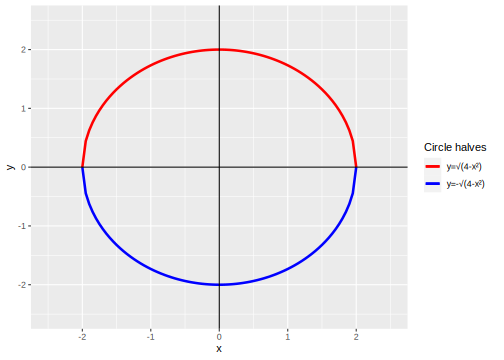
\includegraphics{fy_Alectnotes_files/figure-latex/t17-circle-1.pdf}
\caption{\label{fig:t17-circle}Graph of ±√(4-x²)}
\end{figure}

\begin{example}
\protect\hypertarget{exm:unnamed-chunk-190}{}{\label{exm:unnamed-chunk-190} }A curve is given by \(x=t^2\) and \(y=2t\). Find its Cartesian equation.
\end{example}
\begin{solution}
\iffalse{} {Solution. } \fi{}
1. \(y=2t\) \(\implies\) \(t^2=\frac{y^2}{4}\)\\
2. \(x=t^2\)

Putting 1. and 2. together, we get \(x=\frac{y^2}{4}\) \(\iff\) \(y=\pm2\sqrt{x}\). See Figure \ref{fig:t17-sqrt}.
\end{solution}

\begin{figure}
\centering
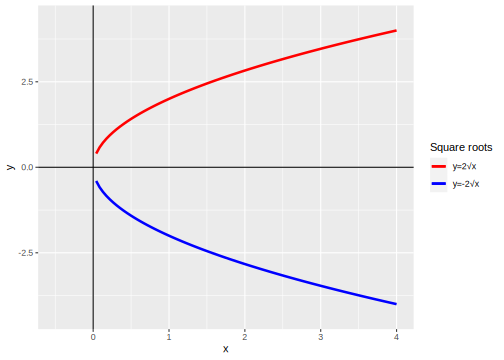
\includegraphics{fy_Alectnotes_files/figure-latex/t17-sqrt-1.pdf}
\caption{\label{fig:t17-sqrt}Graph of ±2√x}
\end{figure}

\hypertarget{exercises-17-parametric-representation}{%
\chapter*{Exercises 17 (Parametric representation)}\label{exercises-17-parametric-representation}}
\addcontentsline{toc}{chapter}{Exercises 17 (Parametric representation)}

\begin{enumerate}
\def\labelenumi{\arabic{enumi}.}
\item
  Plot the functions given below in parametric form for the range \(0\) to \(2\pi\,\mathrm{rad}\):

  \begin{enumerate}
  \def\labelenumii{\roman{enumii})}
  \tightlist
  \item
    \(x = 10\cos\theta\), \(y = 10\sin\theta\)
  \item
    \(x = 10\cos\theta\), \(y = 5\sin\theta\)
  \end{enumerate}
\item
  Let \(t\) vary from \(-4\) to \(+4\) for \(x = 1 - t\), \(y = t\) and plot the function. Also eliminate the variable \(t\) to express \(x\) in terms of \(y\).
\item
  For the equations below, stated in parametric form, eliminate the parameter \(t\) to obtain the Cartesian form. Assume \(a\) and \(c\) are constants.

  \begin{enumerate}
  \def\labelenumii{\roman{enumii})}
  \tightlist
  \item
    \(x = at^2\), ~ ~ \(y = 2at\)
  \item
    \(x = ct\), ~ ~ \(y=\frac{c}{t}\)
  \item
    \(x = 2t + 1\), ~ ~ \(y = 2t(t - 1)\)
  \end{enumerate}
\end{enumerate}

\emph{Solutions:}
\textbf{2.} \(y=1-x\);
\textbf{3.} (i) \(y^2=4ax^2\);
(ii) \(y=\frac{c^2}{x}\);
(iii) \(y=\frac{x^2-4x+3}{2}\)

\hypertarget{polar-coordinates}{%
\chapter{Polar coordinates}\label{polar-coordinates}}

\begin{figure}

{\centering 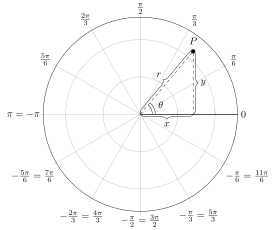
\includegraphics{t18-polar-pics-1} 

}

\caption{Polar coordinates chart}\label{fig:t18-polar-chart}
\end{figure}

Given a point \(P\) in the plane as in Figure \ref{fig:t18-polar-chart}:

\begin{itemize}
\tightlist
\item
  \(r\) and \(\theta\) are called the \textbf{polar coordinates} of \(P\), also written as \(r\angle\theta\) or \([r\angle\theta]\).
\item
  The \textbf{principal angle convention} is that \(-\pi<\theta\leq\pi\). This makes \(\theta\) uniquely determined by \(P\).
\item
  The convention \(0\leq\theta<2\pi\) is often used as well.
\end{itemize}

\hypertarget{converting-polar-to-cartesian-coordinates}{%
\section{Converting polar to Cartesian coordinates}\label{converting-polar-to-cartesian-coordinates}}

\begin{figure}

{\centering 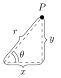
\includegraphics{t18-polar-pics-2} 

}

\caption{Conversion triangle}\label{fig:t18-triangle}
\end{figure}

Given a point \(P=[r\angle\theta]\) as in Figure \ref{fig:t18-triangle}, its Cartesian coordinates are given by the following formulas:

\[\boxed{x=r\cos\theta, \quad y=r\sin\theta}\]

\begin{example}
\protect\hypertarget{exm:unnamed-chunk-194}{}{\label{exm:unnamed-chunk-194} }\([2\sqrt2\angle \frac\pi4] = (2\sqrt{2}\cdot\frac{1}{\sqrt2},2\sqrt{2}\cdot\frac{1}{\sqrt2})=(2,2)\).
\end{example}

\begin{example}
\protect\hypertarget{exm:unnamed-chunk-195}{}{\label{exm:unnamed-chunk-195} }\([6.8\angle 55^\circ] = (6.8\cos 55^\circ,6.8\sin 55^\circ) \approx(3.9,5.6)\).
\end{example}

\hypertarget{converting-cartesian-to-polar-coordinates}{%
\section{Converting Cartesian to polar coordinates}\label{converting-cartesian-to-polar-coordinates}}

Given a point \(P=(x,y)\) as in Figure \ref{fig:t18-triangle}, its polar coordinates are given by the following formulas:

\[\boxed{r=\sqrt{x^2+y^2}}\]

\[\boxed{\theta=\begin{cases}
        \arctan(\frac{y}{x}) & \text{if }x>0\\
        \arctan(\frac{y}{x})+\pi &\text{if }x<0\text{ and }y\geq0\\
        \arctan(\frac{y}{x})-\pi &\text{if }x<0\text{ and }y<0\\
        \frac{\pi}2&\text{if }x=0\text{ and }y>0\\
        -\frac{\pi}2&\text{if }x=0\text{ and }y<0\\
        \text{undefined} &\text{if }x=0\text{ and }y=0
\end{cases}}\]

\emph{Note:} The value of ``\(\arctan(\dots)\)'' is a quantity that describes \emph{size of an angle}. The formula above assumes that it is in \emph{radians} (hence the appearance of \(\pi\)). Some care is required when using a calculator which can be set to work in \emph{degrees} instead, in which case the above formulas need to be adjusted by replacing every \(\pi\) by \(180^\circ\).

\begin{example}
\protect\hypertarget{exm:t18-cart-to-polar}{}{\label{exm:t18-cart-to-polar} }\begin{align*}
(-67.4,20.31) &= \left[\sqrt{(-67.4)^2+(20.31)^2}\angle \left(\arctan\left(\frac{20.31}{-67.4}\right)+\pi\right)\cdot\frac{180^\circ}{\pi}\right]\\
&\approx\left[70.39\angle 163.23^\circ\right]
\end{align*}
\end{example}

\begin{example}
\protect\hypertarget{exm:unnamed-chunk-196}{}{\label{exm:unnamed-chunk-196} }Six holes in the plane are given, each in polar coordinates relative to the preceding one: see Table \ref{tab:t18-holes-table}. Sketch the system and determine the coordinates of hole 6 relative to hole 1 in rectangular and polar coordinates.
\end{example}

\begin{longtable}[]{@{}
  >{\raggedright\arraybackslash}p{(\columnwidth - 2\tabcolsep) * \real{0.12}}
  >{\raggedleft\arraybackslash}p{(\columnwidth - 2\tabcolsep) * \real{0.38}}@{}}
\caption{\label{tab:t18-holes-table} Relative polar coordinates of holes in the plane}\tabularnewline
\toprule
Hole & Relative polar coordinates \\ \addlinespace
\midrule
\endfirsthead
\toprule
Hole & Relative polar coordinates \\ \addlinespace
\midrule
\endhead
Hole 1 & \(90\angle 120^\circ\) \\ \addlinespace
Hole 2 & \(40\angle 90^\circ\) \\ \addlinespace
Hole 3 & \(55\angle 60^\circ\) \\ \addlinespace
Hole 4 & \(25\angle 45^\circ\) \\ \addlinespace
Hole 5 & \(20\angle-30^\circ\) \\ \addlinespace
Hole 6 & \(150\angle -150^\circ\) \\ \addlinespace
\bottomrule
\end{longtable}

\begin{solution}
\iffalse{} {Solution. } \fi{}For a sketch, see Figure \ref{fig:t18-holes-sketch}.

Use the above formulas to convert \emph{relative polar} coordinates to \emph{relative Cartesian} coordinates: see Table \ref{tab:t18-holes-table-filled}. Cartesian coordinates of hole 6 relative to hole 1 are the sum of the rectangular coordinates of holes 2 to 6. Executing this we arrive at: \((-67.4,20.31)\).

We convert back to polar coordinates (see Example \ref{exm:t18-cart-to-polar}) and obtain the polar coordinates of hole 6 relative to hole 1 as: \(70.39\angle 163.23^\circ\).
\end{solution}

\begin{figure}

{\centering 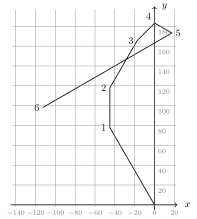
\includegraphics{t18-polar-pics-3} 

}

\caption{A diagram for the example of holes in the plane}\label{fig:t18-holes-sketch}
\end{figure}

\begin{longtable}[]{@{}
  >{\raggedright\arraybackslash}p{(\columnwidth - 4\tabcolsep) * \real{0.12}}
  >{\raggedleft\arraybackslash}p{(\columnwidth - 4\tabcolsep) * \real{0.38}}
  >{\raggedleft\arraybackslash}p{(\columnwidth - 4\tabcolsep) * \real{0.38}}@{}}
\caption{\label{tab:t18-holes-table-filled} Relative polar and Cartesian coordinates of holes}\tabularnewline
\toprule
Hole & Relative polar coords & Relative Cartesian coords \\ \addlinespace
\midrule
\endfirsthead
\toprule
Hole & Relative polar coords & Relative Cartesian coords \\ \addlinespace
\midrule
\endhead
Hole 1 & \(90\angle 120^\circ\) & \((-45,77.94)\) \\ \addlinespace
Hole 2 & \(40\angle 90^\circ\) & \((0,40)\) \\ \addlinespace
Hole 3 & \(55\angle 60^\circ\) & \((27.5,47.63)\) \\ \addlinespace
Hole 4 & \(25\angle 45^\circ\) & \((17.68,17.68)\) \\ \addlinespace
Hole 5 & \(20\angle-30^\circ\) & \((17.32,-10)\) \\ \addlinespace
Hole 6 & \(150\angle -150^\circ\) & \((-129.9,-75)\) \\ \addlinespace
\bottomrule
\end{longtable}

\hypertarget{curves-in-polar-coordinates}{%
\section{Curves in polar coordinates}\label{curves-in-polar-coordinates}}

\begin{center}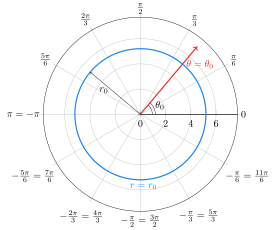
\includegraphics{t18-polar-pics-4} \end{center}

\begin{center}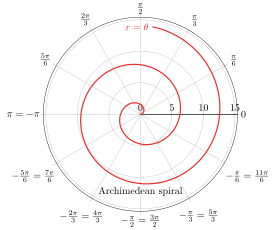
\includegraphics{t18-polar-pics-5} \end{center}

\begin{center}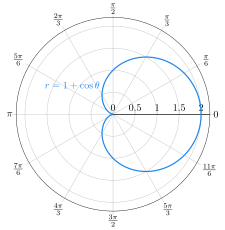
\includegraphics{t18-polar-pics-6} \end{center}

\begin{center}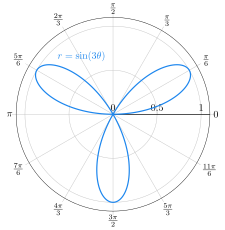
\includegraphics{t18-polar-pics-7} \end{center}

\begin{center}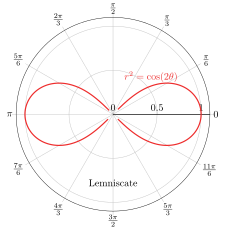
\includegraphics{t18-polar-pics-8} \end{center}

\hypertarget{exercises-18-polar-coordinates}{%
\chapter*{Exercises 18 (Polar coordinates)}\label{exercises-18-polar-coordinates}}
\addcontentsline{toc}{chapter}{Exercises 18 (Polar coordinates)}

\begin{enumerate}
\def\labelenumi{\arabic{enumi}.}
\item
  Express in polar form:

  \begin{enumerate}
  \def\labelenumii{\roman{enumii})}
  \tightlist
  \item
    \((5, 2)\)
  \item
    \((3, 7)\)
  \item
    \((-5, 2)\)
  \item
    \((-8, -9)\)
  \item
    \((17, -12)\)
  \end{enumerate}
\item
  Express in rectangular form:

  \begin{enumerate}
  \def\labelenumii{\roman{enumii})}
  \tightlist
  \item
    \(5 \angle 65^\circ\)
  \item
    \(3.8 \angle 124^\circ\)
  \item
    \(7.2 \angle -56^\circ\)
  \item
    \(15 \angle -138^\circ\)
  \end{enumerate}
\item
  Six holes are marked out in polar coordinates as:
\end{enumerate}

\begin{longtable}[]{@{}
  >{\raggedright\arraybackslash}p{(\columnwidth - 2\tabcolsep) * \real{0.12}}
  >{\raggedright\arraybackslash}p{(\columnwidth - 2\tabcolsep) * \real{0.39}}@{}}
\toprule
\endhead
Hole 1 & \(65 \angle 65^\circ\) \\ \addlinespace
Hole 2 & \(55 \angle 95^\circ\) \\ \addlinespace
Hole 3 & \(45 \angle -20^\circ\) \\ \addlinespace
Hole 4 & \(80 \angle 55^\circ\) \\ \addlinespace
Hole 5 & \(160 \angle -170^\circ\) \\ \addlinespace
Hole 6 & \(95 \angle -80^\circ\) \\ \addlinespace
\bottomrule
\end{longtable}

Sketch the system and determine the position of Hole 1 relative to Hole 6 in rectangular coordinates. The coordinates for each hole are given relative to the previous hole.

\begin{enumerate}
\def\labelenumi{\arabic{enumi}.}
\setcounter{enumi}{3}
\item
  For values of \(\theta\) in the range \(0\) to \(2\pi\), plot at intervals of \(\pi/6\) radians the functions:

  \begin{enumerate}
  \def\labelenumii{\roman{enumii})}
  \tightlist
  \item
    \(r = 2 \sin \theta\)
  \item
    \(r = 2 \cos^2\theta\)
  \item
    \(r = a(1 + 2 \cos \theta)\)
  \item
    \(r = a \cos \theta\)
  \item
    \(r = a \sin^2\theta\)
  \item
    \(r = a \sin 2\theta\)
  \item
    \(r = a \sin 3\theta\)
  \item
    \(r = a \cos 2\theta\)
  \item
    \(r = a \cos 3\theta\)
  \end{enumerate}
\end{enumerate}

Assume \(a\) is a constant.

\emph{Solutions:}
\textbf{1.} (i) \(5.38\angle21.8^\circ\);
(ii) \(7.61\angle66.8^\circ\);
(iii) \(5.38\angle158.2^\circ\);
(iv) \(12.04\angle-131.6^\circ\);
(v) \(20.8\angle -35.23^\circ\);
\textbf{2.}
(i) \((2.1,4.3)\);
(ii) \((-2.1,3.15)\);
(iii) \((4.03,-5.97)\);
(iv) \((-11.1,-10.0)\);
\textbf{3.} \((57.7,16.4)\);
\textbf{4.}

\begin{center}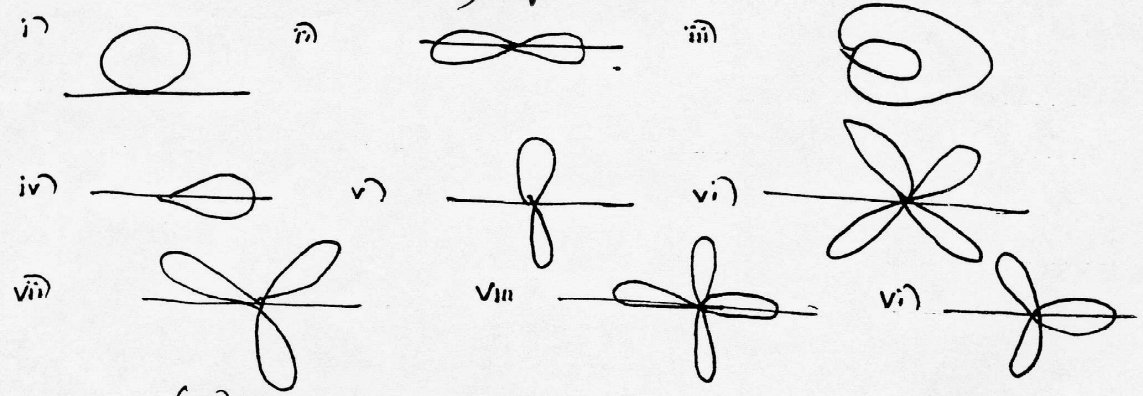
\includegraphics{t17-curves} \end{center}

\hypertarget{sine-and-cosine-rules}{%
\chapter{Sine and cosine rules}\label{sine-and-cosine-rules}}

\begin{figure}

{\centering 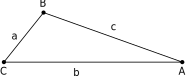
\includegraphics{fy_Alectnotes_files/figure-latex/t19-basictriangle-1} 

}

\caption{Triangle ABC}\label{fig:t19-basictriangle}
\end{figure}

\begin{theorem}
\protect\hypertarget{thm:unnamed-chunk-206}{}{\label{thm:unnamed-chunk-206} }Given an arbitrary triangle (marked as on Figure \ref{fig:t19-basictriangle}), we have:

\begin{enumerate}
\def\labelenumi{\arabic{enumi}.}
\item
  \textbf{Sine Rule}: \(\boxed{\dfrac{a}{\sin A} = \dfrac{b}{\sin B} = \dfrac{c}{\sin C}}\) = diameter of the circumscribed circle.
\item
  \textbf{Cosine Rule}: \(\boxed{a^2+b^2 = c^2 + 2ab\cos C}\)\\
  and variants:\\
  \(b^2+c^2 = a^2 + 2bc\cos A\)\\
  \(a^2+c^2 = b^2 + 2ac\cos B\)
\item
  \(\boxed{\mathrm{Area} = \frac12 bh = \frac12ab\sin C = \sqrt{s(s-a)(s-b)(s-c)}}\) ~ ~ where \(h\) is the \emph{height} of the triangle (see Figure \ref{fig:t19-markedtriangle}) and \(s=\dfrac{a+b+c}{2}\).\\
  (The formula with \(s\) is called \emph{Heron's formula}.)
\end{enumerate}
\end{theorem}

\emph{Proofs (non-examinable):} Start by further marking the triangle as in Figure \ref{fig:t19-markedtriangle}.

\begin{enumerate}
\def\labelenumi{\arabic{enumi}.}
\tightlist
\item
  (Sine rule) By definition of sine in the triangles \(CHB\) and \(HAB\), we have \(a\sin C=h=c\sin A\).\\
  \(\implies\) \(\dfrac{a}{\sin A}=\dfrac{c}{\sin C}\).\\
  The other equalities can be derived similarly.
\end{enumerate}

\begin{figure}

{\centering \includegraphics{fy_Alectnotes_files/figure-latex/t19-markedtriangle-1} 

}

\caption{Triangle ABC with markings}\label{fig:t19-markedtriangle}
\end{figure}

\begin{enumerate}
\def\labelenumi{\arabic{enumi}.}
\setcounter{enumi}{1}
\item
  (Cosine rule) We begin by using Pythagoras' Theorem for the triangles \(CHB\) and \(HAB\):
  \begin{align*}
  a^2-x^2 &= h^2 = c^2-(b-x)^2\\
  a^2-x^2 &=c^2-b^2+2bc - x^2\\
  a^2+b^2 &= c^2+2bx
  \end{align*}
  From the definition of cosine for the triangle \(CHB\), we have \(x=a\cos C\), which leads to
  \[
  a^2+b^2=c^2-2ab\cos C.
  \]
\item
  (Area of the triangle)
\end{enumerate}

The area of the triangle \(ABC\) is the sum of the areas of the two right triangles \(CHB\) and \(HAB\), each of which is a half of the area of a rectangle. Thus
\[
\mathrm{Area} = \frac12xh + \frac12(b-x)h = \frac12bh.
\]
Using the definition of sine for the triangle \(CHB\), we get \(h=a\sin C\), hence we get further
\[
\mathrm{Area} = \frac12ab\sin C.
\]
Deriving Heron's formula is a little more algebraically involved. Recall from above that
\begin{align*}
a^2+b^2&=c^2+2bx\\
\implies\quad\quad\quad x&=\frac{a^2+b^2-c^2}{2b}
\end{align*}
Starting now with the Pythagoras's Theorem for triangle \(CHB\), we obtain
\begin{align*}
h^2 &= a^2-x^2 = a^2-\left(\frac{a^2+b^2-c^2}{2b}\right)^2\\
&= \frac{4a^2b^2 - (a^2+b^2-c^2)^2}{4b^2}\\
&= \frac{(2ab + a^2+b^2-c^2)(2ab-a^2-b^2+c^2)}{4b^2} &&\text{NB: }X^2-Y^2=(X+Y)(X-Y)\\
&= \frac{\left((a+b)^2-c^2\right)\cdot\left(c^2 - (a+b)^2\right)}{4b^2}\\
&= \frac{(a+b+c)(a+b-c)(c+a-b)(c-a+b)}{4b^2} &&\text{NB: same trick as above}\\
&= \frac{2s\cdot 2(s-c)\cdot 2(s-b) \cdot 2(s-a)}{4b^2}
= 4\cdot\frac{s(s-a)(s-b)(s-c)}{b^2}.
\end{align*}
Consequently,
\begin{align*}
\mathrm{Area} &= \frac12bh\\
&= \frac12 b \sqrt{4\frac{s(s-a)(s-b)(s-c)}{b^2}}\\
&= \sqrt{s(s-a)(s-b)(s-c)}.
\end{align*}

\begin{center}\rule{0.5\linewidth}{0.5pt}\end{center}

To find all the sides and angles of a triangle, you may want to use the following approach:

\begin{longtable}[]{@{}
  >{\raggedright\arraybackslash}p{(\columnwidth - 2\tabcolsep) * \real{0.60}}
  >{\raggedright\arraybackslash}p{(\columnwidth - 2\tabcolsep) * \real{0.19}}@{}}
\toprule
given: & use: \\ \addlinespace
\midrule
\endhead
one side and two angles & sine rule \\ \addlinespace
two sides and an angle (not between them) & sine rule \\ \addlinespace
two sides and the angle between them & cosine rule \\ \addlinespace
three sides & cosine rule \\ \addlinespace
\bottomrule
\end{longtable}

\begin{example}
\protect\hypertarget{exm:unnamed-chunk-207}{}{\label{exm:unnamed-chunk-207} }Calculate the angles of a triangle with sides of length \(a=80\,\mathrm{mm}\), \(b=70\,\mathrm{mm}\), \(c=50\,\mathrm{mm}\).
\end{example}

\begin{solution}
\iffalse{} {Solution. } \fi{}Using the cosine rule, we calculate
\begin{align*}
\cos A &= \frac{b^2+c^2-a^2}{2bc}\\
&= \frac{70^2+50^2-80^2}{2\cdot70\cdot50} =\frac{1}{7} \approx 0.1429
\end{align*}
\(\implies\) \(\angle A = \arccos 0.1429 \approx 81.78^\circ\).

Using the sine rule, we calculate
\begin{align*}
\sin B &= b\cdot \frac{\sin A}{a}\\
&= 70 \cdot \frac{\sin 81.78^\circ}{80} \approx 0.866
\end{align*}
\(\implies\) \(\angle B=\arcsin 0.866 \approx 60^\circ\)\\
\(\implies\) \(\angle C = 180^\circ-\angle A-\angle B= 38.22^\circ\).
\end{solution}

\begin{example}
\protect\hypertarget{exm:unnamed-chunk-209}{}{\label{exm:unnamed-chunk-209} }Determine the area of a triangle with \(a=6\,\mathrm{m}\), \(b=5\,\mathrm{m}\), \(c=9\,\mathrm{m}\).
\end{example}

\begin{solution}
\iffalse{} {Solution. } \fi{}We use Heron's formula:
\begin{align*}
s&=\frac{a+b+c+}{2}=\frac{6\,\mathrm{m} + 5\,\mathrm{m}+ 9\,\mathrm{m}}{2}=10\,\mathrm{m}\\
\implies\quad\quad\quad\mathrm{Area} &= \sqrt{s(s-a)(s-b)(s-c)}\\
&= \sqrt{10\,\mathrm{m}\cdot 4\,\mathrm{m}\cdot 5\,\mathrm{m}\cdot 1\,\mathrm{m}} \\
&= \sqrt{200\,\mathrm{m^4}} \approx 14.14\,\mathrm{m^2}.
\end{align*}
\end{solution}

\begin{example}
\protect\hypertarget{exm:unnamed-chunk-211}{}{\label{exm:unnamed-chunk-211} }Determine all sides, angles and area of a triangle with \(b=10\,\mathrm{m}\), \(c=5\,\mathrm{m}\) and \(\angle A=120^\circ\).
\end{example}
\begin{solution}
\iffalse{} {Solution. } \fi{}First, we use cosine rule to determine \(a\):
\begin{align*}
a^2 &= b^2+c^2-2bc\cos A\\
&= 100\,\mathrm{m^2} + 25 \,\mathrm{m^2} - 2\cdot 10\,\mathrm{m}\cdot 5\,\mathrm{m}\cdot \cos 120^\circ\\
&= 125\,\mathrm{m^2} + 50 \,\mathrm{m^2} = 175 \,\mathrm{m^2}\\
\implies\quad\quad\quad a &= \sqrt{175\,\mathrm{m^2}} =5\sqrt{7}\,\mathrm{m} \approx 13.23\,\mathrm{m}.
\end{align*}

Second, we use sine rule to calculate \(\angle B\):
\begin{align*}
\sin B &= b\cdot\frac{\sin A}{a}\\
&= 10\,\mathrm{m}\cdot \frac{\sin 120^\circ}{5\sqrt{7}\,\mathrm{m}} = \frac{10\cdot \frac{\sqrt{3}}{2}}{5\sqrt{7}} =\frac{\sqrt{3}}{\sqrt{7}}\approx 0.6547\\
\implies\quad\quad\quad \angle B &= \arcsin 0.6547 \approx 40.9^\circ.
\end{align*}

Third, we calculate
\[
\angle C = 180^\circ - \angle A-\angle B = 180^\circ- 120^\circ - 40.9^\circ = 19.1^\circ.
\]

Finally, we can use (for example) Heron's formula to obtain the area:
\begin{align*}
s &= \frac{a+b+c}{2} = \frac{10+5+5\sqrt{7}}{2}\,\mathrm{m} \approx 14.12\,\mathrm{m}\\
\implies\quad\quad\quad \mathrm{Area} &= 
\sqrt{s(s-a)(s-b)(s-c)}\\
&=\sqrt{14.12\cdot 0.89\cdot 4.12\cdot 9.12} \,\mathrm{m^2} \approx 21.73\,\mathrm{m^2}.
\end{align*}
\end{solution}

\hypertarget{exercises-19-sine-and-cosine-rules}{%
\chapter*{Exercises 19 (Sine and cosine rules)}\label{exercises-19-sine-and-cosine-rules}}
\addcontentsline{toc}{chapter}{Exercises 19 (Sine and cosine rules)}

\begin{enumerate}
\def\labelenumi{\arabic{enumi}.}
\tightlist
\item
  For the simple crank mechanism \(ABC\), given that \(AB = 60\,\mathrm{mm}\) and \(BC = 170\,\mathrm{mm}\), calculate the distance \(AC\) when the angle at \(B\) is \(140^\circ\).
\end{enumerate}

\begin{center}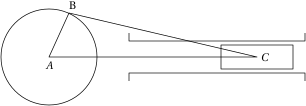
\includegraphics{t19-crank} \end{center}

\begin{enumerate}
\def\labelenumi{\arabic{enumi}.}
\setcounter{enumi}{1}
\item
  A scalene triangle \(ABC\) has the lengths of the sides set out as \(AB = 65\,\mathrm{mm}\), \(AC = 95\,\mathrm{mm}\) and \(BC = 80\,\mathrm{mm}\). Determine to the nearest degree the value of each angle.
\item
  Three holes are marked on a pitch circle with chordal distances as shown below. Determine
  the values for the angles \(BAC\) and \(ABC\) and the pitch circle diameter.
\end{enumerate}

\begin{center}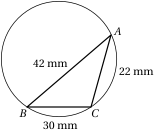
\includegraphics{t19-circle} \end{center}

\begin{enumerate}
\def\labelenumi{\arabic{enumi}.}
\setcounter{enumi}{3}
\tightlist
\item
  A mass \(m\) is suspended by two wires from a horizontal beam. If \(PK=3.3\,\mathrm{m}\), \(KQ=4.7\,\mathrm{m}\) and \(PQ=5\,\mathrm{m}\), determine the angle \(PQK\) and the vertical distance of \(K\) below the beam.
\end{enumerate}

\begin{center}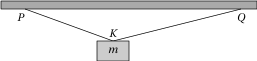
\includegraphics{t19-beam} \end{center}

\begin{enumerate}
\def\labelenumi{\arabic{enumi}.}
\setcounter{enumi}{4}
\tightlist
\item
  Calculate the coordinates \(x\) and \(y\) of the centre of the hole relative to the two axes shown.
\end{enumerate}

\begin{center}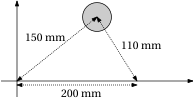
\includegraphics{t19-hole} \end{center}

\emph{Solutions:}
\textbf{1.} \(219.4\,\mathrm{mm}\);
\textbf{2.} \(56.3^\circ\), \(42.6^\circ\), \(81.1^\circ\);
\textbf{3.} \(43.16^\circ\), \(30.1^\circ\), \(43.87\,\mathrm{mm}\);
\textbf{4.} \(39.6^\circ\), \(3.00\,\mathrm{m}\);
\textbf{5.} \((126,81.4)\)

\hypertarget{compound-and-multiple-angles}{%
\chapter{Compound and multiple angles}\label{compound-and-multiple-angles}}

\begin{theorem}[Compound angle formulas for sine and cosine]
\protect\hypertarget{thm:t20-compsin}{}{\label{thm:t20-compsin} \iffalse (Compound angle formulas for sine and cosine) \fi{} }\[
\boxed{
\begin{array}{rcl}
\sin(\alpha+\beta) &=& \sin\alpha\cos\beta + \cos\alpha\sin\beta\\
\cos(\alpha+\beta) &=& \cos\alpha\cos\beta - \sin\alpha\sin\beta
\end{array}
}\]
\end{theorem}

\emph{Proof of Theorem \ref{thm:t20-compsin} (non-examinable):}

First, we will arrange points in the plane to arrive at Figure \ref{fig:t20-diagram}.

\begin{itemize}
\tightlist
\item
  Define \(E\) by \(|AE|=1\).
\item
  Define \(C\) so that \(\angle ACE=90^\circ\).
\item
  Define \(B\) so that \(\angle ABC=90^\circ\).
\item
  Form rectangle \(ABDF\), so that \(E\) lies on \(DF\).
\end{itemize}

\begin{figure}

{\centering 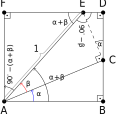
\includegraphics{fy_Alectnotes_files/figure-latex/t20-diagram-1} 

}

\caption{Diagram for the proof of compound angle formulas}\label{fig:t20-diagram}
\end{figure}

Then:
\begin{align}
|CE| &= \sin\beta, & |AC| &= \cos\beta \tag{\(\triangle ACE\)}\\
|EF| &= \cos(\alpha+\beta), & |AF| &=\sin(\alpha+\beta) \tag{\(\triangle AEF\)}
\end{align}
This implies that
\begin{align}
|AB| &= \cos\alpha\cos\beta, & |BC| &= \sin\alpha\cos\beta \tag{\(\triangle ABC\)}\\
|CD| &= \cos\alpha\sin\beta, & |DE| &= \sin\alpha\sin\beta \tag{\(\triangle CDE\)}
\end{align}
Hence
\begin{align*}
\sin(\alpha+\beta) &= |AF| = |BD| = |BC|+|CD| = \sin\alpha\cos\beta+\cos\alpha\sin\beta\\
\cos(\alpha+\beta) &= |EF| = |DF| - |DE| = \cos\alpha\cos\beta - \sin\alpha\sin\beta
\end{align*}
This finishes the proof.

\begin{corollary}[Compound angle formula for tangent]
\protect\hypertarget{cor:t20-comptan}{}{\label{cor:t20-comptan} \iffalse (Compound angle formula for tangent) \fi{} }\[\boxed{
  \tan(\alpha+\beta) = \frac{\tan\alpha+\tan\beta}{1-\tan\alpha\tan\beta}
}\]
\end{corollary}

\emph{Proof of Corollary \ref{cor:t20-comptan} using Theorem \ref{thm:t20-compsin}:}
\begin{align*}
\tan(\alpha+\beta) &= \frac{\sin(\alpha+\beta)}{\cos(\alpha+\beta)}\\
 &= \frac{\sin\alpha\cos\beta + \cos\alpha\sin\beta}{\cos\alpha\cos\beta - \sin\alpha\sin\beta} &&\text{(by Theorem)}\\
 &= \frac{\frac{\sin\alpha}{\cos\alpha} + \frac{\sin\beta}{\cos\beta}}{1-\frac{\sin\alpha\sin\beta}{\cos\alpha\cos\beta}}
 = \frac{\tan\alpha+\tan\beta}{1-\tan\alpha\tan\beta}.
\end{align*}
(For the penultimate step, we divide both top and bottom by \(\cos\alpha\cos\beta\).)

\begin{corollary}[Double angle formulas]
\protect\hypertarget{cor:t20-double}{}{\label{cor:t20-double} \iffalse (Double angle formulas) \fi{} }\[\boxed{
\begin{array}{rcl}
\sin(2\alpha) &=& 2\sin\alpha\cos\alpha\\
\cos(2\alpha) &=& 2\cos^2\alpha - 1 = 1-2\sin^2\alpha\\
\tan(2\alpha) &=& \dfrac{2\tan\alpha}{1-\tan^2\alpha}
\end{array}
}\]
\end{corollary}

\emph{Proof of double angle cosine formula (Corollary \ref{cor:t20-double}):}
\begin{align*}
\cos(2\alpha) &= \cos\alpha\cos\alpha - \sin\alpha\sin\alpha   &&\text{(by Theorem)}\\
&= \cos^2\alpha-\sin^2\alpha\\
&= 2\cos^2\alpha - 1 = 1-2\sin^2\alpha.
\end{align*}
(For the last step, we use Pythagoras's formula: \(\sin^2\alpha+\cos^2\alpha=1\).)

\begin{example}
\protect\hypertarget{exm:unnamed-chunk-219}{}{\label{exm:unnamed-chunk-219} }Express \(\cos(3\alpha)\) in terms of \(\cos\alpha\).
\end{example}

\begin{solution}
\iffalse{} {Solution. } \fi{}\begin{align*}
\cos(3\alpha) &=
\cos(2\alpha+\alpha) \\
&= \cos(2\alpha)\cos\alpha - \sin(2\alpha)\sin\alpha\\
&= (2\cos^2\alpha-1)\cos\alpha - (2\sin\alpha\cos\alpha)\sin\alpha\\
&= 2\cos^3\alpha - \cos\alpha - 2(1-\cos^2\alpha)\cos\alpha\\
&= 4\cos^3\alpha - 3\cos\alpha.
\end{align*}
\end{solution}

\begin{example}
\protect\hypertarget{exm:unnamed-chunk-221}{}{\label{exm:unnamed-chunk-221} }Express \(\tan(3\alpha)\) in terms of \(\tan\alpha\).
\end{example}

\begin{solution}
\iffalse{} {Solution. } \fi{}\begin{align*}
\tan(3\alpha) &=
  \tan(2\alpha+\alpha)\\
&=\frac{\tan(2\alpha)+\tan\alpha}{1-\tan(2\alpha)\tan\alpha}\\
&=\frac{\frac{2\tan\alpha}{1-\tan^2\alpha}+\tan\alpha}{1-\frac{2\tan\alpha}{1-\tan^2\alpha}\cdot\tan\alpha}\\
&=\frac{2\tan\alpha+\tan\alpha(1-\tan^2\alpha)}{1-\tan^2\alpha - 2\tan\alpha\cdot\tan\alpha}\\
&=\frac{3\tan\alpha-\tan^3\alpha}{1-3\tan^2\alpha}.
\end{align*}
\end{solution}

\begin{corollary}[Changing sums of (co)sines into products]
\protect\hypertarget{cor:t20-prods}{}{\label{cor:t20-prods} \iffalse (Changing sums of (co)sines into products) \fi{} }\[\boxed{
\begin{array}{rcl}
\sin\alpha + \sin\beta &=& 2\sin\tfrac{\alpha+\beta}2\cos\tfrac{\alpha-\beta}2\\
\sin\alpha - \sin\beta &=& 2\cos\tfrac{\alpha+\beta}2\sin\tfrac{\alpha-\beta}2\\
\cos\alpha + \cos\beta &=& 2\cos\tfrac{\alpha+\beta}2\cos\tfrac{\alpha-\beta}2\\
\cos\alpha - \cos\beta &=& - 2\sin\tfrac{\alpha+\beta}2\sin\tfrac{\alpha-\beta}2\\
\end{array}
}\]
\end{corollary}

\emph{Proof of Corollary \ref{cor:t20-prods} (non-examinable):}

Note that \(\frac{\alpha+\beta}2+\frac{\alpha-\beta}2 = \alpha\) and
\(\frac{\alpha+\beta}2-\frac{\alpha+\beta}2=\beta\). Then
\begin{align*}
\sin\alpha+\sin\beta &= \sin\left(\tfrac{\alpha+\beta}2+\tfrac{\alpha-\beta}2\right) +
  \sin\left(\tfrac{\alpha+\beta}2-\tfrac{\alpha-\beta}2\right)\notag\\
 &= \sin\tfrac{\alpha+\beta}2\cos\tfrac{\alpha-\beta}2 + \cos\tfrac{\alpha+\beta}2\sin\tfrac{\alpha-\beta}2 \notag\\
 &\phantom{=}\,\,
  + \sin\tfrac{\alpha+\beta}2\cos\left(-\tfrac{\alpha-\beta}2\right) + \cos\tfrac{\alpha+\beta}2\sin\left(-\tfrac{\alpha-\beta}2\right) \notag\\
 &= 2\sin\tfrac{\alpha+\beta}2\cos\tfrac{\alpha-\beta}2,
\end{align*}
since \(\cos(-x)=\cos(x)\) and \(\sin(-x)=-\sin(x)\). The rest are similar.

\begin{example}
\protect\hypertarget{exm:unnamed-chunk-223}{}{\label{exm:unnamed-chunk-223} }Prove that \(\dfrac{\sin(7\theta)+\sin(5\theta)}{\cos(7\theta) - \cos(5\theta)} = -\cot\theta.\)
\end{example}

\begin{solution}
\iffalse{} {Solution. } \fi{}\begin{align*}
\mathrm{LHS} &= \frac{2\sin\frac{7\theta+5\theta}{2}\cos\frac{7\theta-5\theta}{2}}{-2\sin\frac{7\theta+5\theta}{2}\sin\frac{7\theta-5\theta}{2}}\\
&= \frac{\sin6\theta\cos\theta}{-\sin6\theta\sin\theta} = \mathrm{RHS}.
\end{align*}
\end{solution}

\begin{example}
\protect\hypertarget{exm:unnamed-chunk-225}{}{\label{exm:unnamed-chunk-225} }Express \(\sin50^\circ + \sin30^\circ\) as a product of (co)sines.
\end{example}

\begin{solution}
\iffalse{} {Solution. } \fi{}\(\sin50^\circ+\sin30^\circ = 2\sin\dfrac{50^\circ+30^\circ}{2}\cos\dfrac{50^\circ-30^\circ}{2} = 2\sin 40^\circ\cos 10^\circ\).
\end{solution}

\begin{example}
\protect\hypertarget{exm:unnamed-chunk-227}{}{\label{exm:unnamed-chunk-227} }Without a calculator, evaluate \(16\cdot\sin75^\circ\cdot \cos15^\circ\).
\end{example}

\begin{solution}
\iffalse{} {Solution. } \fi{}First, we want to find \(\alpha\) and \(\beta\) so that
\[
75^\circ=\frac{\alpha+\beta}{2}, \quad\quad\quad
15^\circ=\frac{\alpha-\beta}{2}.
\]
Solving the equations, we get \(\alpha=90^\circ\) and \(\beta=60^\circ\). Hence
\begin{align*}
16\sin 75^\circ\cos15^\circ &= 16\sin\frac{90^\circ+60^\circ}{2}\cos\frac{90^\circ-60^\circ}{2}\\
&= 8(\sin90^\circ+\sin60^\circ)\\
&= 8\left(1+\frac{\sqrt3}{2}\right) = 8 + 4\sqrt{3}.
\end{align*}
\end{solution}

\begin{example}
\protect\hypertarget{exm:unnamed-chunk-229}{}{\label{exm:unnamed-chunk-229} }Prove that \(\dfrac{\sin2\alpha}{1+\cos2\alpha}=\tan\alpha\).
\end{example}

\begin{solution}
\iffalse{} {Solution. } \fi{}\begin{align*}
\mathrm{LHS} &=
\frac{2\sin\alpha\cos\alpha}{1+2\cos^2\alpha -1}\\
&= \frac{2\sin\alpha\cos\alpha}{2\cos^2\alpha} = \frac{\sin\alpha}{\cos\alpha} = \mathrm{RHS}.
\end{align*}
\end{solution}

\hypertarget{exercises-20-compound-and-multiple-angles}{%
\chapter*{Exercises 20 (Compound and multiple angles)}\label{exercises-20-compound-and-multiple-angles}}
\addcontentsline{toc}{chapter}{Exercises 20 (Compound and multiple angles)}

\begin{enumerate}
\def\labelenumi{\arabic{enumi}.}
\item
  Without using a calculator find:

  \begin{enumerate}
  \def\labelenumii{\roman{enumii})}
  \tightlist
  \item
    \(\sin 15^\circ\)
  \item
    \(\cos 15^\circ\)
  \item
    \(\tan 15^\circ\)
  \item
    \(\sin 105^\circ\)
  \item
    \(\cos 105^\circ\)
  \end{enumerate}
\item
  If \(\cos A = 0.6\) and \(\cos B = 0.8\), determine without using a calculator the values of \(\sin (A + B)\) and \(\cos(A + B)\).
\item
  Given that \(\cos A = 0.2\) and \(\cos B = 0.5\), find without using a calculator, the values of
  \(\sin (A + B)\) and \(\cos (A - B)\).
\item
  Prove that \(\sin(\theta+45^\circ)=\frac{1}{\sqrt{2}}(\sin\theta+\cos\theta)\).
\item
  If \(\tan(A+B)=0.75\) and \(\tan A=2\), determine \(B\).
\item
  Show that \(\sin (\theta + 90^\circ) + \cos (\theta - 180^\circ) = 0\).
\item
  Determine the acute angle \(\theta\), which satisfies the equation \(3 \cos (\theta - 14^\circ) = 4 \sin \theta\).
\item
  Prove that:

  \begin{enumerate}
  \def\labelenumii{\roman{enumii})}
  \tightlist
  \item
    \(\dfrac{\cos2\theta}{\cos\theta+\sin\theta}=\cos\theta-\sin\theta\)
  \item
    \(\dfrac{1-\cos2\theta}{1+\cos2\theta}=\tan^2\theta\)
  \end{enumerate}
\item
  Show that \(\sin 3A = 3\sin A - 4\sin^3 A\).
\item
  Express as a sum or difference:

  \begin{enumerate}
  \def\labelenumii{\roman{enumii})}
  \tightlist
  \item
    \(2\cos 5\theta \cos 3\theta\)
  \item
    \(\sin 25^\circ \cos 65^\circ\)
  \item
    \(\cos 3x \cos x\)
  \item
    \(\sin 5x \cos x\)
  \item
    \(2\sin (x + y) \sin (x - y)\)
  \end{enumerate}
\item
  Show that \(\sin(\theta+45^\circ)\sin(45^\circ-\theta) = -\frac{1}{2}\cos2\theta\).
\item
  Prove that \(\dfrac{\sin A+\sin 3A + \sin 5A}{\cos A+\cos 3A+\cos 5A}=\tan3A\).
\item
  Prove that \(\dfrac{\sin A-\sin 5A +\sin 9A -\sin13A}{\cos A-\cos 5A-\cos 9A+\cos 13 A}=\cot 4A\).
\item
  (* difficult) Show that in any triangle \(\tan\frac{B-C}{2}=\frac{b-c}{b+c}\cot\frac{A}{2}\).
\end{enumerate}

\emph{Solutions:}
\textbf{1.} (i) \(\frac{\sqrt{3}-1}{2\sqrt{2}}\); (ii) \(\frac{\sqrt{3}+1}{2\sqrt{2}}\); (iii) \(\frac{\sqrt{3}-1}{\sqrt{3}+1}\); (iv) \(\frac{\sqrt{3}+1}{2\sqrt{2}}\); (v) \(\frac{1-\sqrt{3}}{2\sqrt{2}}\);
\textbf{2.} \(\sin(A+B)=1\), \(\cos(A+B)=0\);
\textbf{3.} \(\sin(A+B)=0.6631\), \(\cos(A-B)=0.7485\);
\textbf{5.} \(B=-26.6^\circ\);
\textbf{7.} \(\theta= 41.6^\circ\);
\textbf{10.} (i) \(\cos8\theta+\cos2\theta\);
(ii) \(\frac12(1-\sin40^\circ)\);
(iii) \(\frac12(\cos 4x+\cos2x)\);
(iv) \(\frac12(\sin6x+\sin4x)\);
(v) \(\cos2y-\cos2x\)

\end{document}
